% The document class supplies options to control rendering of some standard
% features in the result.  The goal is for uniform style, so some attention 
% to detail is *vital* with all fields.  Each field (i.e., text inside the
% curly braces below, so the MEng text inside {MEng} for instance) should 
% take into account the following:
%
% - author name       should be formatted as "FirstName LastName"
%   (not "Initial LastName" for example),
% - supervisor name   should be formatted as "Title FirstName LastName"
%   (where Title is "Dr." or "Prof." for example),
% - degree programme  should be "BSc", "MEng", "MSci", "MSc" or "PhD",
% - dissertation title should be correctly capitalised (plus you can have
%   an optional sub-title if appropriate, or leave this field blank),
% - dissertation type should be formatted as one of the following:
%   * for the MEng degree programme either "enterprise" or "research" to
%     reflect the stream,
%   * for the MSc  degree programme "$X/Y/Z$" for a project deemed to be
%     X%, Y% and Z% of type I, II and III.
% - year              should be formatted as a 4-digit year of submission
%   (so 2014 rather than the accademic year, say 2013/14 say).

\documentclass[ % the name of the author
                    author={Tim Nguyen},
                % the name of the supervisor
                supervisor={Dr. David Bernhard},
                % the degree programme
                    degree={MEng},
                % the dissertation    title (which cannot be blank)
                     title={Implementing CSS conic gradients in the Firefox rendering engine},
                % the dissertation subtitle (which can    be blank)
                  subtitle={},
                % the dissertation     type
                      type={enterprise},
                % the year of submission
                      year={2020} ]{dissertation}

\begin{document}


% =============================================================================

% This macro creates the standard UoB title page by using information drawn
% from the document class (meaning it is vital you select the correct degree 
% title and so on).

\maketitle

% After the title page (which is a special case in that it is not numbered)
% comes the front matter or preliminaries; this macro signals the start of
% such content, meaning the pages are numbered with Roman numerals.

\frontmatter

% This macro creates the standard UoB declaration; on the printed hard-copy,
% this must be physically signed by the author in the space indicated.

\makedecl




% LaTeX automatically generates a table of contents, plus associated lists 
% of figures, tables and algorithms.  The former is a compulsory part of the
% dissertation, but if you do not require the latter they can be suppressed
% by simply commenting out the associated macro.


\tableofcontents
\listoffigures
% \listoftables
% \listofalgorithms
% \lstlistoflistings

% The following sections are part of the front matter, but are not generated
% automatically by LaTeX; the use of \chapter* means they are not numbered.

% -----------------------------------------------------------------------------

\chapter*{Executive Summary}

% {\bf A compulsory section, of at most $1$ page} 

With the web being increasingly used for modern applications, having powerful web technologies is more and more important nowadays. This project aims to implement CSS conic gradients into Firefox, the second most used desktop web browser, open source and developed by Mozilla.

According to `Can I use' \cite{caniuse-conic-gradients}, conic gradients were implemented and enabled by default in:

\begin{itemize}
    \item Google Chrome 69 (released in September 2018)
    \item Microsoft Edge since it switched to Chromium (in January 2020)
    \item Safari 12.1 (released in March 2019)
\end{itemize}

With the complexity of browser rendering engines and of the Firefox development process in mind, making an implementation of a web standard that is interoperable with other web browsers is not an easy task, since it requires extensive programming, testing and collaboration.

Despite those challenges, conic gradients have been implemented for most platforms (macOS, Linux, some Windows devices and Android) behind a feature flag in Firefox 75, released on April 8th. Once the feature flag is enabled, web developers will be able to use conic gradients more widely without a polyfill and Mozilla will be able to catch up to the competition.


% This section should pr\'{e}cis the project context, aims and objectives,
% and main contributions (e.g., deliverables) and achievements; the same 
% section may be called an abstract elsewhere.  The goal is to ensure the 
% reader is clear about what the topic is, what you have done within this 
% topic, {\em and} what your view of the outcome is.

% \noindent
% The latter aspects should (ideally) be presented as a concise, factual 
% bullet point list.  Again the points will differ for each project, but 
% an might be as follows:

% \begin{quote}
% \noindent
% \begin{itemize}
% \item I spent $120$ hours collecting material on and learning about the 
%       Java garbage-collection sub-system. 
% \item I wrote a total of $5000$ lines of source code, comprising a Linux 
%       device driver for a robot (in C) and a GUI (in Java) that is 
%       used to control it.
% \item I designed a new algorithm for computing the non-linear mapping 
%       from A-space to B-space using a genetic algorithm, see page $17$.
% \item I implemented a version of the algorithm proposed by Jones and 
%       Smith in [6], see page $12$, corrected a mistake in it, and 
%       compared the results with several alternatives.
% \end{itemize}
% \end{quote}

% -----------------------------------------------------------------------------


\chapter*{Supporting Technologies}

% {\bf A compulsory section, of at most $1$ page}

\begin{itemize}
\item I used parts of pre-existing code written for the linear and radial gradient implementations in Gecko and altered it to support parts of my implementation.
\item I used Mozilla's infrastructure for parts of the Firefox development process.
\item A Skia library method was used to support the Skia graphics backend implementation in Gecko.
\item Some test cases and examples were inspired by examples on Lea Verou polyfill's website at \url{https://leaverou.github.io/conic-gradient}.
\end{itemize}


% -----------------------------------------------------------------------------

\chapter*{Acknowledgements}

% {\bf An optional section, of at most $1$ page}

\noindent
Credits go to the following people for making this project a success:
\begin{itemize}
\item The Firefox Layout Team in particular to Jonathan Watt and Sean Voisen for finding this project
\item The Firefox Graphics Team for WebRender code reviews and answering questions related to WebRender
\item Dr. David Bernhard for supervising this project
\item Emilio Cobós Álvarez for most code reviews and answering questions related to the Firefox Style System
\item Lea Verou for being behind the original specification and for making the very helpful conic gradient polyfill
\item Lee Salzman for Skia code reviews
\item Markus Stange and Matt Woodrow for web painting code reviews
\item James Graham and Gabriel Luong for some other code reviews
\end{itemize}
% =============================================================================

% After the front matter comes a number of chapters; under each chapter,
% sections, subsections and even subsubsections are permissible.  The
% pages in this part are numbered with Arabic numerals.  Note that:
%
% - A reference point can be marked using \label{XXX}, and then later
%   referred to via \ref{XXX}; for example Chapter\ref{chap:context}.
% - The chapters are presented here in one file; this can become hard
%   to manage.  An alternative is to save the content in seprate files
%   the use \input{XXX} to import it, which acts like the #include
%   directive in C.

\mainmatter

% This chapter should describe the project context, and motivate each of
% the proposed aims and objectives.  Ideally, it is written at a fairly 
% high-level, and easily understood by a reader who is technically 
% competent but not an expert in the topic itself.

% In short, the goal is to answer three questions for the reader.  First, 
% what is the project topic, or problem being investigated?  Second, why 
% is the topic important, or rather why should the reader care about it?  
% For example, why there is a need for this project (e.g., lack of similar 
% software or deficiency in existing software), who will benefit from the 
% project and in what way (e.g., end-users, or software developers) what 
% work does the project build on and why is the selected approach either
% important and/or interesting (e.g., fills a gap in literature, applies
% results from another field to a new problem).  Finally, what are the 
% central challenges involved and why are they significant? 
 
% The chapter should conclude with a concise bullet point list that 
% summarises the aims and objectives.  For example:

% \begin{quote}
% \noindent
% The high-level objective of this project is to reduce the performance 
% gap between hardware and software implementations of modular arithmetic.  
% More specifically, the concrete aims are:

% \begin{enumerate}
% \item Research and survey literature on public-key cryptography and
%       identify the state of the art in exponentiation algorithms.
% \item Improve the state of the art algorithm so that it can be used
%       in an effective and flexible way on constrained devices.
% \item Implement a framework for describing exponentiation algorithms
%       and populate it with suitable examples from the literature on 
%       an ARM7 platform.
% \item Use the framework to perform a study of algorithm performance
%       in terms of time and space, and show the proposed improvements
%       are worthwhile.
% \end{enumerate}
% \end{quote}

% -----------------------------------------------------------------------------

\chapter{Background}
\label{chap:context}

\vspace{1cm} 

\noindent
Conic gradients, also known as angular gradients or sweep gradients, are gradients where
color stops are placed at different angles around a circle. The resulting image looks
like a cone, hence the name conic gradient. The \texttt{conic-gradient} function has been 
suggested to the CSS standards by Lea Verou \cite{blog-post-lea-verou}, currently an HCI 
researcher at the MIT Computer Science \& Artificial Intelligence Lab \cite{about-lea-verou}. 

This project is about implementing this function on the Firefox rendering engine, Gecko, currently used on Android, Linux, macOS, Windows and for printers. Firefox for iOS is not fully relevant to this project given that all iOS web browsers are restricted to use the WebKit rendering engine, although this project has uncovered a bug in WebKit's implementation, which will be described later on.

To understand the usefulness of this project, it is important to first describe the
challenges behind the conception of web technologies.


\section{Anatomy of a web page}
Web pages are documents written using markup languages like HTML.
HTML is an XML-based language, where content is described via tags:

\begin{minted}{html}
<!DOCTYPE html>
<html>
<head>
    <title>Hello world</title>
    <link rel="stylesheet" href="style.css">
</head>
<body>
    <p>This is a paragraph</p>
</body>
</html>
\end{minted}

Scripting for web pages can be done via JavaScript and associated to the HTML page via a \texttt{<script>} tag.

The Cascading Style Sheets (CSS) programming language can be used to define styling (background images, text colors, etc.) for documents written in HTML, XHTML, SVG or other markup languages typically used along with web pages.

\subsection{CSS}

A CSS file or stylesheet contains a set of CSS rules, which themselves contain a CSS selector defining which elements should be styled, and a set of CSS properties and values which defines how those elements should be styled.

For instance, the following CSS rule gives all paragraphs white text and a blue background:
\begin{minted}{css}
p {
    background-color: blue;
    color: white;
}
\end{minted}

CSS selectors have the concept of specificity which handle the case of conflicting rules: the rule which has the selector of the highest specificity will take precedence. This will not be defined in detail, since it is not highly relevant to this project.

CSS also comes with functions, like the \texttt{conic-gradient} function, which can be used as any image value:

\begin{minted}{css}
div {
    background-image: conic-gradient(red, blue);
}
\end{minted}

\noindent CSS was originally small enough that it evolved in versions:

\begin{enumerate}
    \item CSS 1, published in 1996 \cite{css-1-release}: It had support for basic alignment, color, layout and text-related properties.
    \item CSS 2, published in 1998 \cite{css-2-release}: It added support for layering via z-index, positioning, media queries, bidirectional text (for RTL languages) and shadows.
    \item CSS 2.1, with the final publication done in 2010 \cite{css-2.1-release}: It aimed to fix problems from CSS 2 by removing some features.
\end{enumerate}

CSS was then split into multiple modules, like the ``CSS Backgrounds and Borders Module'' or the ``CSS Fonts Module'' which evolve via levels for which the process will be described in the next section. The version commonly referred to as ``CSS 3'' is in reality a set of modules, but such a version does not officially exist.

\section{Web standards}

Web standards are mainly done by two bodies:
\begin{itemize}
    \item the WHATWG (Web Hypertext Application Technology Working Group), originally founded by individuals from Apple, Mozilla and Opera Software in 2004, in reaction to W3C's direction towards XHTML and lack of interest for HTML and web developer needs. Since then, individuals from Google or Microsoft have joined. \cite{whatwg-faq}
    \item the W3C (World Wide Web Consortium), the original standard organisation behind web standards founded by Tim Berners-Lee, consisting of full-time staff and member organisations. \cite{w3c-about}
\end{itemize}


After an agreement between the two bodies in 2019, the WHATWG maintains the HTML and DOM (Document Object Model) standards. Whereas the W3C maintains standards for CSS, SVG and most other web technologies. The W3C used to maintain their own version of the HTML standard before this agreement. \cite{blog-post-whatwg-w3c}


For W3C standards like CSS, the process for which a first draft becomes a recommended standard goes as follows (Quoted from \cite{w3c-consortium-process-doc}):
\begin{enumerate}
    \item Publication of the First Public Working Draft.
    \item Publication of zero or more revised Working Drafts.
    \item Publication of a Candidate Recommendation (CR).
    \item Publication of a Proposed Recommendation (PR).
    \item Publication as a W3C Recommendation (REC).
    \item Possibly, Publication as an Edited or Amended Recommendation
\end{enumerate}

When a specification reaches candidate recommendation stage, it is expected to be detailed and not require major changes. Browser vendors are recommended to implement and enable by default features from specifications only when the specification reaches at least candidate recommendation stage. In practice, it is not the case, since browser vendors often ship features from early drafts or not part of the standards. It can be done for various reasons:

\begin{itemize}
    \item The feature has consensus, but is part of a bigger specification that would take a long time to become a recommendation.
    \item It is done to find issues that arise from implementing a certain feature, in which case it is recommended to put the feature behind a feature flag.
    \item Lobbying by a browser vendor.
\end{itemize}

At the time of writing, CSS conic gradients are part of the ``CSS Image Values and Replaced Content Module Level 4'' specification \cite{css-images-4} which is a working draft. According to `Can I use' \cite{caniuse-conic-gradients}, they were implemented and enabled by default in:

\begin{itemize}
    \item Google Chrome 69 (released in September 2018)
    \item Microsoft Edge since it switched to Chromium (in January 2020)
    \item Safari 12.1 (released in March 2019)
\end{itemize}

They are currently unsupported in Internet Explorer and some other minor browsers.
Before this project, they were also completely unimplemented in Mozilla Firefox. This means that it is a web compatibility issue for websites using them.

It may be worth wondering why switching to Chromium is not being done by Mozilla when Microsoft and Opera have done it, as it would give Firefox the technology for free.

With only three major rendering engines left:
\begin{itemize}
    \item WebKit: the rendering engine used by Safari and all web browsers on iOS
    \item Blink: the rendering engine used by Chromium-based browsers (Chrome, Opera, Microsoft Edge)
    \item Gecko: Firefox's rendering engine
\end{itemize}

Diversity of rendering engines is important to prevent excessive lobbying by a single company and also helps uncover bugs in other implementations of web standards through collaboration.

\section{Web compatibility}

\subsection{Lack of support}
Imagine multiple bottle formats, each bottle having different bottle caps. If someone buys a certain bottle, they would need the appropriate bottle opener to open the bottle. 

One type of web compatibility issue is similar: if a website (the bottle) uses a technology (the bottle cap) that is only supported by one web browser (the bottle opener), the website will not be usable by every browser.

This type of issue is usually not common though, given most websites will only use technologies that are supported by most web browsers, to avoid losing out on visitors. The same is applicable to the bottle opener example, it is fairly uncommon to encounter unusual bottle caps requiring special bottle openers, as such a bottle brand would lose out on customers.

Polyfills exist to cope with this problem on websites. They act as a compatibility layer, allowing websites to use a newer technology while delivering the same content to all visitors, through older but more complex technologies.

The main problem with polyfills is that they are under the form of a JavaScript file, taking up network bandwidth when visiting production websites. JavaScript is also occasionally disabled for security reasons \cite{tor-browser-sec}. Polyfills have relatively low usage for those reasons. This justifies the usefulness of implementing the newer technology directly in all web browsers.

CSS conic gradients belong in this category of technologies with respect to the Firefox rendering engine.

\subsection{Incompatibilities}

Different forms of Badminton have evolved differently across Eurasia \cite{badminton-eurasia}. However, only one form has been standardised across the world for competitions. This allows avoiding conflicting shuttlecocks or courts. This does mean that some older courts may not be usable for competitions, leading to incompatibility.

The web had similar issues when web technologies were not well-standardised yet.
Quirks mode in HTML is an example of technology that needs to be implemented by all browser engines nowadays to support older websites. It is a set of non-standard behaviours that Microsoft Internet Explorer 5 and Netscape Navigator 4 used to have with HTML \cite{quirks-mode-mdn}. Since then, it has its own specification, which is a living standard \cite{whatwg-quirks-mode-spec}.

However, browser wars have prevented Microsoft from taking the monopoly on the browser market, when Firefox started gaining a significant usage share around 2009 and slowly killing Microsoft Internet Explorer. Although Mozilla was relatively successful democratising web standards, it was never able to win over the majority of the market \cite{statcounter-2009}, due to the arrival of WebKit and Blink: WebKit was Chrome's and Safari's engine, while Blink was Google's fork of WebKit around 2013.

With WebKit then Blink's domination, web compatibility issues continued arising, this time due to a different pattern. After the browser wars, while standards started evolving in distinct steps as defined in the previous section, these steps were relatively new, which lead to different problems, one of them being the following pattern:

\begin{enumerate}
    \item Browser A implements technology 1
    \item Browser B implements technology 2, a newer version of technology 1
    \item Website I uses technology 1
    \item Website II uses technology 2
    \item Result: Website I only works in browser A, Website II only works in browser B
\end{enumerate}

CSS linear and radial gradients are examples of such technologies. The first prefixed form was introduced in 2008 \cite{webkit-gradient}:

\begin{small}
\begin{minted}{css}
-webkit-gradient(linear, left top, left bottom, color-stop(0%, red), color-stop(100%, blue));
\end{minted}
\end{small}

The second form was introduced in 2011, with the goal of having an easier syntax to use \cite{webkit-linear-gradient}:

\begin{minted}{css}
-webkit-linear-gradient(top, red, blue);
\end{minted}

The unprefixed version was then finally introduced \cite{caniuse-gradients} (notice the slightly different first argument):

\begin{minted}{css}
linear-gradient(to bottom, red, blue);
\end{minted}

These technologies were originally implemented with prefixes to allow implementing drafts while being able to change them when they evolve into recommendations. Since the technologies were enabled by default, website production code started using the prefixed forms, making it necessary to keep supporting them for compatibility.

Conic gradients are part of a level 4 specification, which, like other new standards, takes in account web compatibility problems in the process by forcing the implementation to be done behind an internal preference until fully ready, instead of using prefixes, to prevent improper widespread use in website production code.

\section{Pre-existing gradient types}
Since a lot of the implementation is based on the pre-existing gradient types: linear and radial gradients. It is worth quickly mentioning what they are in this section.

The \texttt{-webkit-} and \texttt{-moz-} prefixed forms with a slightly different syntax are currently supported by Firefox. In fact, the \texttt{-webkit-} prefix for those two gradient types, is actually officially part of WHATWG's web compatibility standard \cite{compatibility-standard}.

\subsection{Linear gradients}

\begin{verbbox}[\small]
    background-image: linear-gradient(red, gold);
    /* equivalent to: */
    background-image: linear-gradient(red 0%, gold 100%);
    /* or: */
    background-image: linear-gradient(to bottom, red, gold);
    /* or: */
    background-image: -webkit-linear-gradient(top, red, gold);
\end{verbbox}
\begin{figure}[H]
    $\vcenter{\hbox{
\includegraphics[width=80px]{images/linear-gradient.png}}}$
    $\vcenter{\hbox{\theverbbox}}$\qquad
\end{figure}

\subsection{Radial gradients}
\begin{verbbox}[\small]
    background-image: radial-gradient(red, gold);
    /* equivalent to: */
    background-image: radial-gradient(red 0%, gold 100%);
    /* or: */
    background-image: radial-gradient(at center, red, gold);
    /* or: */
    background-image: -webkit-radial-gradient(center, red, gold);
\end{verbbox}
\begin{figure}[H]
    $\vcenter{\hbox{
\includegraphics[width=80px]{images/radial-gradient.png}}}$
    $\vcenter{\hbox{\theverbbox}}$\qquad
\end{figure}

\section{Conic gradients}

Conic gradients have been popular in the web development and web design community as some blog posts show \cite{blog-post-andrew} \cite{blog-post-alligator} \cite{blog-post-lea-verou}. The popularity can also be seen through a Twitter search for ``conic gradient'' \cite{twitter-search}, showcasing many beautiful CSS demos from the community. 

The main reason it has not been widely used is due to the lack of support in Mozilla Firefox, which many of the blog posts and tweets advocate for. Despite that last fact, the polyfill \cite{conic-gradient-polyfill} created by Lea Verou, who originally suggested the standard, has some popularity which can be seen with a non-exhaustive Github search \cite{github-search}. 

\subsection{Syntax}

The full syntax for conic gradients can be found in appendix \ref{appx:syntax}, but can be summarised as:

\begin{verbatim}
conic-gradient(
  [ from <angle> ]? [ at <position> ]?,
  <angular-color-stop-list>
)
\end{verbatim}

The function allows specifying the starting angle after the \texttt{from} keyword, where the zero angle is pointing upwards similar to a clock. The center can also be specified after the \texttt{at} keyword. Those two first parameters are optional, where the angle defaults to \texttt{0deg} and the center defaults to \texttt{50\% 50\%}.

The following figure, extracted from the specification \cite{conic-gradient-specification}, illustrates how \texttt{conic-gradient(at 25\% 30\%, white, black 60\%)} renders:

\begin{figure}[H]
    \centering
    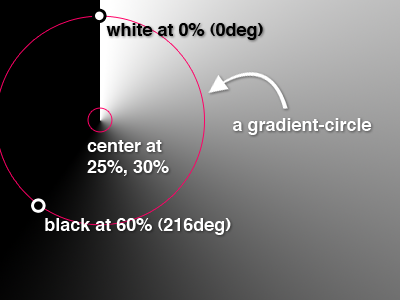
\includegraphics[width=220px]{images/conic-diagram.png}
    \caption{Example diagram of a conic-gradient}
    \label{fig:diagram-conic}
\end{figure}

After the angle and center parameters, follows the color stop list. Similarly to \texttt{linear-gradient} and \texttt{radial-gradient}, each color stop can take:

\begin{itemize}
    \item no position, where the position is interpolated implicitly
    \item one position, where the position is as specified
    \item two positions, where the stop is equivalent to specifying two stops with the same color, but at two different positions
\end{itemize}

The color stop positions are called interpolation hints or offsets.
The way stops are interpolated with each other is similar to other gradients and is defined in appendix \ref{appx:interpolation}. Unlike the other gradient types, the positions are angles or percentages, as opposed to lengths or percentages. Unless it is the first stop, color stops may omit the color, in which case it corresponds to the one from the previous stop.

Here are some more examples to illustrate how the arguments work:

\begin{verbbox}[\small]
    background-image: conic-gradient(red, gold);
    /* equivalent to: */
    background-image: conic-gradient(red 0%, gold 100%);
    /* or: */
    background-image: conic-gradient(red 0% 0%, gold 100% 100%);
    /* or: */
    background-image: conic-gradient(red 0%, 0%, gold);
\end{verbbox}
\begin{figure}[H]
    $\vcenter{\hbox{
\includegraphics[width=80px]{images/conic-example-basic.png}}}$
    $\vcenter{\hbox{\theverbbox}}$\qquad
    \caption{Simple example}
    \label{fig:conic-example-basic}
\end{figure}

\begin{verbbox}[\small]
    background-image: conic-gradient(blue .1turn, red, blue .9turn);
    /* equivalent to: */
    background-image: conic-gradient(blue 10%, red 50%, blue 90%);
    /* or: */
    background-image: conic-gradient(blue 0% 10%, red 50% 50%, blue 90% 100%);
\end{verbbox}
\begin{figure}[H]
    $\vcenter{\hbox{
\includegraphics[width=80px]{images/conic-example-cone.png}}}$
    $\vcenter{\hbox{\theverbbox}}$\qquad
    \caption{Cone example}
    \label{fig:conic-example-cone}
\end{figure}

When combined with other CSS features, it is possible to do more nice demos. The following two examples are taken from the polyfill's website \cite{conic-gradient-polyfill}.

\begin{verbbox}[\small]
    background-image: conic-gradient(red, yellow, lime, aqua, blue, magenta, red);
    border-radius: 50%;
\end{verbbox}
\begin{figure}[H]
    $\vcenter{\hbox{
\includegraphics[width=80px]{images/color-wheel.png}}}$
    $\vcenter{\hbox{\theverbbox}}$\qquad
    \caption{Color wheel example}
    \label{fig:conic-example-wheel}
\end{figure}


Since background images repeat by default, a checkerboard can be created by scaling down the background size:

\begin{verbbox}[\small]
    background-size: 20% 20%;
    background-image: conic-gradient(black 25%, white 0 50%, black 0 75%, white 0);
    /* equivalent to: */
    background-image: conic-gradient(black 25%, white 25% 50%, black 50% 75%, white 75%);
\end{verbbox}
\begin{figure}[H]
    $\vcenter{\hbox{
\includegraphics[width=80px]{images/checkerboard.png}}}$
    $\vcenter{\hbox{\theverbbox}}$\qquad
    \caption{Checkerboard example}
    \label{fig:conic-example-checkerboard}
\end{figure}

In the previous example, the first \texttt{2×2} square is the original gradient, but it is repeated across the element. This is not to be mistaken with the \texttt{repeating-conic-gradient} function described in the next section.

\subsection{Gradients with repeating stops}

A gradient with infinitely repeating stops can be specified using the \texttt{repeating-conic-gradient} function sharing the same syntax as \texttt{conic-gradient}. This function is analogous to \texttt{repeating-linear-gradient} or \texttt{repeating-radial-gradient}.

The following example creates a starburst effect:
\begin{minted}{css}
    background-image: repeating-conic-gradient(black 0 15deg, white 15deg 30deg);
\end{minted}
\begin{figure}[H]
    \centering
    
\includegraphics[width=100px]{images/repeating-conic-gradient.png}
    \caption{repeating-conic-gradient example}
    \label{fig:repeating-conic-gradient}
\end{figure}

This prevents the need for repeating the black and white stops over and over again, as it would be needed with the \texttt{conic-gradient} function:

\begin{minted}{css}
    background-image: conic-gradient(
        black 0 15deg,
        white 15deg 30deg,
        black 30deg 45deg,
        white 45deg 60deg,
        ...
        black 330deg 345deg,
        white 345deg 360deg,
    );
\end{minted}

\subsection{Other uses}

All of the examples above use the \texttt{background-image} property, since it is the most common use case, but conic gradients can be used instead of any CSS \texttt{<image>} value. This section will mention some other CSS properties that can also take image values.

\subsubsection{border-image}

The image specified by the \texttt{border-image-source} CSS property is rendered within the border specified around the element.

\begin{verbbox}[\small]
    border: 30px solid;
    border-image-source: conic-gradient(blue, red);
    background-color: lightyellow;
\end{verbbox}
\begin{figure}[H]
    $\vcenter{\hbox{
\includegraphics[width=80px]{images/border-image.png}}}$
    $\vcenter{\hbox{\theverbbox}}$\qquad
    \caption{Basic \texttt{border-image} example}
\end{figure}

It is also possible to specify how the border image should be sliced:

\begin{verbbox}[\small]
    border: 30px solid;
    border-image-source: conic-gradient(blue, red);
    border-image-slice: 1;
    background-color: lightyellow;
\end{verbbox}
\begin{figure}[H]
    $\vcenter{\hbox{
\includegraphics[width=80px]{images/border-image-2.png}}}$
    $\vcenter{\hbox{\theverbbox}}$\qquad
    \caption{\texttt{border-image-slice} example}
\end{figure}


\subsubsection{mask-image}

The mask-image property applies the image as an alpha mask on the element. Areas where the mask is opaque will be rendered, whereas areas where the mask is transparent will be masked.

\begin{verbbox}[\small]
    mask-image: conic-gradient(black, transparent);
    background-image: linear-gradient(red, gold);
\end{verbbox}
\begin{figure}[H]
    $\vcenter{\hbox{
\includegraphics[width=80px]{images/mask-image.png}}}$
    $\vcenter{\hbox{\theverbbox}}$\qquad
    \caption{\texttt{mask-image} example}
\end{figure}

% -----------------------------------------------------------------------------

\chapter{The Firefox Development process}
\label{chap:process}

\noindent
This chapter describes how to set up a development environment to build Firefox
and the Firefox development process in general. It is worth noting that due to 
the 20 year-old history of the source code, there are different workflows that 
have been developed and documented which all work today. This section will
describe the workflow that I have used for development, which should be close
to the latest recommended one.

\section{Finding issues to work on}

While some of Mozilla's projects are on Github, most older projects like
Firefox are tracked on Mozilla's own issue tracker called
Bugzilla \cite{bugzilla}.

To find simple issues to get familiar with the development process, there
are ``Good first bugs'' which can be browsed on Codetribute \cite{codetribute}.
These issues usually have mentors assigned to them and are simple changes 
with step-by-step instructions.


\section{Getting the source code}
Firefox development uses Mercurial (hg) \cite{mercurial}, a version-control system similar to Git, although Git can also be used through ports or mirrors.

The command mentioned in the documentation to clone the Firefox source code is:

\begin{verbatim}
hg clone --uncompressed https://hg.mozilla.org/mozilla-unified
\end{verbatim}

mozilla-unified is the repository combining the commit history of all other Firefox
repositories like mozilla-central, mozilla-beta or mozilla-release (which will be
described at the end of this chapter) as different branches.

The command above usually takes about 30 minutes depending on the network connection.
Once the cloning is done, the central branch should be checked out, since it contains
the latest stable changes:

\begin{verbatim}
hg up central
\end{verbatim}

\texttt{hg up} is a shortcut for \texttt{hg update}, which is equivalent to the
\texttt{git checkout} command on Git, as it lets you check out the source code at
different commits.

\section{Installing dependencies}

Once the source code is cloned, the dependencies can be installed by running the following command \cite{build-firefox}:

\begin{verbatim}
./mach bootstrap
\end{verbatim}

This will bring up an interactive wizard to install
the tools appropriate for the developer. The wizard will ask whether to use full or artifact builds at some point. Full builds are used for C++ and Rust changes, since they require the full binaries to be regenerated, while artifact builds are typically used for frontend changes where binaries can be downloaded from a server \cite{build-firefox}. For this project, full builds are necessary since the project involves changes on the rendering engine written in C++ and Rust.

\noindent On Windows, extra steps need to be done beforehand, as mentioned on the documentation \cite{windows-build-prereqs}:

\begin{quote}
    1. You need a 64-bit version of Windows 7 or later.
    
    2. Download and install Visual Studio.
    
    3. Finally download the MozillaBuild Package. Installation directory should be: \texttt{c:\textbackslash\textbackslash mozilla-build\textbackslash}
\end{quote}

\section{Building Firefox}

Once the changes have been made to the source code, in order to test the changes,
building Firefox is needed. This is done using the following command:

\begin{verbatim}
./mach build
\end{verbatim}

The first time, this command takes about one hour for full builds depending on the hardware \cite{build-firefox}, while artifact builds take about 5 minutes depending on the network connection. Once finished, the build can be ran using:

\begin{verbatim}
./mach run
\end{verbatim}

\section{Getting around the source code}

Mozilla provides a very useful search tool called Searchfox \cite{searchfox} where code is regularly indexed from different Mozilla repositories. In search results, Searchfox can distinguish between function definitions, function declarations (for C++), function calls and raw text matches. Although not showcased in the screenshot, it also displays results from test files separately for convenience and build-generated files can be also be searched through.

\begin{figure}[H]
    \centering
    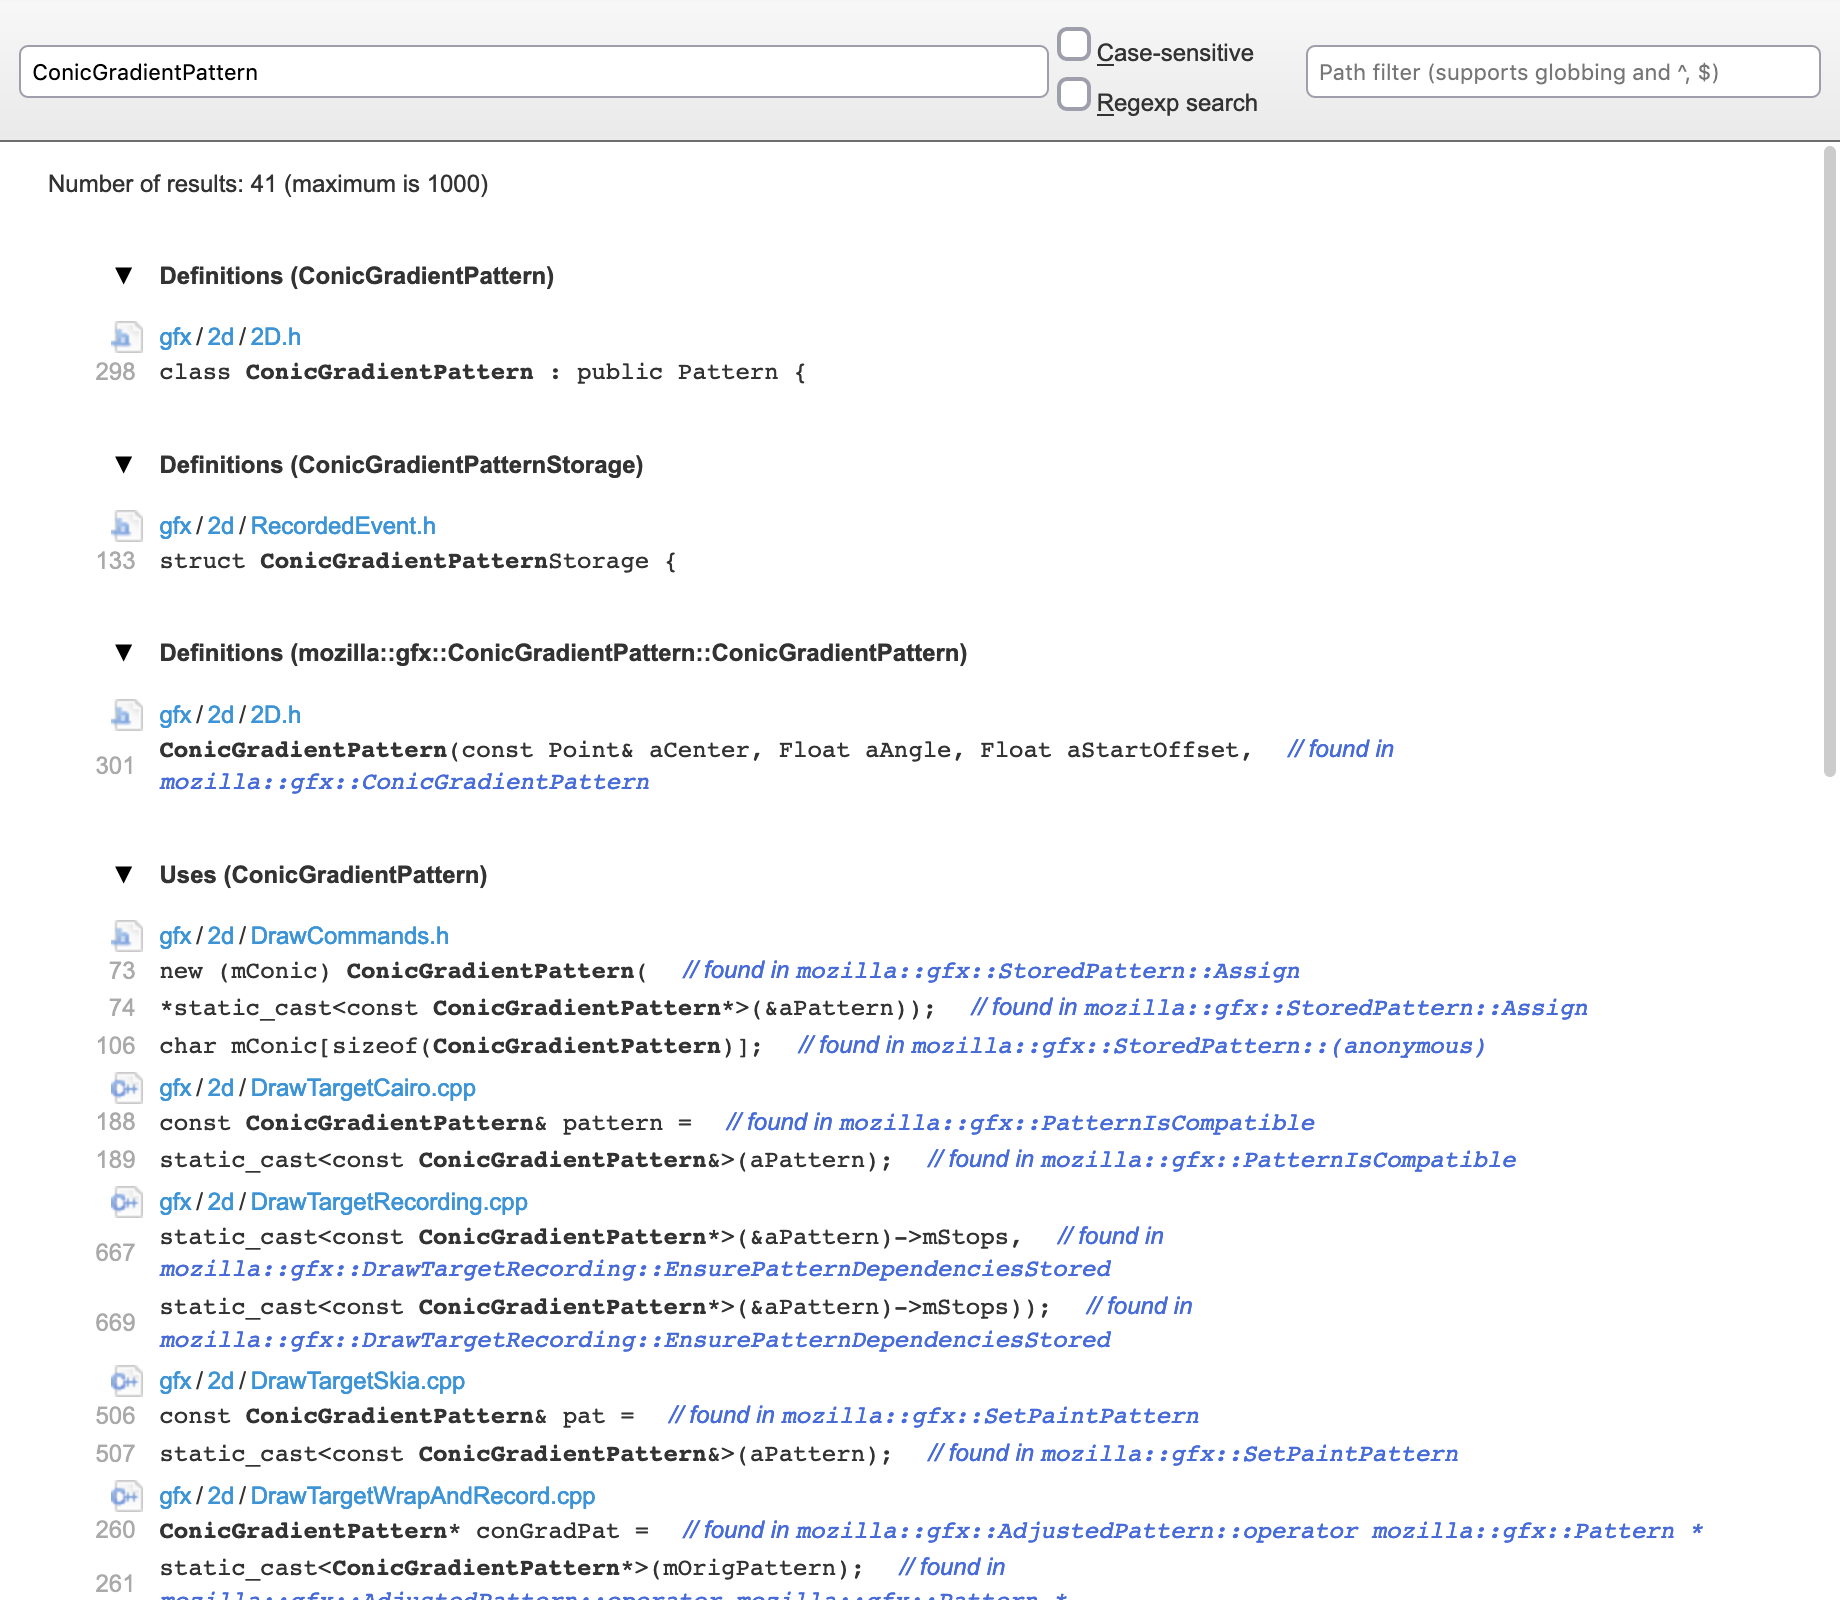
\includegraphics[width=\textwidth]{images/searchfox.png}
    \caption{Screenshot of a Searchfox search for ConicGradientPattern}
    \label{fig:searchfox}
\end{figure}

In the code view, there is an annotate (or blame) sidebar, which shows which commit added or last changed a certain line of code, and code can be browsed through different points of history if needed. 
The code view also provides different links:
\begin{itemize}
    \item a link to file a Bugzilla issue in the component relevant to the file,
    \item a link to the log showing all commits that have affected this file,
    \item a link to the raw file,
    \item links to open the file in other tools (HG Web, Code Coverage, DXR).
\end{itemize}

\begin{figure}[H]
    \centering
    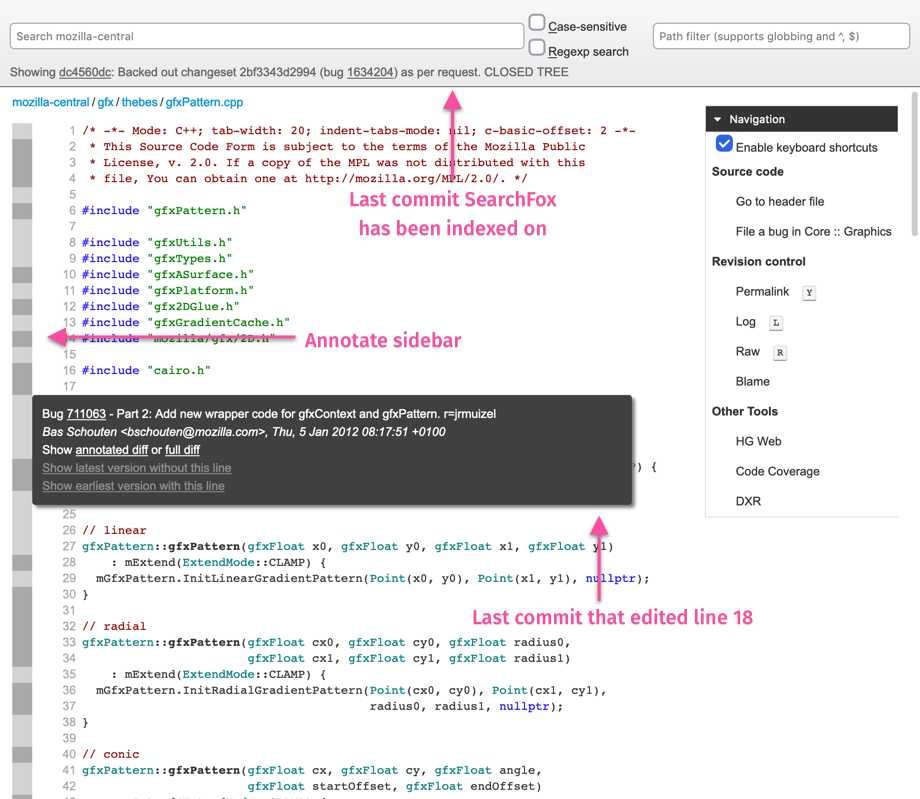
\includegraphics[width=\textwidth]{images/file-view.png}
    \caption{Searchfox file view for \texttt{gfx/thebes/gfxPattern.cpp}}
    \label{fig:searchfox-file-view}
\end{figure}

The log link and the annotate sidebar are particularly useful to understand why a piece of code 
was written in a certain way, especially since both of these contain references to the associated
Bugzilla issues where comments from the author or the reviewer can be found.

\section{Committing the changes}

Once the changes have been are tested, they should be committed to be sent for review.
This is done using the command below:

\begin{verbatim}
hg commit -m "Bug XXX - Commit message. r=reviewer"
\end{verbatim}

\noindent where:
\begin{itemize}
    \item \texttt{XXX} is the issue number on Bugzilla.
    \item ``Commit message'' is a sentence summarising the changes.
    \item the reviewer is referred to by their nickname.
\end{itemize}

Subsequent changes to the same revision can be done by amending the commit:
\begin{verbatim}
hg commit --amend
\end{verbatim}

If the commit is out of date, it is possible to update it by pulling the latest
source code using \texttt{hg pull}, then by rebasing the commit on top of the
central branch using \texttt{hg rebase -d central}.

\section{Submitting for review}

Mozilla uses a third-party tool called Phabricator \cite{phabricator}
for code reviews. This process is analogous to pull requests on Github. Mozilla's instance of Phabricator \cite{phabricator-moz} is integrated with a set of in-house tools:

\begin{itemize}
    \item \texttt{moz-phab}: a command-line utility to publish commits to Phabricator.
    \item Bugzilla integration bot, linking Bugzilla issues with Phabricator revisions.
    \item A code review bot that runs on every submitted revision and adding automated.
review comments from linters.
    \item Lando: a tool that allows merging the revision once it is accepted.
\end{itemize}

In order to submit a commit for review, it is necessary to have a Bugzilla account
to login to Phabricator. Once logged into Phabricator, assuming the commit to be submitted is already checked out, submitting for review can be done using the \texttt{moz-phab submit} command.

The commit is now submitted for review. Subsequent changes to address comments from
reviewers should be amended to the commit using \texttt{hg commit --amend} and re-submitted using
\texttt{moz-phab submit}.

\section{Testing}

To ensure changes work correctly and do not break existing features, it is necessary to perform
testing on the software. Manual testing can be done by the developer by running the compiled build of Firefox.
However, for complex software like Firefox, there are a lot of tasks that need to be tested, 
so manual testing would take a large amount of time. This is where automated tests become useful.

There are many types of tests in Firefox, but for the sake of simplicity, only the ones relevant to
this project will be described.

\subsection{Mochitests}

Quoted from the ``Mochitest'' Mozilla Developer Network page \cite{mochitest}:

\begin{quote}
Mochitest is an automated testing framework built on top of the MochiKit JavaScript libraries. It is an automated regression testing framework used by Mozilla to report success or failure to the test harness using JavaScript function calls.

Mochitest's use of JavaScript function calls to communicate test success or failure can be unsuitable for certain types of test. Only things that can be tested using JavaScript (with privileges!) can be tested with this framework. Given some creativity, that's actually much more than you might first think, but it's not possible to write Mochitest tests to directly test a non-scripted C++ component, for example.  (Use a compiled-code test to do that.)
\end{quote}


The main command to run mochitests is simply:
\begin{verbatim}
./mach mochitest
\end{verbatim}

This runs all the mochitests, taking a big amount of time, but using different parameters, it can run only a subset of tests if needed.

No new mochitests will be added in this project, only pre-existing ones will be edited to add new test cases (usually one or two lines) to cover conic gradients.

\subsection{Reference testing}

Reference tests, also referred to as reftests, are automated tests that ensure the rendering of a certain testcase is correct. A reference test is composed of two files: the test and the reference. Both files contain code that should render the same way. The test file uses the feature that is being tested, while the reference file does not. If both files render the same, the test passes. If not, the test fails \cite{reftests}. However, it is possible to allow a certain amount of difference by specifying the maximum number of different pixels and the maximum color channel (red, green or blue) difference in the test metadata. This is usually done when the difference is not directly due to the feature being tested, like a difference in how the graphics card handles both files \cite{reftests-fuzzy}.

When a test fails, the test log will include links to a screenshot of both the reference and the test files. They can be compared by pasting the logs into the reftest analyser tool \cite{reftest-analyser}, which can highlight where the pixels differ.

The following example is the reftest analyser highlighting differences between a test rendered locally and a png reference rendered on different hardware. There are 220 differing pixels, but differences are only by 1 in the color channels.

\begin{figure}[H]
    \centering
    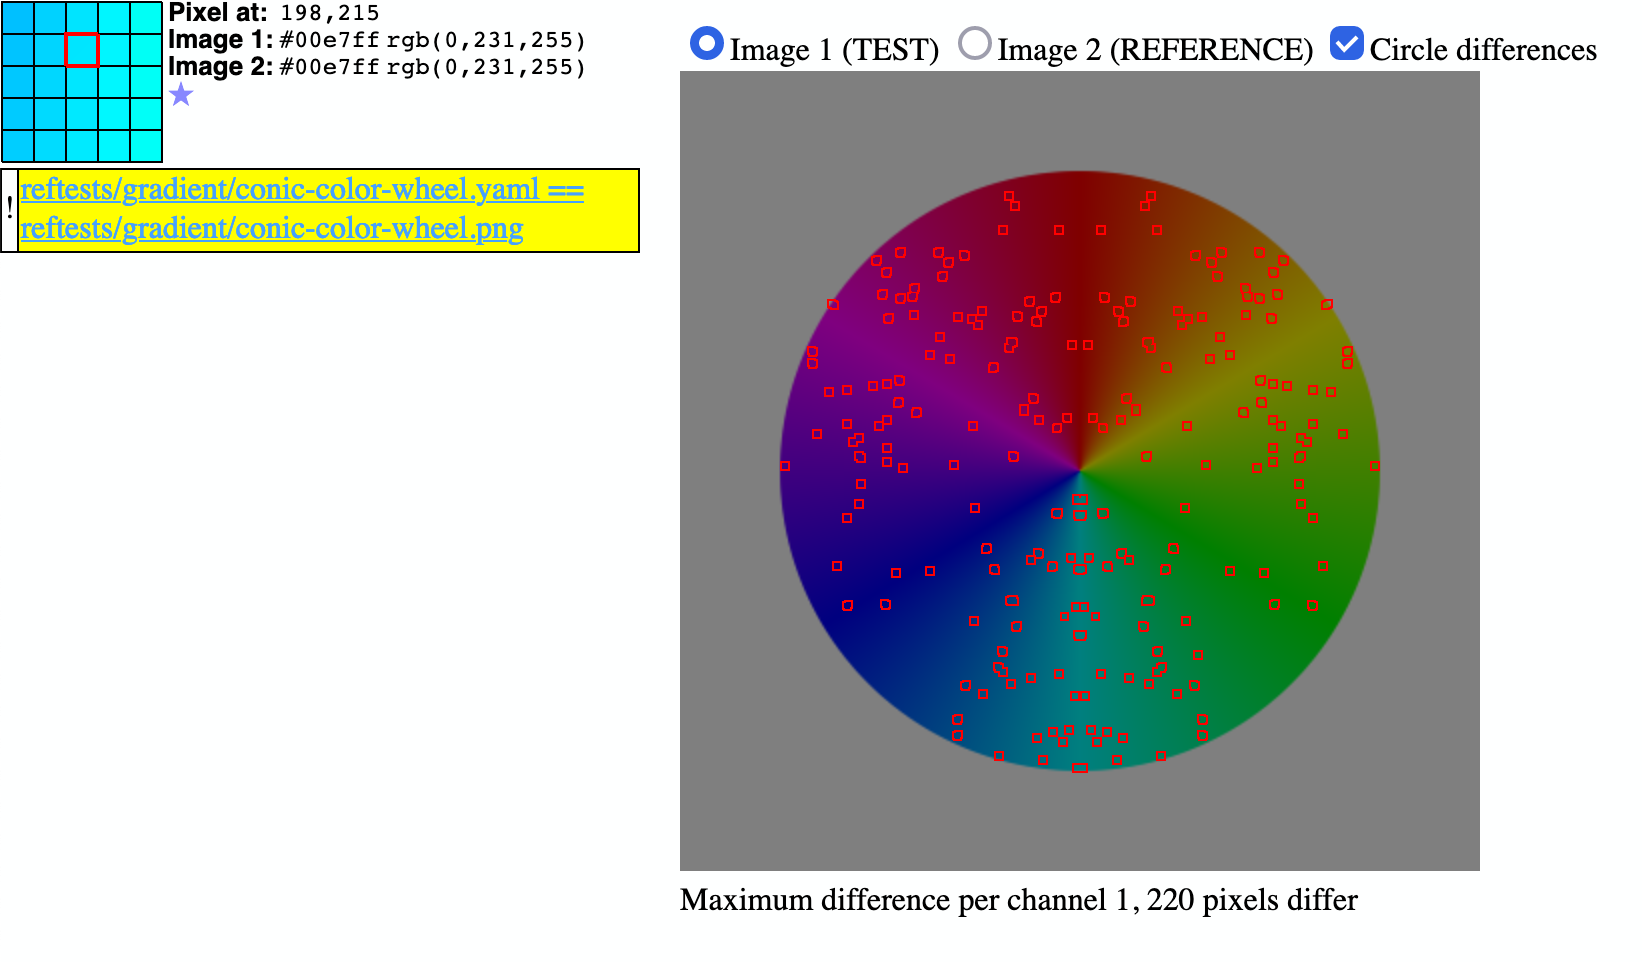
\includegraphics[width=\textwidth]{images/reftest-analyser.png}
    \caption{Reftest analyser}
    \label{fig:reftest_analyser}
\end{figure}

The \texttt{./mach reftest} command can run most types of reftests, but WebRender reftests need to
be run with \texttt{cargo run -- -p 1 reftest} since they use different toolchains.

Reference testing is central to this project since most of the testing that will be added is visual. This project will add two types of reftests: Wrench and Web Platform Tests reference tests, which will be described in their respective sections.

\subsection{The Try server}
While it is possible to run tests locally, it is not possible to perform other tasks on the computer while waiting, since some tests require the test window to stay focused all the time. There are also many tests and many different supported configurations (different platforms, preferences, etc.), that it would take hours to run everything.
To make it easier to execute entire test suites, Mozilla provides a ``Try'' server, where commits can be pushed as often as wanted and where tests will be ran on Mozilla's machines \cite{using-try}. To use it, level 1 commit access must be requested, by filing an issue with the SSH public key attached, then by finding someone to vouch for access (usually the mentor of the task) \cite{configuring-try}.

Once level 1 commit access is acquired, it is possible to use the following command:
\begin{verbatim}
./mach try chooser
\end{verbatim}

This will bring up a web page:
\begin{figure}[H]
    \centering
    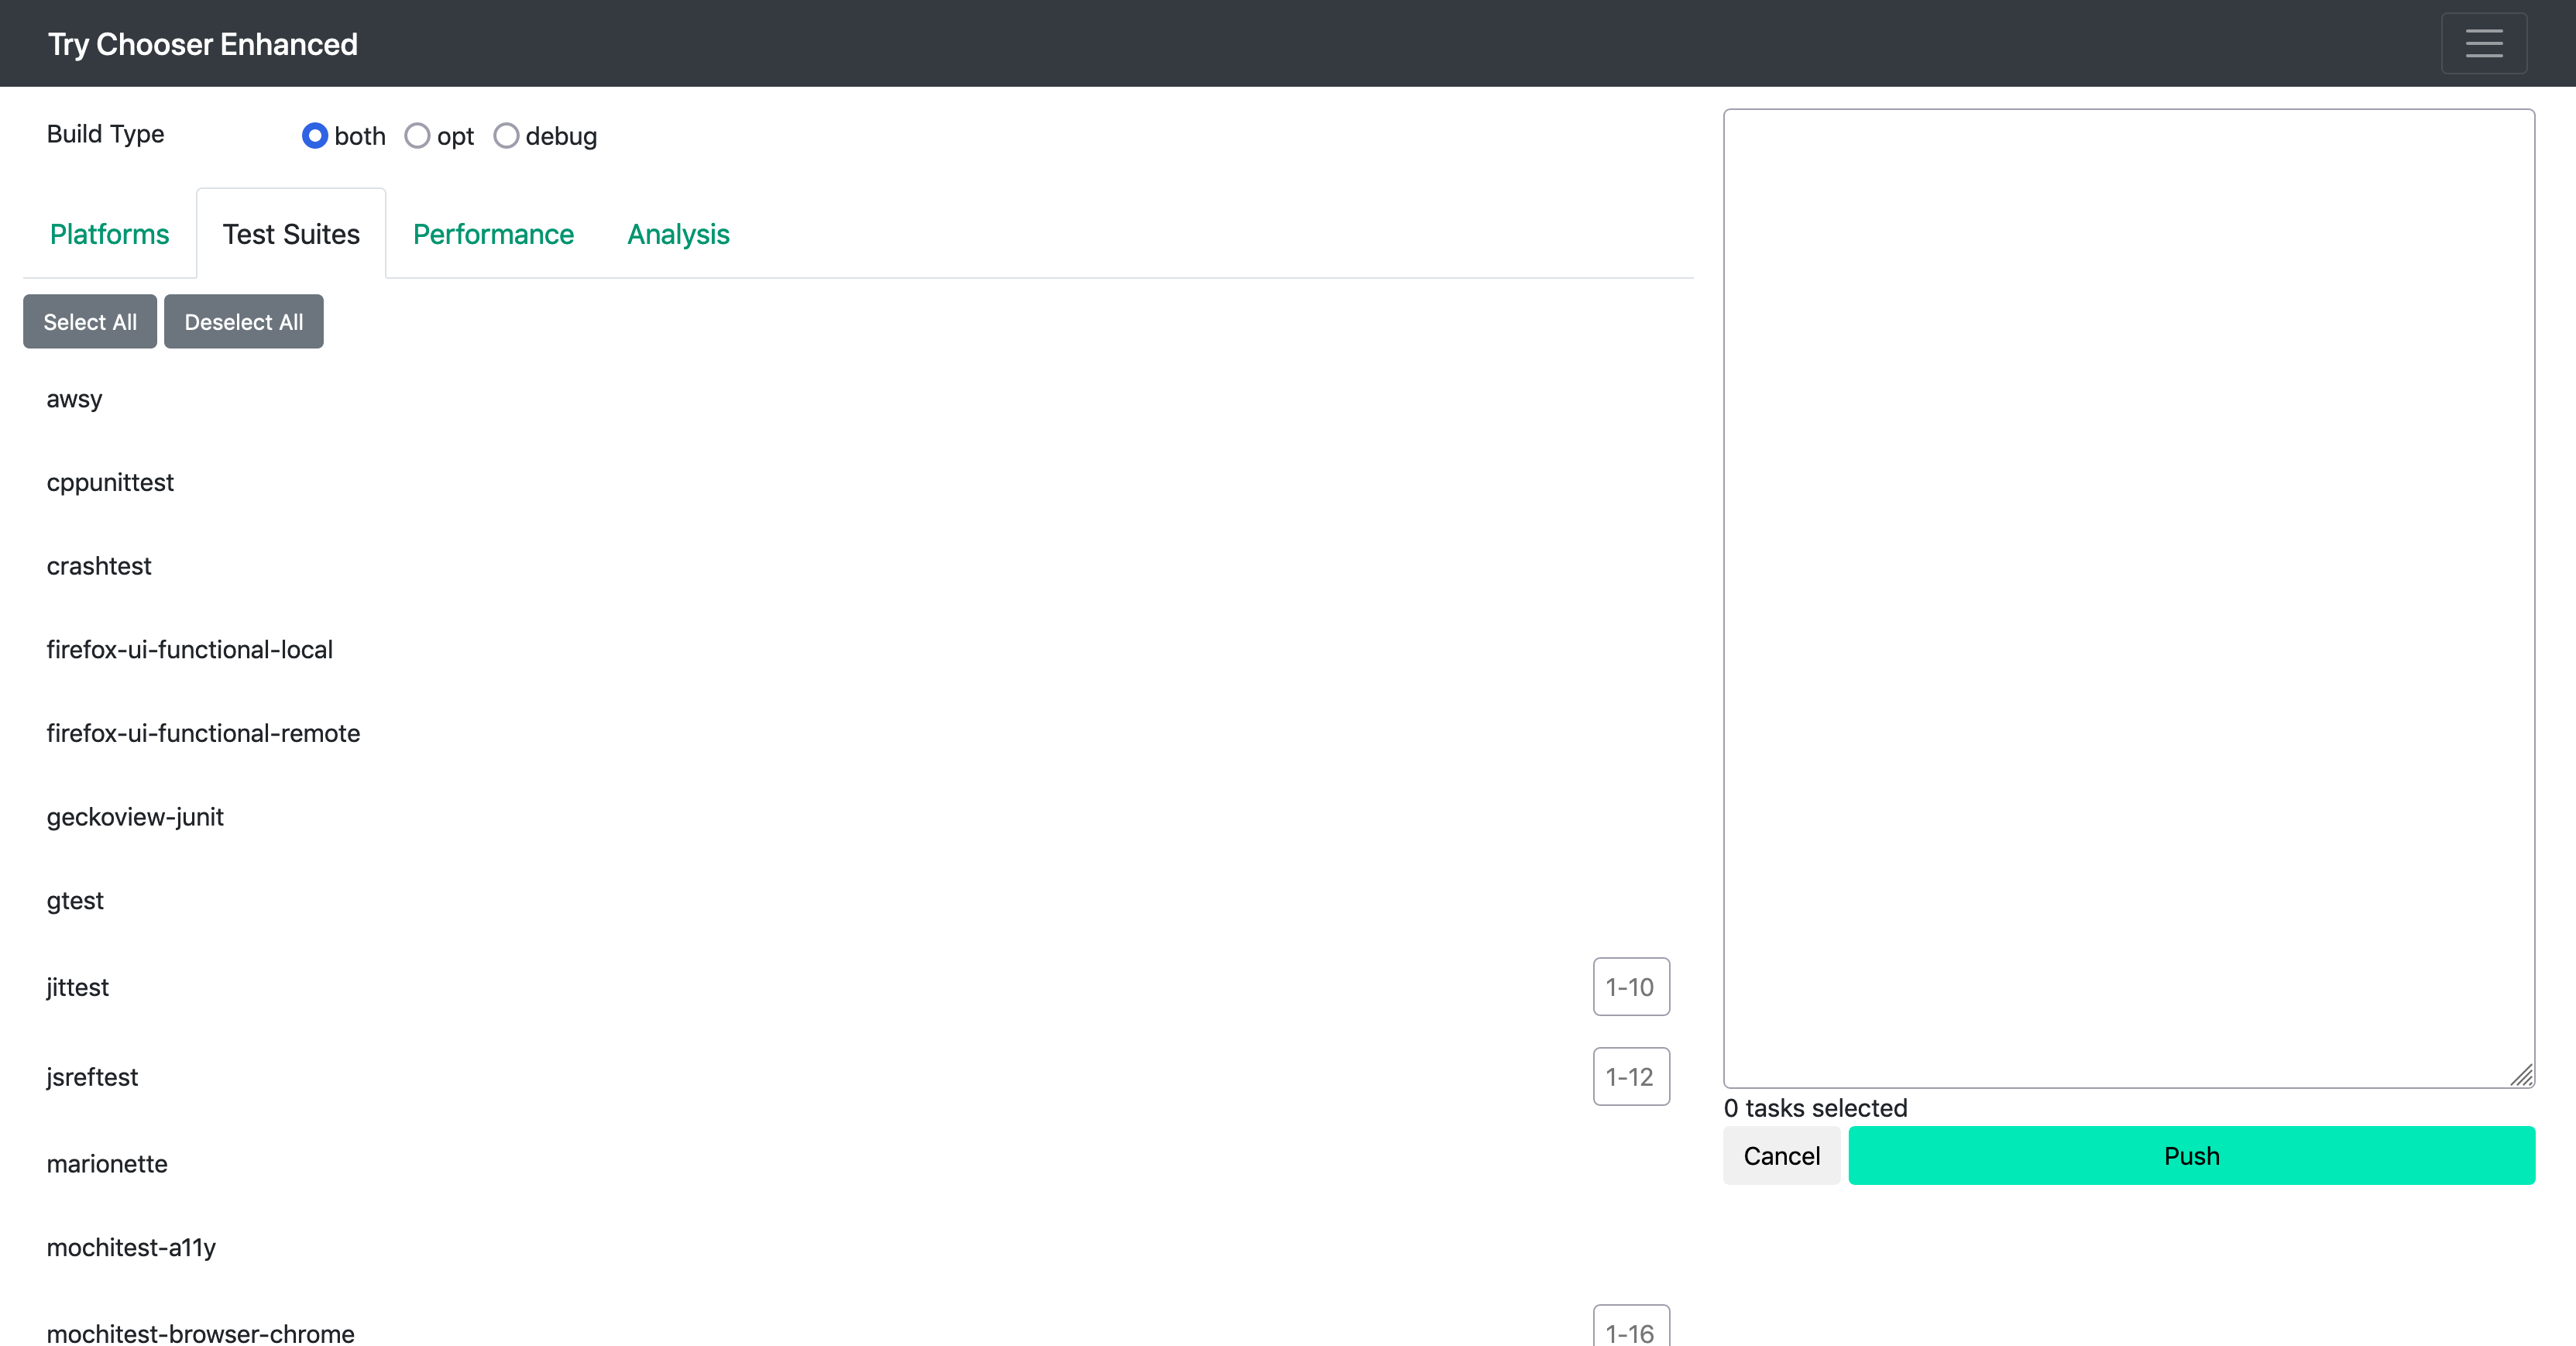
\includegraphics[width=\textwidth]{images/try-chooser.png}
    \caption{Try chooser}
    \label{fig:try_chooser}
\end{figure}

Different jobs/tasks/test suites and platforms can be selected and then pushed. A link will be provided in the command output to a tool called ``Treeherder'' \cite{treeherder} where test results can be checked after they are finished running. Here is a screenshot of the tool:

\begin{figure}[H]
    \centering
    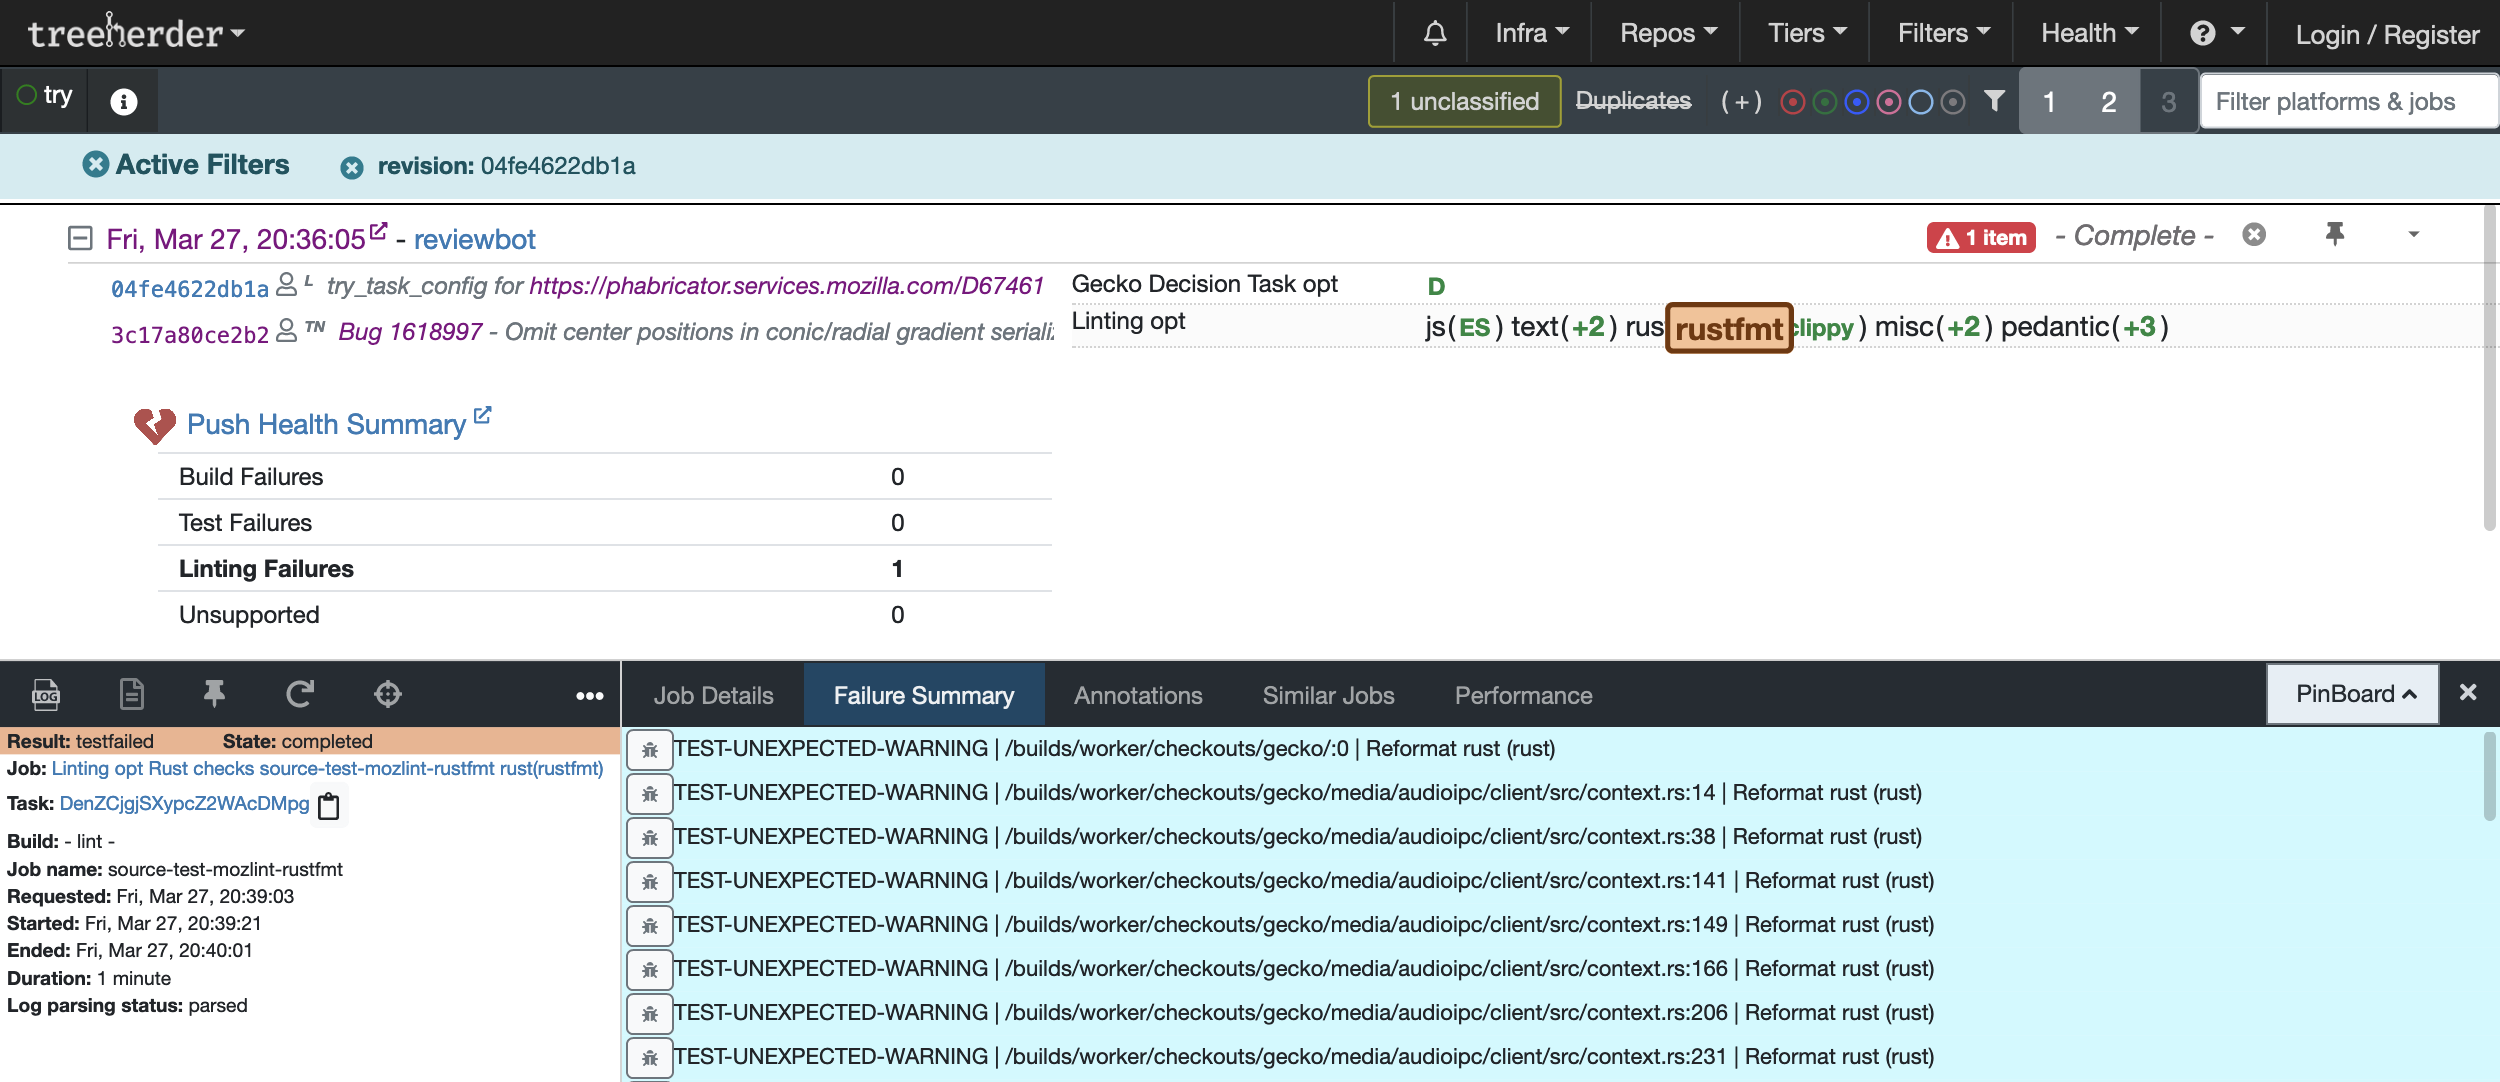
\includegraphics[width=\textwidth]{images/treeherder.png}
    \caption{Treeherder}
\end{figure}

From the top, the first toolbar is the navigation bar, which contains links irrelevant to the try push. On the second toolbar, the following elements can be seen:
\begin{itemize}
    \item The left side has the name of the repository (``try'' in this case, since it is the try server where the commit is being pushed to)
    \item From left to right, buttons in the right side filter different jobs based on the status (fail, success, etc.), the importance or the platform or job names. 
\end{itemize}

In the content area, the left side has the commits being pushed, while the right side displays the different jobs, color-coded based on the status. When a job is selected (``rustfmt'' in this case), the bottom pane shows up with more details about it:

\begin{itemize}
    \item The left sidebar has a toolbar with different actions to perform, relevant ones being ``view logs'' and ``re-trigger job'' (which may be useful to check whether a failure is intermittent or not). The job metadata is displayed under the toolbar.
    \item The right pane displays the logs, giving clues on why the job is failing.
\end{itemize}

\section{Merging the change}

When the revision is approved, the commit can be queued for check-in, using the ``Check-in Needed'' tag on Phabricator. The commit is then merged to the integration branch called ``autoland'', where all test suites run on Mozilla's machines. This process is analogous to continuous integration in other projects and results can be shown in the Treeherder UI decribed previously. If the commit causes a test failure, it is reverted from the integration branch. If there is no issue, the commit is merged along with other successful commits into the mozilla-central repository. The people taking care of manually doing the merges and reverting faulty commits are called ``sheriffs''.

mozilla-central contains the latest source code that is built twice a day by Mozilla's integration server into Firefox Nightly \cite{nightly}, the alpha version of Firefox, equivalent to Google Chrome Canary.

Every 4 weeks (previously 6 to 8 weeks) following a release calendar \cite{release-calendar}, the source code from mozilla-central is merged to mozilla-beta (the source code for Firefox Beta), and mozilla-beta is merged to mozilla-release (the source code for Firefox). After this merge, the version number is incremented for all 3 repositories. This work is done by the sheriffs, the release engineering and release management teams. There is a 4-day period before that merge date, called the soft freeze, where risky changes should be avoided and held for the next release.

For enterprises, Firefox has a yearly release called ``extended supported release'' (ESR) which is a version that only receives security updates for one year. It is in the mozilla-esrXX repository, where XX is the version number, and is merged from mozilla-release every year \cite{release-calendar}.

Sometimes, changes can be merged directly to the mozilla-beta, mozilla-release, mozilla-esrXX repositories if they are critical, with approval from release managers.

% -----------------------------------------------------------------------------

\chapter{Technical background}
\label{chap:technical}

\section{C++ and Rust}

There are two programming languages used by the Firefox rendering engine, Gecko: C++ and Rust. C++ is similar to C with more features for object-oriented programming, like classes or interfaces. It suffers from the same memory safety issues as C, such as buffer overflows due to using the same memory paradigms.

Rust is a low-level programming language developed by Mozilla in 2010 \cite{rust-creation}, although it has since developed its own independent community. Its main goal is to address the shortcomings of C++ in terms of memory safety \cite{rust}. It is mainly an imperative programming language and provides features familiar to C developers such as structs or enums. However, it also provides object-oriented programming features such as traits, which are similar to interfaces. Functional programming features such as pattern matching or lambdas can also be found.

The Firefox code makes use of \texttt{cbindgen} to make Rust code interact with C++ in the source code. It does this by generating C++ bindings that can be used directly from C++ code.

\section{Anatomy of a browser engine}
In order to describe the implementation, it is useful to first provide an in-breadth overview of
how a browser rendering engine renders web pages. This happens in 5 main steps, which are roughly similar for all 3 major rendering engines. Most of the contents in this section are summarised from Lin Clark's Code Cartoons blog post \cite{code-cartoons}.

The first step is parsing, HTML and CSS files are parsed into data structures that are understood by the rendering engine. The structures representing HTML are referred to as the DOM (Document Object Model). For this project, only CSS parsing is relevant and it is done by the style system.

The second step is styling. The CSS engine figures out which CSS properties should apply to each element on the web page, for which the process is not relevant to the project. Also, in each CSS property, since the initial value specified by the file may contain variables, different units or calculation functions, that value needs to be normalised into a final value, called the computed value.
An example would be \texttt{calc(45deg - 1turn)} being computed to \texttt{-315deg}.
The way normalisation should be done is not precisely specified by the CSS specification, meaning
that different browser engines can differ to this regard by doing what is convenient for them. The
only guideline given by the specification is to try to normalise to a value as short as possible.

The third step is layout. The rendering engine computes the on-screen size and position of each box on the webpage. Boxes can be elements in the HTML document, but also parts of those
elements such as lines of text or list markers. This part is not very relevant to the project,
since conic gradients don't affect the size or position of boxes on the screen.

The fourth step is painting. Each box is painted using the styling and layout information computed
at previous steps. The painting is potentially done on different layers, making it possible to repaint a single layer independently. 

The last step is rendering, which is essentially taking the layers from the previous step and
rendering them as one single image. Some CSS properties only are applied at this step, such as
\texttt{transform} (which performs translations, rotations and some other transforms),
or \texttt{animation}, since it is more convenient and performant for the browser engine to do so.


In Gecko, Firefox's rendering engine, the rendering step is fairly complicated, because Gecko has multiple graphics backends, which will be detailed in their respective implementation section. APIs are used to abstract away different backends. Although in the future, the plan is to replace all existing backends with WebRender. Here is a rough diagram representing the rendering flow:

\begin{figure}[H]
    \centering
    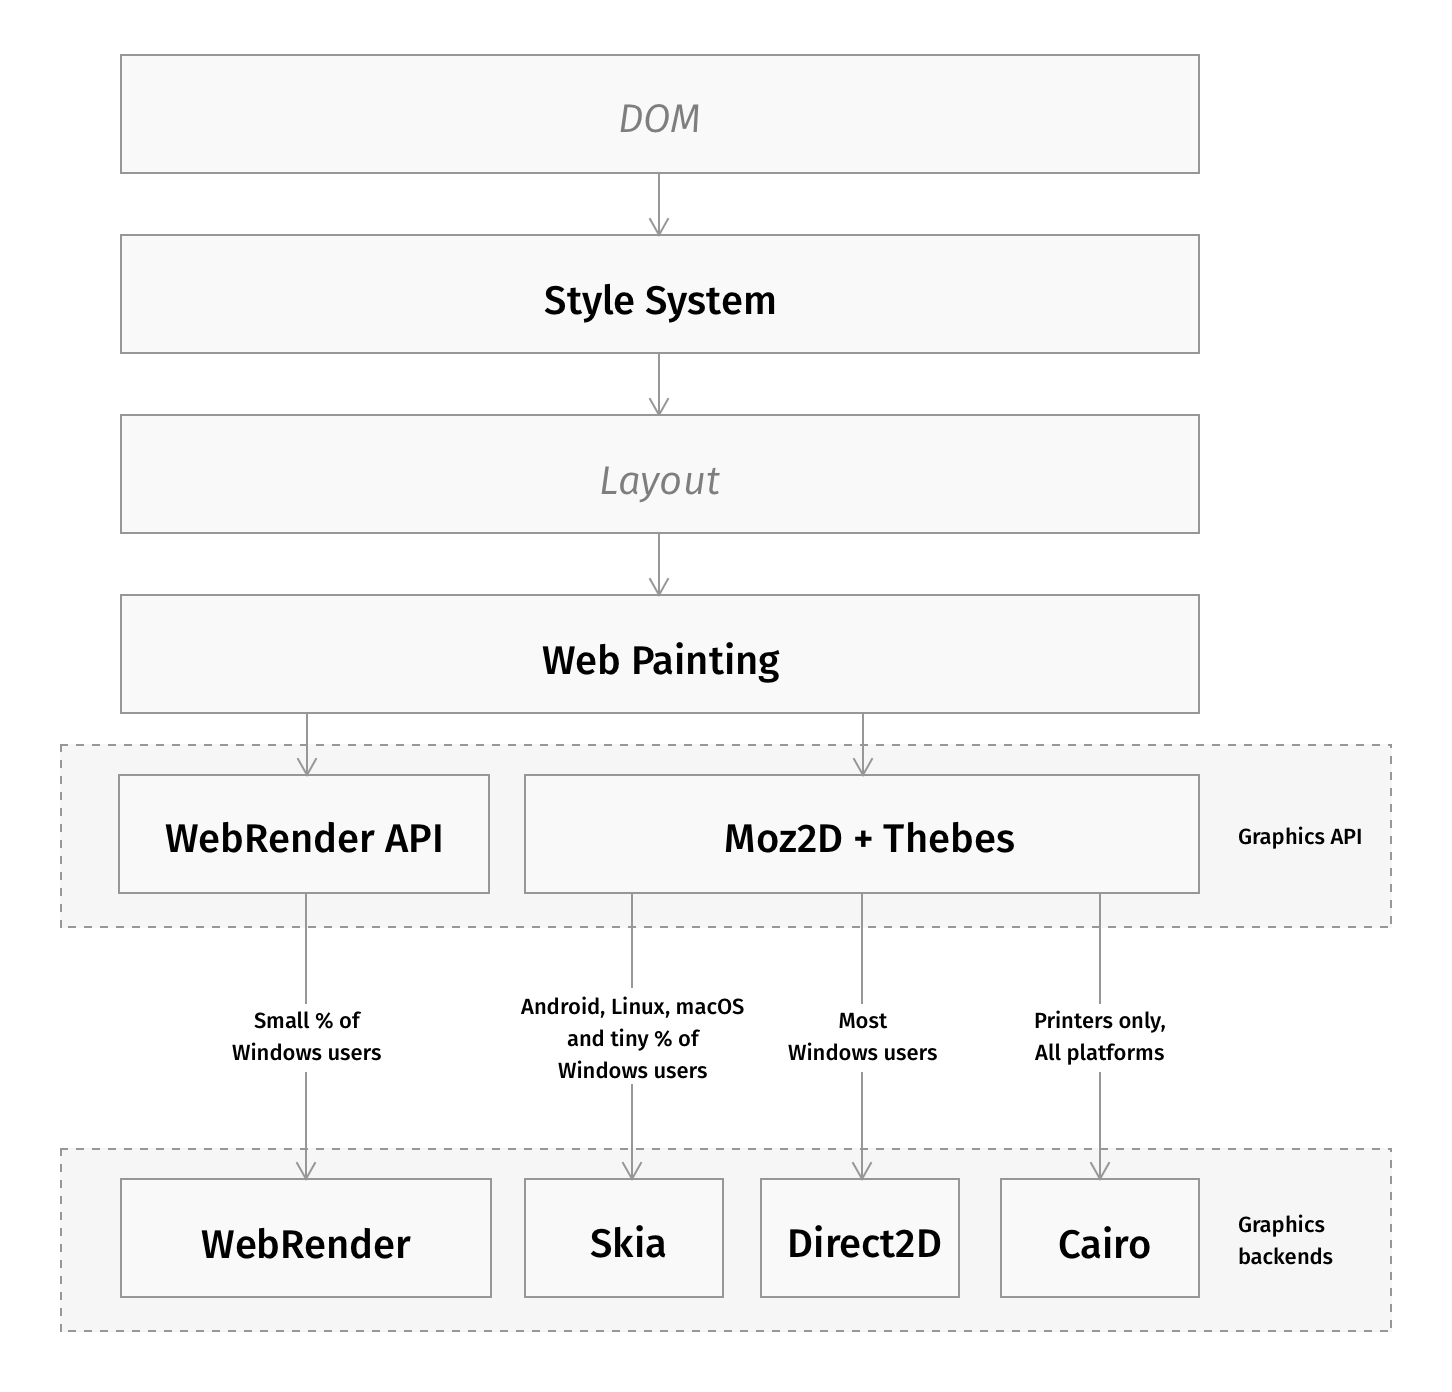
\includegraphics[width=0.9\textwidth]{images/diagram-gecko.png}
    \caption{How rendering works in Gecko}
    \label{fig:diagram-gecko}
\end{figure}

The grayed out boxes are steps untouched by this project.

\section{Shaders}

For the WebRender implementation, it is useful to describe what a graphics shader is. When doing computer graphics, shaders are programs that run at different points of the rendering pipeline, usually on the GPU \cite{shader-definition}. They are often used in computer games or in cinema post-processing. WebRender uses the ``OpenGL Shading Language'' for its shaders, also abbreviated as as GLSL \cite{webrender-readme}.

There are many different types of shaders but this section will only cover types relevant to this project: fragment shaders and vertex shaders.

Fragments are regions of the 3D scene that can render as one pixel on screen. The fragment shader runs for each fragment of the scene, with the properties of the fragment as input and the color of the pixel as output. \cite{fragment-shader}

The vertex shader, on the other hand, is ran once for each of the vertices. It is used to compute the position and data of anything related to the vertex \cite{vertex-shader}. Since it is ran less often than the fragment shader, it is usually good practice to pre-compute vertex data in there when possible.

The following diagram, taken from the open.gl website \cite{open-dot-gl-website}, is a good illustration of the graphics pipeline:

\begin{figure}[H]
    \centering
    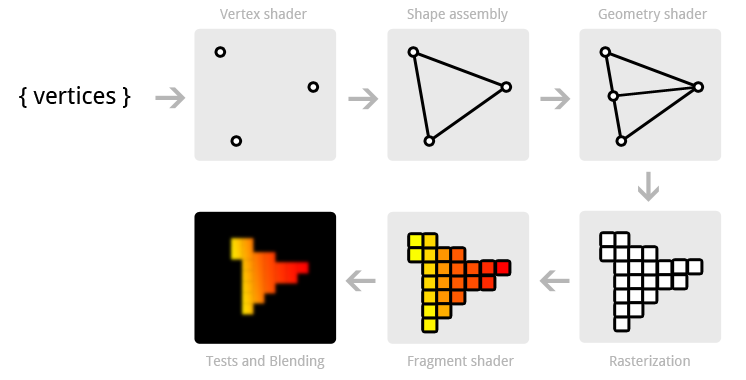
\includegraphics[width=\textwidth]{images/gfx-pipeline.png}
    \caption{Graphics pipeline}
    \label{fig:gfx-pipeline}
\end{figure}


% -----------------------------------------------------------------------------

\chapter{Implementation}
\label{chap:execution}


This section will describe the implementation done in Gecko, ordered by topic. For historical purposes, the list of merged commits related to this project can be found in appendix \ref{appx:list-of-commits}.

\section{Style System}
The CSS engine in Gecko taking care of the styling step is mostly written in Rust. Most of it is shared with the Servo browser engine, an experimental browser engine by Mozilla, also written in Rust \cite{servo}.
The code is located in the \texttt{servo/components/style/} directory.

The part handling CSS values, located in the \texttt{servo/components/style/values} directory, is split in multiple directories, for which three are directly relevant to this project:
\begin{itemize}
    \item \texttt{generics}: This directory defines the generic interfaces used by the other directories. Class names in this directory may be prefixed with \texttt{Generic}.
    \item \texttt{specified}: This directory contains the implementation for specified values (values specified by the developer) as defined in the specification \cite{specified-value}  and has the code for parsing those values.
    \item \texttt{computed}: This directory contains the implementation for computed values, which are the specified values with different types normalised and calculations resolved  \cite{computed-value}.
\end{itemize}{}

\noindent There are also two directories not directly relevant to this project:
\begin{itemize}
    \item \texttt{resolved}: The resolved CSS value is the value returned by the \texttt{getComputedStyle()} function. Most of the time, it is the computed value, but there are some special cases for web compatibility \cite{resolved-value}. For the \texttt{conic-gradient} case, while colors have a different resolved value, that bit was already implemented for other color-related properties, so no more work on resolved values is needed.
    \item \texttt{animated}: This directory defines types for animations and transitions. Image values like \texttt{conic-gradient} cannot be animated or transitioned \cite{unanimatable-images}, so no work is needed for this directory.
\end{itemize}{}


There is some pre-existing code handling gradients, for linear and radial gradients, that
was re-usable. However adding in conic gradients to the style system was not a simple task due to numerous differences that conic gradients have.


\subsection{Adding the AngleOrPercentage type}

The first of these differences is the need to support angles or percentages for color stop positions. Since no other CSS feature currently uses \texttt{<angle-percentage>}, the \texttt{AngleOrPercentage} type needed to be added to the style system. The complete diff can be viewed on Phabricator \cite{diff-angleOrPercentage}.

\subsubsection{Naming}

The name \texttt{AnglePercentage} was ruled out even though \texttt{<length-percentage>} is named \texttt{LengthPercentage} in the source code, since \texttt{AngleOrPercentage} does not support mixing angles and percentages in the \texttt{calc} CSS function, while \texttt{LengthPercentage} does support mixing lengths and percentages. An example of mixing angles and percentages is:

\begin{minted}{css}
conic-gradient(red calc(10deg + 25%), gold)
\end{minted}

While the specification says that this should be supported \cite{mixing-percentages}, from manual testing, no other web browser currently supports it (see appendix  \ref{appx:unsupported-angle-percentage}). Also, the use cases for mixing angles and percentages is low, since the above angle could be expressed as \texttt{calc(10deg + 90deg)} or directly as \texttt{100deg}. It is also not trivial to support, so this was left out for the initial implementation.

\subsubsection{Definition}

The implementation for \texttt{AngleOrPercentage}, both for the computed and specified versions, consists of a Rust enum saying it is either a \texttt{Percentage} or an \texttt{Angle}, and includes methods on top that re-use code from the two sub-types.

\begin{minted}{rust}
pub enum AngleOrPercentage {
    Percentage(Percentage),
    Angle(Angle),
}
\end{minted}

\subsubsection{Specified value implementation}

The specified value implementation contains the parsing code. The \texttt{parse\_internal} function does the following:
\begin{enumerate}
    \item Try to parse the value as a percentage
    \item Return that percentage value if successful
    \item Try to parse the value as an angle value
\end{enumerate}

There is a \texttt{parse\_with\_unitless} and a \texttt{parse} function which both call the \texttt{parse\_internal} function with a different ``allow unitless zero'' parameter. The distinction is subtle, but the parameter determines whether to allow \texttt{0} without any unit. Even though zeroes without units are convenient, they are ambiguous just like any unitless number, especially for properties that accept multiple numeric values as full value. As an example, the relevant \texttt{csswg-drafts} Github issue \cite{unitless-zeroes-issue} uses the \texttt{offset} CSS property value, defined as:
\begin{verbatim}
[ offset-position? [ offset-path [ <length-percentage> || offset-rotate ]? ]? ]!
[ / offset-anchor ]?
\end{verbatim}

\noindent where \texttt{offset-rotate} is \texttt{[ auto | reverse ] || <angle>}.

A value like \texttt{offset: ray(180deg) 0;} (where \texttt{ray(180deg)} is \texttt{offset-path}) then becomes ambiguous since \texttt{0} could be either the \texttt{<length-percentage>} or the \texttt{offset-rotate} value. It was decided in that Github issue that unitless zeroes should only be allowed for CSS transforms, filters, gradients for compatibility reasons. 

As for conic gradients, the specification explicitly says unitless zeroes should be allowed for color stop positions \cite{unitless-zeroes-conic-gradient}, presumably for consistency with other gradients. However, the default parsing method for \texttt{AngleOrPercentage} remains without unitless zero support to avoid accidentally supporting it for future specifications using this type.

\noindent The full code for the specified value implementation can be found in appendix \ref{appx:specified-angle-or-percentage}.

\subsubsection{Computed value implementation}

The computed value implementation has two methods from the \texttt{ToComputedValue} trait:

\begin{itemize}
    \item \texttt{to\_computed\_value}, which resolves a specified value to a computed value.
    \item \texttt{from\_computed\_value}, which reconstructs a specified value from a computed value.
\end{itemize}

\noindent Both of these methods pattern match on the value then call pre-existing methods from the sub-types:

\begin{minted}{rust}
impl ToComputedValue for specified::AngleOrPercentage {
    type ComputedValue = AngleOrPercentage;

    #[inline]
    fn to_computed_value(&self, context: &Context) -> AngleOrPercentage {
        match *self {
            specified::AngleOrPercentage::Percentage(percentage) => {
                AngleOrPercentage::Percentage(percentage.to_computed_value(context))
            },
            specified::AngleOrPercentage::Angle(angle) => {
                AngleOrPercentage::Angle(angle.to_computed_value(context))
            },
        }
    }
    #[inline]
    fn from_computed_value(computed: &AngleOrPercentage) -> Self {
        match *computed {
            AngleOrPercentage::Percentage(percentage) => {
                specified::AngleOrPercentage::Percentage(ToComputedValue::from_computed_value(
                    &percentage,
                ))
            },
            AngleOrPercentage::Angle(angle) => {
                specified::AngleOrPercentage::Angle(ToComputedValue::from_computed_value(&angle))
            },
        }
    }
}
\end{minted}

\subsection{Refactoring gradient code}
\label{refactor-gradient-code}

Once the \texttt{AngleOrPercentage} type was added, the existing gradient implementation needed to be more generic to allow using this type instead of \texttt{LengthPercentage}. To do this, instances of \texttt{LengthPercentage} were first replaced with Rust generic types \cite{generic-types}, in the \texttt{ColorStop} and \texttt{GradientItem} implementations. These pre-existing classes are respectively analogous to the \texttt{<color-stop>} type and the type of \texttt{<color-stop-list>} items, both from the CSS Images specification \cite{color-stop-spec}.

To illustrate the change, here is an extract from the full diff \cite{diff-generic-types}:

\begin{minted}{diff}
--- a/servo/components/style/values/generics/image.rs
+++ b/servo/components/style/values/generics/image.rs
@@ -175,48 +175,48 @@ pub enum ShapeExtent {
-pub enum GenericGradientItem<Color, LengthPercentage> {
+pub enum GenericGradientItem<Color, T> {
     /// A simple color stop, without position.
     SimpleColorStop(Color),
     /// A complex color stop, with a position.
     ComplexColorStop {
         /// The color for the stop.
         color: Color,
         /// The position for the stop.
-        position: LengthPercentage,
+        position: T,
     },
     /// An interpolation hint.
-    InterpolationHint(LengthPercentage),
+    InterpolationHint(T),
 }
 
 pub use self::GenericGradientItem as GradientItem;
 
 /// A color stop.
 /// <https://drafts.csswg.org/css-images/#typedef-color-stop-list>
 #[derive(
     Clone, Copy, Debug, MallocSizeOf, PartialEq, ToComputedValue, ToCss, ToResolvedValue, ToShmem,
 )]
-pub struct ColorStop<Color, LengthPercentage> {
+pub struct ColorStop<Color, T> {
     /// The color of this stop.
     pub color: Color,
     /// The position of this stop.
-    pub position: Option<LengthPercentage>,
+    pub position: Option<T>,
 }
 
-impl<Color, LengthPercentage> ColorStop<Color, LengthPercentage> {
+impl<Color, T> ColorStop<Color, T> {
     /// Convert the color stop into an appropriate `GradientItem`.
     #[inline]
-    pub fn into_item(self) -> GradientItem<Color, LengthPercentage> {
+    pub fn into_item(self) -> GradientItem<Color, T> {
         match self.position {
\end{minted}

This change was not sufficient, since the gradient type definition was split into two parts:
\texttt{Gradient} and \texttt{GradientKind}. \texttt{Gradient} contains information shared between all types of gradients, while \texttt{GradientKind} contains information specific to each gradient type (linear/radial), as shown below:

\begin{figure}[H]
    \centering
    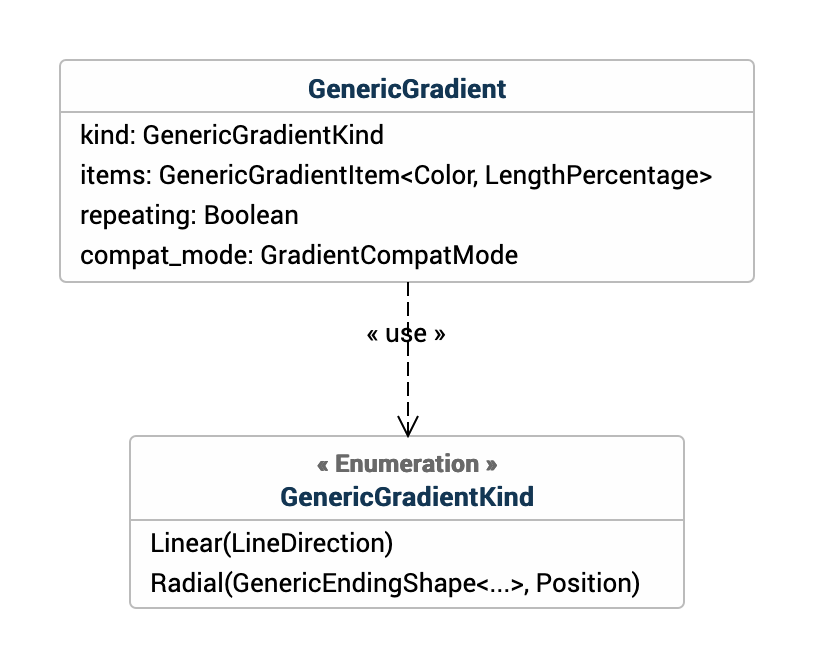
\includegraphics[width=300px]{images/class-diagram-before.png}
    \caption{Class diagram before refactor}
    \label{fig:class-diagram-before}
\end{figure}

Given that the \texttt{items} field would differ for conic gradients, due to using a different unit type, it would need to move to \texttt{GradientKind}, but that would leave only \texttt{repeating} and \texttt{compat\_mode} in the shared \texttt{Gradient} structure. 

As mentioned in chapter \ref{chap:context}, there are prefixes like \texttt{-moz-linear-gradient} or \texttt{-webkit-gradient} that need to remain supported, for which the parsing of the function can differ. These different parsing modes are represented via the compatibility mode. However, prefixes are not relevant to conic gradients, leaving only the \texttt{repeating} field shared between gradients. Hence, the \texttt{GradientKind} was merged back into \texttt{Gradient}. The new structure now looks like this:

\begin{figure}[H]
    \centering
    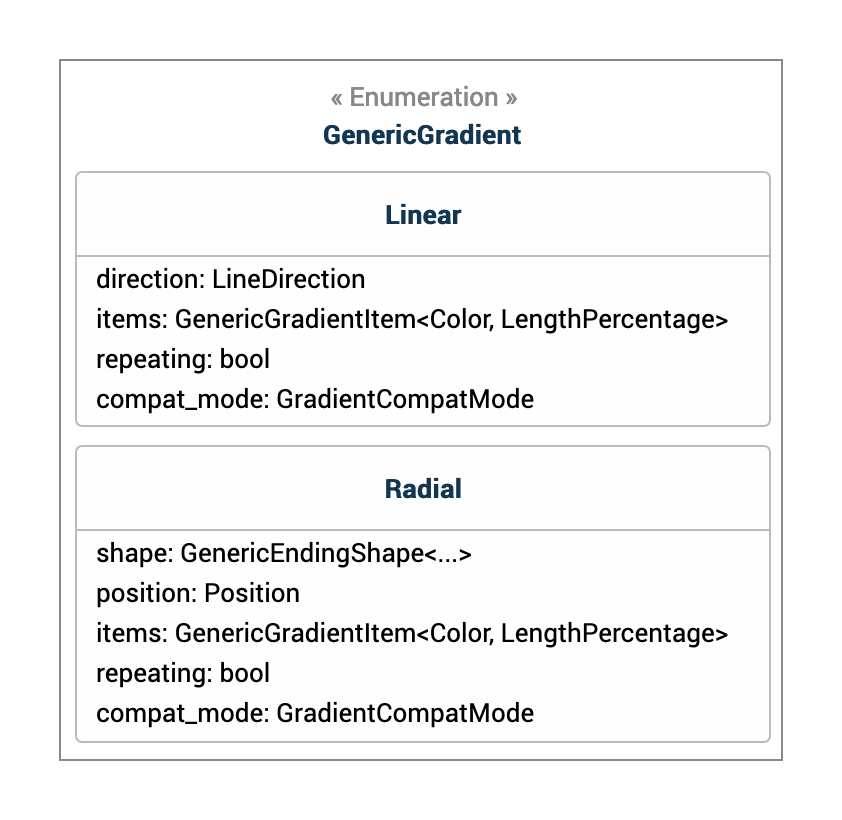
\includegraphics[width=300px]{images/class-diagram-after.png}
    \caption{Class diagram after refactor}
    \label{fig:class-diagram-after}
\end{figure}

Changing the structure required adapting most of the existing code in the style system. The web painting code (in C++), which uses those structures via \texttt{cbindgen}, also needed to be adapted. For instance, \texttt{aGradient.kind.AsRadial()} was changed to \texttt{aGradient.AsRadial()}.

The full definition of the structures can be found in appendix \ref{appx:refactoring-gradient-code} and the complete diff of the refactor can be viewed on Phabricator \cite{diff-refactor-style}.

\subsection{Parsing}

Now that the gradient implementation is generic enough, the conic gradient parsing can now
be implemented. First, the \texttt{Gradient} structure needs to be augmented to know what a
conic gradient is. The conic gradient type is defined below:

\begin{verbatim}
/// A conic gradient.
Conic {
    /// Start angle of gradient
    angle: Angle,
    /// Center of gradient
    position: Position,
    /// The color stops and interpolation hints.
    items: crate::OwnedSlice<GenericGradientItem<Color, AngleOrPercentage>>,
    /// True if this is a repeating gradient.
    repeating: bool,
},
\end{verbatim}

To support the \texttt{conic-gradient} and \texttt{repeating-conic-gradient} functions, cases need to be added to detect them, in the gradient \texttt{parse} function:

\begin{minted}{diff}
 let (shape, repeating, compat_mode) = match_ignore_ascii_case! { &func,
     // [...]
+    "conic-gradient" if static_prefs::pref!("layout.css.conic-gradient.enabled") => {
+        (Shape::Conic, false, GradientCompatMode::Modern)
+    },
+    "repeating-conic-gradient" if static_prefs::pref!("layout.css.conic-gradient.enabled") => {
+        (Shape::Conic, true, GradientCompatMode::Modern)
+    },
     // [...]
};
 Ok(input.parse_nested_block(|i| {
     Ok(match shape {
         // [...]
+        Shape::Conic => Self::parse_conic(context, i, repeating)?,
     })
 })?)
\end{minted}

\texttt{static\_prefs::pref!("layout.css.conic-gradient.enabled")} checks that the
feature flag is turned on. If it is turned off, conic gradients will be ignored.

Once the cases are handled, the \texttt{conic-gradient} parsing needs to be defined. The steps to parse the \texttt{conic-gradient} function are:
\begin{enumerate}
    \item Try to parse a \texttt{from} token followed by an angle, that is potentially an unitless zero.
    \item Try to parse an \texttt{at} token followed by a position.
    \item If an angle or a position was found, expect a comma.
    \item If not specified, use zero as the default angle, and center as default position
    \item Parse the color stops with angles or percentages as positions, and potentially unitless zeros
    \item Reject the function if there are less than 2 color stops (a gradient with 1 stop is pointless since it is just a solid color)
    \item Return a conic gradient structure
\end{enumerate}

\noindent The code for the parsing function can be seen below:
\begin{minted}[breaklines]{rust}
fn parse_conic<'i, 't>(
    context: &ParserContext,
    input: &mut Parser<'i, 't>,
    repeating: bool,
) -> Result<Self, ParseError<'i>> {
    let angle = input.try(|i| {
        i.expect_ident_matching("from")?;
        // Spec allows unitless zero start angles
        // https://drafts.csswg.org/css-images-4/#valdef-conic-gradient-angle
        Angle::parse_with_unitless(context, i)
    });
    let position = input.try(|i| {
        i.expect_ident_matching("at")?;
        Position::parse(context, i)
    });
    if angle.is_ok() || position.is_ok() {
        input.expect_comma()?;
    }

    let angle = angle.unwrap_or(Angle::zero());
    let position = position.unwrap_or(Position::center());
    let items = generic::GradientItem::parse_comma_separated(context, input, AngleOrPercentage::parse_with_unitless)?;

    if items.len() < 2 {
        return Err(input.new_custom_error(StyleParseErrorKind::UnspecifiedError));
    }

    Ok(Gradient::Conic {
        angle,
        position,
        items,
        repeating,
    })
}
\end{minted}


\subsection{Serialisation}

Now that the gradient is parsed into a structure that is understood by the style system, the style
system needs to be able to serialise the structure back to CSS if asked by the following JavaScript
methods: \texttt{getComputedStyle(element)} or \texttt{element.style}. To do this, the \texttt{ToCss}
Rust trait must be implemented for conic gradients. The method takes a gradient structure and 
transforms it back to a CSS string.

\begin{minted}{diff}
 fn to_css<W>(&self, dest: &mut CssWriter<W>) -> fmt::Result
 where
     W: Write,
 {
     // [...]
     match *self {
         // [...]
+        Gradient::Conic { ref angle, ref position, ref items, .. } => {
+            dest.write_str("conic-gradient(")?;
+            let omit_angle = angle.is_zero();
+            let omit_position = position.is_center();
+            if !omit_angle {
+                dest.write_str("from ")?;
+                angle.to_css(dest)?;
+                if !omit_position {
+                    dest.write_str(" ")?;
+                }
+            }
+            if !omit_position {
+                dest.write_str("at ")?;
+                position.to_css(dest)?;
+            }
+            let mut skip_comma = omit_angle && omit_position;
+            for item in &**items {
+                if !skip_comma {
+                    dest.write_str(", ")?;
+                }
+                skip_comma = false;
+                item.to_css(dest)?;
+            }
+        },
+    }
     dest.write_str(")")
 }
\end{minted}

Since the specification says CSS structures should be serialised to the most simple form when possible, the angle and the position are omitted if they use their default values \cite{serialization-shortest-form}. Although it was not a big issue, it is worth noting that the position was not omitted for radial gradients when it was using the default value (the center of the element), Chrome and Safari also do not respect this \cite{serialization-broken-chrome}. This was fixed in Firefox along with the conic gradient implementation \cite{serialization-fixed-firefox}. For instance, \texttt{radial-gradient(at 50\% 50\%, red, green)} now gets simplified to \texttt{radial-gradient(red, green)}.

To fix this for both conic and radial gradients, a new Rust trait named \texttt{PositionComponent} was defined in the \texttt{generics} directory. The trait contains a \texttt{is\_center} method, checking whether the position component (horizontal or vertical) is the central one:

\begin{minted}{rust}
/// Implements a method that checks if the position is centered.
pub trait PositionComponent {
    /// Returns if the position component is 50% or center.
    /// For pixel lengths, it always returns false.
    fn is_center(&self) -> bool;
}
\end{minted}

\noindent The following classes implement this trait:
\begin{itemize}
    \item \texttt{Position} in the \texttt{generics} directory, where the implementation checks whether both the horizontal and vertical components of the position are central.
    \item \texttt{LengthPercentage} in the \texttt{computed} directory, where the implementation converts the value to a percentage, then pattern matches against it.
    \item \texttt{PositionComponent} in the \texttt{specified} directory, for the \texttt{<position>} CSS type \cite{spec-position}, where the implementation pattern matches against the type of value used.
\end{itemize}

\noindent For instance, here is the implementation for the \texttt{LengthPercentage} class:

\begin{minted}{rust}
impl GenericPositionComponent for LengthPercentage {
    fn is_center(&self) -> bool {
        match self.to_percentage() {
            Some(Percentage(per)) => per == 0.5,
            _ => false,
        }
    }
}
\end{minted}

Now that this \texttt{PositionComponent} trait is implemented, using it in the conic gradient code consists of omitting the position if central, when serialising:

\begin{minted}{diff}
             Gradient::Conic { ref angle, ref position, ref items, .. } => {
                 dest.write_str("conic-gradient(")?;
-                if !angle.is_zero() {
+                let omit_angle = angle.is_zero();
+                let omit_position = position.is_center();
+                if !omit_angle {
                     dest.write_str("from ")?;
                     angle.to_css(dest)?;
-                    dest.write_str(" ")?;
+                    if !omit_position {
+                        dest.write_str(" ")?;
+                    }
                 }
-                dest.write_str("at ")?;
-                position.to_css(dest)?;
+                if !omit_position {
+                    dest.write_str("at ")?;
+                    position.to_css(dest)?;
+                }
+                let mut skip_comma = omit_angle && omit_position;
                 for item in &**items {
-                    dest.write_str(", ")?;
+                    if !skip_comma {
+                        dest.write_str(", ")?;
+                    }
+                    skip_comma = false;
                     item.to_css(dest)?;
                 }
             },
\end{minted}

As the code above shows, it is important to take extra care to avoid including the associated keyword (\texttt{from} or \texttt{at}) and whitespace if omitting the angle or position. It is also important to skip the first comma if both the angle and position are omitted, to prevent ending up with an invalid CSS value like \texttt{conic-gradient(, red, blue)}.

\noindent The full diff can be found on Phabricator for completeness \cite{serialization-fixed-firefox}.

\subsection{Testing}
Existing parsing and serialisation tests were augmented with testcases for correct syntax, but also for invalid syntax:
\begin{minted}{javascript}
/* Invalid units */
"conic-gradient(red, blue 50px, yellow 30px)",
"conic-gradient(from 0%, black, white)",
"conic-gradient(from 60%, black, white)",
"conic-gradient(from 40px, black, white)",
"conic-gradient(from 50, black, white)",
"conic-gradient(at 50deg, black, white)",
"conic-gradient(from 40deg at 50deg, black, white)",
"conic-gradient(from 40deg at 50deg 60deg, black, white)",
/* Invalid keywords (or ordering) */
"conic-gradient(at 40% from 50deg, black, white)",
"conic-gradient(to 50deg, black, white)",
/* Conic gradients should not support prefixed syntax */
"-webkit-gradient(conic, 1 2, 3 4, color-stop(0, lime))",
"-webkit-conic-gradient(red, blue)",
"-moz-conic-gradient(red, blue)",
"-webkit-repeating-conic-gradient(red, blue)",
"-moz-repeating-conic-gradient(red, blue)",
\end{minted}

\section{Web Painting}

Now that the gradient is parsed to a structure understood by the code, the painting phase needs to happen.

The web painting code is all in C++ and is in the \texttt{layout/painting/} directory. The relevant code for gradients is located in the \texttt{nsCSSGradientRenderer} class, and is used in \texttt{nsImageRenderer} class for all image related CSS properties (such as \texttt{background-image} or \texttt{mask-image}), except for \texttt{border-image} which \texttt{nsCSSBorderImageRenderer} handles. 

This code knows about the size and position of the element on the screen, which was not available in the style system. This allows some information like the position of the conic gradient to be resolved, which is needed for painting.

After the refactor mentioned in section \ref{refactor-gradient-code}, the \texttt{nsCSSRenderingGradients.cpp} file (containing \newline \texttt{nsCSSGradientRenderer}) was changed over multiple commits (listed in chronological order), for which the combined diff can be found in appendix \ref{appx:nsCSSRenderingGradients-changes}:

\begin{enumerate}
    \item Tim Nguyen - Bug 1615862 - Handle conic-gradients in nsCSSGradientRenderer for WebRender. r=emilio,mstange (\texttt{https://phabricator.services.mozilla.com/D63018})
    \item Tim Nguyen - Bug 1616587 - Implement conic-gradient for Skia graphics backend. r=lsalzman (\texttt{https://phabricator.services.mozilla.com/D63415})
    \item Tim Nguyen - Bug 1620328 - Set conic-gradient angle range on Skia. r=lsalzman \newline (\texttt{https://phabricator.services.mozilla.com/D65910})
\end{enumerate}

The first step was setting up the ground work for supporting conic gradients in both \texttt{nsCSSGradientRenderer} and \texttt{nsCSSBorderImageRenderer}:

\begin{itemize}
    \item Fields, variables and methods for properties specific to conic gradients (center and start angle) were added to the class.
    \item Extra cases were added where relevant.
\end{itemize}

The diff below shows an example of the above changes done on the \texttt{nsCSSGradientRenderer::Create} method:

\begin{minted}{diff}
 nsCSSGradientRenderer nsCSSGradientRenderer::Create(
     nsPresContext* aPresContext, ComputedStyle* aComputedStyle,
     const StyleGradient& aGradient, const nsSize& aIntrinsicSize) {
   auto srcSize = CSSSize::FromAppUnits(aIntrinsicSize);
 
   // Compute "gradient line" start and end relative to the intrinsic size of
   // the gradient.
-  CSSPoint lineStart, lineEnd;
-  CSSCoord radiusX = 0, radiusY = 0;  // for radial gradients only
+  CSSPoint lineStart, lineEnd, center;  // center is for conic gradients only
+  CSSCoord radiusX = 0, radiusY = 0;    // for radial gradients only
+  float angle = 0.0;                    // for conic gradients only
   if (aGradient.IsLinear()) {
     Tie(lineStart, lineEnd) =
         ComputeLinearGradientLine(aPresContext, aGradient, srcSize);
-  } else {
+  } else if (aGradient.IsRadial()) {
     Tie(lineStart, lineEnd, radiusX, radiusY) =
         ComputeRadialGradientLine(aGradient, srcSize);
+  } else {
+    MOZ_ASSERT(aGradient.IsConic());
+    Tie(center, angle) = ComputeConicGradientProperties(aGradient, srcSize);
   }
   // Avoid sending Infs or Nans to downwind draw targets.
   if (!lineStart.IsFinite() || !lineEnd.IsFinite()) {
     lineStart = lineEnd = CSSPoint(0, 0);
   }
+  if (!center.IsFinite()) {
+    center = CSSPoint(0, 0);
+  }
   CSSCoord lineLength =
       NS_hypot(lineEnd.x - lineStart.x, lineEnd.y - lineStart.y);
 
   // Build color stop array and compute stop positions
   nsTArray<ColorStop> stops =
       ComputeColorStops(aComputedStyle, aGradient, lineLength);
 
   ResolveMidpoints(stops);
@@ -672,16 +723,21 @@ nsCSSGradientRenderer nsCSSGradientRende
       aPresContext->CSSPixelsToDevPixels(lineStart.y),
   };
   renderer.mLineEnd = {
       aPresContext->CSSPixelsToDevPixels(lineEnd.x),
       aPresContext->CSSPixelsToDevPixels(lineEnd.y),
   };
   renderer.mRadiusX = aPresContext->CSSPixelsToDevPixels(radiusX);
   renderer.mRadiusY = aPresContext->CSSPixelsToDevPixels(radiusY);
+  renderer.mCenter = {
+      aPresContext->CSSPixelsToDevPixels(center.x),
+      aPresContext->CSSPixelsToDevPixels(center.y),
+  };
+  renderer.mAngle = angle;
   return renderer;
 }
\end{minted}

Less importantly, some methods have been changed to C++ template methods, to support both angular and length color stops. This was not needed during the refactor from section \ref{refactor-gradient-code}, since none of the web painting code was calling those methods with angular color stops yet.

The next step was adding hooks to the WebRender API in pre-existing methods. Parameters are initialised in \texttt{BuildWebRenderParameters}, while the call to the API is done in \texttt{BuildWebRenderDisplayItems}.

In the second and third commits, since the Moz2D graphics pattern was added (this will be described in its respective section), it was possible to add handling for the conic gradient case to the \texttt{Paint} method of \texttt{nsCSSGradientRenderer}:

\begin{minted}{diff}
--- a/layout/painting/nsCSSRenderingGradients.cpp
+++ b/layout/painting/nsCSSRenderingGradients.cpp
@@ -946,28 +946,27 @@ void nsCSSGradientRenderer::Paint(gfxCon
   // Create the gradient pattern.
   RefPtr<gfxPattern> gradientPattern;
   gfxPoint gradientStart;
   gfxPoint gradientEnd;
   if (mGradient->IsLinear()) {
     // [...]
   } else if (mGradient->IsRadial()) {
     // [...]
   } else {
-    return;
+    gradientPattern = new gfxPattern(mCenter.x, mCenter.y, mAngle, stopOrigin, stopEnd);
   }
   // Use a pattern transform to take account of source and dest rects
   matrix.PreTranslate(gfxPoint(mPresContext->CSSPixelsToDevPixels(aSrc.x),
                                mPresContext->CSSPixelsToDevPixels(aSrc.y)));
   matrix.PreScale(
       gfxFloat(nsPresContext::CSSPixelsToAppUnits(aSrc.width)) / aDest.width,
       gfxFloat(nsPresContext::CSSPixelsToAppUnits(aSrc.height)) / aDest.height);
   gradientPattern->SetMatrix(matrix);
\end{minted}

\hspace{1em}

Equivalent changes were also done in \texttt{nsCSSBorderImageRenderer}.

\section{WebRender}
WebRender is one of Firefox graphics backends developed by Mozilla written in Rust, its aim is to make full use of the GPU to render the web. It is used by Firefox and Servo, but can also be used independently.

It is enabled by default on a subset of Windows 10 devices \cite{webrender-where} and can be enabled using the \texttt{gfx.webrender.enabled} flag on other platforms as well \cite{webrender-pref}. In the future, the Firefox graphics team plans to use WebRender everywhere and replace all other backends as much as possible \cite{webrender-where}.

Most of the implementation for the WebRender involved re-using boilerplate code from other gradient types, adapted for the conic gradient parameters, so some of the following sub-sections may not be very detailed. The main work requiring investigation was the maths for the fragment shader.

The full diff may be found at \cite{diff-webrender} for completeness.

\subsection{Boilerplate}
These files were changed to set up the boilerplate code, which can be categorised in the following categories:

\begin{itemize}
    \item Primitive types, which are atomic types that can be drawn or cached on the hardware \cite{wikipedia-primitive}; along with their related code.
\begin{verbatim}
gfx/wr/webrender/src/batch.rs (83 lines added/changed)
gfx/wr/webrender/src/picture.rs (3 lines)	
gfx/wr/webrender/src/prim_store/gradient.rs (220 lines)	
gfx/wr/webrender/src/prim_store/interned.rs (2 lines)	
gfx/wr/webrender/src/prim_store/mod.rs (89 lines)
gfx/wr/webrender/src/render_backend.rs (4 lines)
\end{verbatim}
    \item Brush types associated to the OpenGL shader
\begin{verbatim}
gfx/wr/webrender/res/brush.glsl (2 lines)	
gfx/wr/webrender/res/brush_multi.glsl (32 lines)
gfx/wr/webrender/src/gpu_types.rs (9 lines)	
gfx/wr/webrender/src/renderer.rs (7 lines)	
gfx/wr/webrender/src/shade.rs (20 lines)	

\end{verbatim}
\end{itemize}

\subsection{WebRender API}

The aim of the WebRender API is to expose internal methods that are used to push new display items to the display list. The display list is a list of items to be displayed on screen, where each item is combined up from primitives \cite{display-list-opengl}.

\subsubsection{API bindings}

The API bindings are Rust methods that the C++ WebRender API uses to interact with WebRender. In this case, the relevant bindings are:
\begin{itemize}
    \item \texttt{wr\_dp\_push\_conic\_gradient}
    \item \texttt{wr\_dp\_push\_border\_conic\_gradient}
\end{itemize}

As their name suggests, those methods push new conic gradient items (image and border-image) to the display list. They are located in \texttt{gfx/webrender\_bindings/src/bindings.rs} and are exposed to C++ via the following prefix on the method signatures: \mintinline{rust}{pub extern "C"}.

For those bindings to work, relevant display list item types for conic gradient background images and border images were added in the following files, based on pre-existing code:

\begin{verbatim}
gfx/wr/webrender/src/scene_building.rs (84 lines)	
gfx/wr/webrender_api/src/api.rs (1 line)	
gfx/wr/webrender_api/src/display_item.rs (25 lines)	
gfx/wr/webrender_api/src/display_list.rs (39 lines)	
gfx/wr/webrender_api/src/gradient_builder.rs (21 lines)
\end{verbatim}

\subsubsection{C++ definition}

Once the underlying Rust code was done, the corresponding C++ methods were added and called from the web painting code:

\begin{minted}{cpp}
void DisplayListBuilder::PushConicGradient(
    const wr::LayoutRect& aBounds, const wr::LayoutRect& aClip,
    bool aIsBackfaceVisible, const wr::LayoutPoint& aCenter, const float aAngle,
    const nsTArray<wr::GradientStop>& aStops, wr::ExtendMode aExtendMode,
    const wr::LayoutSize aTileSize, const wr::LayoutSize aTileSpacing) {
  wr_dp_push_conic_gradient(mWrState, aBounds, MergeClipLeaf(aClip),
                            aIsBackfaceVisible, &mCurrentSpaceAndClipChain,
                            aCenter, aAngle, aStops.Elements(), aStops.Length(),
                            aExtendMode, aTileSize, aTileSpacing);
}

void DisplayListBuilder::PushBorderConicGradient(
    const wr::LayoutRect& aBounds, const wr::LayoutRect& aClip,
    bool aIsBackfaceVisible, const wr::LayoutSideOffsets& aWidths, bool aFill,
    const wr::LayoutPoint& aCenter, const float aAngle,
    const nsTArray<wr::GradientStop>& aStops, wr::ExtendMode aExtendMode,
    const wr::LayoutSideOffsets& aOutset) {
  wr_dp_push_border_conic_gradient(
      mWrState, aBounds, MergeClipLeaf(aClip), aIsBackfaceVisible,
      &mCurrentSpaceAndClipChain, aWidths, aFill, aCenter, aAngle,
      aStops.Elements(), aStops.Length(), aExtendMode, aOutset);
}
\end{minted}

The parameters used are the same as for other gradient types, but adapted for conic gradients.

\subsection{Shaders}

The boilerplate code for shaders was the same as the one for radial gradients, but with the mathematics and parameters adapted for conic gradients.

The file containing the shaders is located at \texttt{gfx/wr/webrender/res/brush\_conic\_gradient.glsl} \cite{conic-gradient-shader}.

\subsubsection{Fetching the parameters}
The code fetching the conic gradient parameters to store them in a \texttt{struct} in memory can be found below:

\begin{minted}{rust}
struct ConicGradient {
    vec2 center_point;
    vec2 start_end_offset;
    float angle;
    int extend_mode;
    vec2 stretch_size;
};

ConicGradient fetch_gradient(int address) {
    vec4 data[2] = fetch_from_gpu_cache_2(address);
    return ConicGradient(
        data[0].xy,
        data[0].zw,
        float(data[1].x),
        int(data[1].y),
        data[1].zw
    );
}
\end{minted}

The \texttt{vec4} and \texttt{vec2} are structures that respectively store 4 and 2 numbers. They are used to their fullest to prevent wasting unnecessary memory using a process called ``swizzling''. For instance, in a \texttt{vec4} structure, \texttt{x}, \texttt{y}, \texttt{z}, or \texttt{w}, refer to the first, second, third, and fourth components, respectively. Letters can also be combined: \texttt{xy} will refer to a \texttt{vec2} with both the first and second elements in that order \cite{opengl-vectors}.

\subsubsection{Vertex shader}

For reference, the signature of the conic gradient vertex shader is as follows:

\begin{minted}{c}
void conic_gradient_brush_vs(
    VertexInfo vi,
    int prim_address,
    RectWithSize local_rect,
    RectWithSize segment_rect,
    ivec4 prim_user_data,
    int specific_resource_address,
    mat4 transform,
    PictureTask pic_task,
    int brush_flags,
    vec4 texel_rect
)
\end{minted}

The vertex shader first does its main job by computing the position of the vertex, using code that is identical to other gradients:

\begin{minted}{c}
    if ((brush_flags & BRUSH_FLAG_SEGMENT_RELATIVE) != 0) {
        V_POS = (vi.local_pos - segment_rect.p0) / segment_rect.size;
        V_POS = V_POS * (texel_rect.zw - texel_rect.xy) + texel_rect.xy;
        V_POS = V_POS * local_rect.size;
    } else {
        V_POS = vi.local_pos - local_rect.p0;
    }
\end{minted}

The gradient parameters are then fetched from the memory for future use in the fragment shader. The parameters specific to conic gradients are the following:
\begin{itemize}
    \item center: the center of the gradient
    \item angle: the angle of the gradient in radians
    \item start offset: the position of the first color stop
    \item end offset: the position of the last color stop
\end{itemize}

\noindent The code doing this step is as follows:
\begin{minted}{c}
    ConicGradient gradient = fetch_gradient(prim_address);

    V_CENTER = gradient.center_point;
    V_ANGLE = gradient.angle;
    V_START_OFFSET = gradient.start_end_offset.x;
    V_END_OFFSET = gradient.start_end_offset.y;
\end{minted}

Other parameters are also stored, but they are not directly relevant to this project since they are not specific to conic gradients.

\subsubsection{Fragment shader}

The difference in the fragment shader compared to the other gradients were the mathematics used to map each fragment to a color. Multiple versions were investigated before reaching the final version. For simplicity, the example that will be used across this section is \texttt{conic-gradient(red, yellow)}.

There was already a function getting the gradient color based on a color stop offset called \texttt{sample\_gradient}, so for the current example, inputting \texttt{0.0} would output red, while \texttt{1.0} would output yellow. With that function, the remaining goal was to figure out how to map x/y coordinates of a pixel to an offset.

The first step was figuring out the coordinate system, which was checked with this experiment:

\begin{verbbox}[\small]
float offset;
if (pos.x < 100 && pos.y < 50) {
  offset = 0.0;
} else {
  offset = 1.0;
}
\end{verbbox}
\begin{figure}[H]
    $\vcenter{\hbox{
\includegraphics[width=100px]{images/shader-axis.png}}}$
    $\vcenter{\hbox{\theverbbox}}$\qquad
    \caption{Axis experiment}
\end{figure}


\noindent It can be deduced that the coordinate system is similar to many other ones used in software:
\begin{itemize}
    \item $(0, 0)$ is the top left corner
    \item $x$ axis grows to the right
    \item $y$ axis grows to the bottom
\end{itemize}

\begin{figure}[H]
    \centering
    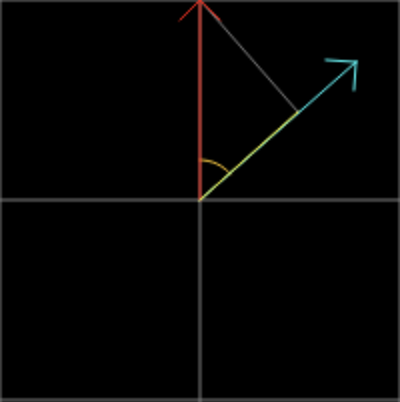
\includegraphics[width=120px]{images/dot-product.png}
    \caption{Dot product visualisation from \texttt{https://falstad.com/dotproduct}}
\end{figure}

Most following experiments were based the dot product between the start angle vector ($\mathbf{a}$, visualised in red) and the current angle vector ($\mathbf{b}$, visualised in blue). As a quick reminder, the dot product between two vectors $\mathbf{a}$ and $\mathbf{b}$ is defined by:

$$\mathbf{a}\cdot\mathbf{b}=\|\mathbf{a}\|\ \|\mathbf{b}\|\cos\theta$$

\noindent With some shuffling, the current angle ($\theta$, visualised in orange) can be found:

$$\theta = \arccos{( (\mathbf{a}\cdot\mathbf{b}) \div (\|\mathbf{a}\|\ \|\mathbf{b}\|) )}$$ 

To provide an offset from 0 to 1, the current angle must be divided by $2\pi$.
This was the initial attempt of translating the formula to code, it assumes the start angle parameter to be 0 for simplicity:

\begin{verbbox}[\small]
vec2 start_angle_vector = vec2(0.0, -V_CENTER.y);
float dot_prod = dot(start_angle_vector, pos - V_CENTER);
float current_angle = mod(
    acos(dot_prod / (V_CENTER.y * length(pos - V_CENTER))),
    2 * PI
);

float offset = current_angle / 2 * PI;
\end{verbbox}
\begin{figure}[H]
    $\vcenter{\hbox{
\includegraphics[width=100px]{images/shader-initial-attempt.png}}}$
    $\vcenter{\hbox{\theverbbox}}$\qquad
    \caption{Initial attempt}
\end{figure}

\noindent This had two main mistakes:

\begin{itemize}
    \item An overlooked bracketing mistake in the offset division: \texttt{current\_angle / (2 * PI)} should have been used instead of \texttt{current\_angle / 2 * PI}.
    
    \item When the current offset vector was on the left side, the current angle found from the dot product was the wrong one, the explement of that angle should have been chosen (e.g. the other angle that makes it add up to a full turn). See the figure below:
\begin{figure}[H]
    \centering
    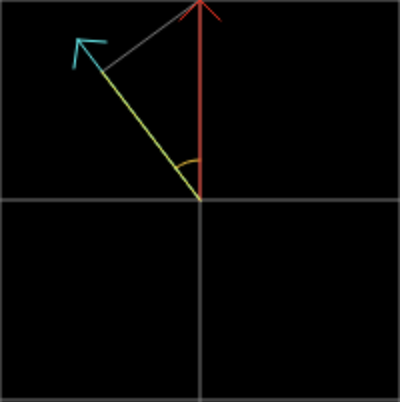
\includegraphics[width=120px]{images/dot-product-2.png}
\end{figure}
\end{itemize}

\noindent After fixing both of these problems, the result looked as expected:

\begin{verbbox}[\small]
vec2 current_dir = pos - V_CENTER;
vec2 start_angle_vector = vec2(0.0, -V_CENTER.y);
float dot_prod = dot(start_angle_vector, current_dir);
float current_angle = acos(dot_prod / (V_CENTER.y * length(current_dir)));
if (current_dir.x < 0) {
    current_angle = 2 * PI - current_angle;
}
current_angle = mod(current_angle, 2 * PI);

float offset = current_angle / (2 * PI);
\end{verbbox}
\begin{figure}[H]
    $\vcenter{\hbox{
\includegraphics[width=120px]{images/shader-final.png}}}$
    $\vcenter{\hbox{\theverbbox}}$\qquad
    \caption{Result after fixes}
\end{figure}


\noindent The previous code still assumed the start angle parameter to be 0, which needed to be fixed:

\begin{minted}{c}
vec2 current_dir = normalize(pos - V_CENTER);

float start_angle = PI / 2 - V_ANGLE;
vec2 start_vector = normalize(vec2(cos(start_angle), -sin(start_angle)));

float current_angle = acos(dot(start_vector, current_dir));
if (start_vector.x * current_dir.y - current_dir.x * start_vector.y < 0) {
    current_angle = 2 * PI - current_angle;
}
current_angle = mod(current_angle, 2 * PI);

float offset = current_angle / (2 * PI);
\end{minted}

 The formula found was ridiculously complicated, since it was thought out based on Cartesian coordinates. Markus Stange, a Gecko graphics engineer, suggested a simplified formula based on the previous attempt, presumably using polar coordinates:

\begin{minted}{c}
vec2 current_dir = pos - V_CENTER;
float current_angle = atan(current_dir.y, current_dir.x) + (PI / 2 - V_ANGLE);
float offset = mod(current_angle / (2 * PI), 1.0);
\end{minted}

This was the formula that was initially merged. The history of the formula can be found by browsing through the History tab of the Phabricator revision \cite{diff-webrender}.

With that formula, most cases rendered properly, except for gradients with first and last color stop offsets different than $0\%$ or $100\%$. An example taken from the polyfill website being:

\begin{verbatim}
conic-gradient(black 25%, white 0 50%, black 0 75%, white 0);
\end{verbatim}

This was fixed in a follow up commit \cite{diff-webrender-normalization} by normalising the offsets based on the first and last offsets, which led to the final version of the fragment shader:

\begin{minted}{c}
Fragment conic_gradient_brush_fs() {
    // [...]
    vec2 current_dir = pos - V_CENTER;
    float current_angle = atan(current_dir.y, current_dir.x) + (PI / 2.0 - V_ANGLE);
    float offset = mod(current_angle / (2.0 * PI), 1.0) - V_START_OFFSET;
    offset = offset / (V_END_OFFSET - V_START_OFFSET);

    vec4 color = sample_gradient(V_GRADIENT_ADDRESS,
                                 offset,
                                 V_GRADIENT_REPEAT);
    // [...]
    return Fragment(color);
}
\end{minted}


\subsection{Wrench}

Wrench is a debugging tool and testing framework for WebRender: it can replay recordings and execute YAML-based reference tests \cite{wrench-wiki}. Similar to other display item types, two methods needed to be added, along with related boilerplate code:

\begin{itemize}
    \item \texttt{handle\_conic\_gradient} in \texttt{yaml\_frame\_reader.rs}: handling the YAML \texttt{conic-gradient} item, by calling the WebRender API to push a conic gradient item to the display list.
    \item \texttt{conic\_gradient\_to\_yaml} in \texttt{yaml\_frame\_reader.rs}:  serialising conic gradient items to YAML, for WebRender recordings.
\end{itemize}

Here is an example YAML test for conic gradients:
\begin{minted}{yaml}
---
root:
  items:
    - type: conic-gradient
      bounds: 50 50 300 300
      center: 150 150
      angle: 0.0
      stops: [0.0, red, 1.0, yellow]
\end{minted}

This is equivalent to \texttt{conic-gradient(red, yellow)} on a 300×300 canvas.

The wrench test references are often PNG files, but they can also be another YAML file. References are linked together with the test using a metadata file called \texttt{reftest.list}.

Many reference tests were added for WebRender in a separate commit \cite{diff-webrender-tests}. Since the most relevant tests have been ported to Web Platform Tests, the testcases will be described in that section.

\section{Moz2D and Thebes}

In Firefox, there are many graphics backends, which means it is necessary to glue them together and abstract away the implementation details of each graphics backend. The part doing this is the Moz2D graphics API, which is an cross-platform interface onto the different backends. All current backends are interfaced by Moz2D, except for WebRender which uses its own API for interfacing. The code for Moz2D can be found in the \texttt{gfx/2d} directory.
Thebes is the API preceding Moz2D, but some parts are still in use today. \cite{moz2d}

Most of the code for Moz2D and Thebes is boilerplate code added along in the Skia implementation commit \cite{diff-skia}, but the main parts will be mentioned here:

\begin{itemize}
    \item The pattern class definition in \texttt{gfx/2d/2D.h}, describing a conic gradient pattern:
\begin{minted}{c}
class ConicGradientPattern : public Pattern {
 public:
  /// For constructor parameter description, see member data documentation.
  ConicGradientPattern(const Point& aCenter, Float aAngle, Float aStartOffset,
                       Float aEndOffset, GradientStops* aStops,
                       const Matrix& aMatrix = Matrix())
      : mCenter(aCenter),
        mAngle(aAngle),
        mStartOffset(aStartOffset),
        mEndOffset(aEndOffset),
        mStops(aStops),
        mMatrix(aMatrix) {}

  PatternType GetType() const override { return PatternType::CONIC_GRADIENT; }

  Point mCenter;       //!< Center of the gradient
  Float mAngle;        //!< Start angle of gradient
  Float mStartOffset;  // Offset of first stop
  Float mEndOffset;    // Offset of last stop
  RefPtr<GradientStops>
      mStops;      /**< GradientStops object for this gradient, this
                        should match the backend type of the draw target
                        this pattern will be used with. */
  Matrix mMatrix;  //!< A matrix that transforms the pattern into user space
};
\end{minted}
    \item The corresponding pattern type in \texttt{gfx/2d/Types.h}:
\begin{minted}{diff}
 enum class PatternType : int8_t {
   COLOR,
   SURFACE,
   LINEAR_GRADIENT,
   RADIAL_GRADIENT,
+  CONIC_GRADIENT
 };
\end{minted}
    \item The \texttt{gfxPattern} constructor for conic gradients in \texttt{gfx/thebes/gfxPattern.cpp}, called by the web painting code:
\begin{minted}{c}
gfxPattern::gfxPattern(gfxFloat cx, gfxFloat cy, gfxFloat angle,
                       gfxFloat startOffset, gfxFloat endOffset)
    : mExtend(ExtendMode::CLAMP) {
  mGfxPattern.InitConicGradientPattern(Point(cx, cy), angle, startOffset,
                                       endOffset, nullptr);
}
\end{minted}
    \item Code abstracting different backends represented as ``draw targets''. The implementation for the Skia draw target will be described in the next section.
\end{itemize}

\section{Skia}

In Firefox, Skia is the graphics backend used by default on Linux, Android, macOS and a very small subset of Windows devices \cite{direct2d-blocklist}. It is a graphics library maintained by Google, other popular projects using it include Google Chrome, Chrome OS and Android \cite{skia}.

Implementing conic gradients for Skia \cite{diff-skia} mainly consisted of adding a case for conic gradient patterns in the \texttt{SetPaintPattern} method for \texttt{DrawTargetSkia.cpp}:

\begin{minted}{diff}
 static void SetPaintPattern(SkPaint& aPaint, const Pattern& aPattern,
                             Float aAlpha = 1.0,
                             const SkMatrix* aMatrix = nullptr,
                             const Rect* aBounds = nullptr) {
   switch (aPattern.GetType()) {
     // [...]
+    case PatternType::CONIC_GRADIENT: {
+      const ConicGradientPattern& pat =
+          static_cast<const ConicGradientPattern&>(aPattern);
+      GradientStopsSkia* stops =
+          static_cast<GradientStopsSkia*>(pat.mStops.get());
+      if (!stops || stops->mCount < 2 || !pat.mCenter.IsFinite() ||
+          !IsFinite(pat.mAngle)) {
+        aPaint.setColor(SK_ColorTRANSPARENT);
+      } else {
+        SkMatrix mat;
+        GfxMatrixToSkiaMatrix(pat.mMatrix, mat);
+        if (aMatrix) {
+          mat.postConcat(*aMatrix);
+        }
+
+        SkScalar cx = SkFloatToScalar(pat.mCenter.x);
+        SkScalar cy = SkFloatToScalar(pat.mCenter.y);
+
+        // Skia's sweep gradient angles are relative to the x-axis, not the
+        // y-axis.
+        Float angle = (pat.mAngle * 180.0 / M_PI) - 90.0;
+        if (angle != 0.0) {
+          mat.preRotate(angle, cx, cy);
+        }
+
+        SkTileMode mode = ExtendModeToTileMode(stops->mExtendMode, Axis::BOTH);
+        sk_sp<SkShader> shader = SkGradientShader::MakeSweep(
+            cx, cy, &stops->mColors.front(), &stops->mPositions.front(),
+            stops->mCount, mode, 360 * pat.mStartOffset, 360 * pat.mEndOffset,
+            0, &mat);
+
+        if (shader) {
+          aPaint.setShader(shader);
+        } else {
+          aPaint.setColor(SK_ColorTRANSPARENT);
+        }
+      }
+      break;
+    }
     // [...]
   }
 }
\end{minted}

\noindent Like for other gradients:
\begin{itemize}
    \item the parameters are passed in from the Moz2D API
    \item the box is painted transparent in case of invalid parameters or failure
    \item transformation matrices are converted and applied at this point (for CSS transforms)
\end{itemize}

As for the shader, \mintinline{cpp}{SkGradientShader::MakeSweep} was the right method according to the Skia documentation \cite{skia-shader-docs}. The initial Skia implementation used the following parameters:

\begin{minted}{cpp}
sk_sp<SkShader> shader = SkGradientShader::MakeSweep(
    cx, cy, &stops->mColors.front(), &stops->mPositions.front(),
    stops->mCount, 0, &mat);
\end{minted}

\noindent Unfortunately, while this worked well for many cases, two cases from the polyfill website were broken:

\begin{itemize}
    \item \texttt{conic-gradient(red -50\%, gold 110\%)} rendered the same as \texttt{conic-gradient(red 0\%, gold 100\%)}.
\begin{figure}[H]
  \begin{subfigure}[b]{0.5\textwidth}
    \centering
    
\includegraphics[width=0.7\textwidth]{images/skia-broken-ref.png}
    \caption{Expected}
  \end{subfigure}
  \hfill
  \begin{subfigure}[b]{0.5\textwidth}
    \centering
    
\includegraphics[width=0.7\textwidth]{images/skia-broken.png}
    \caption{Broken}
  \end{subfigure}
\end{figure}
    \item \texttt{repeating-conic-gradient} rendered the same as its \texttt{conic-gradient} counterpart.
\begin{figure}[H]
  \begin{subfigure}[b]{0.5\textwidth}
    \centering
    
\includegraphics[width=0.7\textwidth]{images/not-so-repeating-gradient-ref.png}
    \caption{Expected}
  \end{subfigure}
  \hfill
  \begin{subfigure}[b]{0.5\textwidth}
    \centering
    
\includegraphics[width=0.7\textwidth]{images/not-so-repeating-gradient.png}
    \caption{Broken}
  \end{subfigure}
\end{figure}
\end{itemize}

To fix this issue, Blink's implementation of conic gradients was checked to see how Skia was used. Blink first calls \mintinline{cpp}{PaintShader::MakeSweepGradient} \cite{skia-chromium-conic}, which indirectly calls \mintinline{cpp}{SkGradientShader::MakeSweep} \cite{skia-chromium-conic-2} \cite{skia-chromium-conic-3}. However, it uses a 10-argument version that was not found on the Skia shader documentation \cite{skia-shader-docs}, as opposed to the 7-argument version used in my initial implementation.

The extra arguments were:
\begin{itemize}
    \item start offset: the position of the first color stop
    \item end offset: the position of the last color stop
    \item extend mode: this determines how the image is extended outside the bounds of the image. The same extend mode other gradient types used was chosen.
\end{itemize}

Similarly to WebRender, the start offset and the end offset were needed for Skia to properly render the shader. They needed to be converted from percentages to degrees, by multiplying the value by 360.

\begin{minted}{diff}
+        SkTileMode mode = ExtendModeToTileMode(stops->mExtendMode, Axis::BOTH);
         sk_sp<SkShader> shader = SkGradientShader::MakeSweep(
             cx, cy, &stops->mColors.front(), &stops->mPositions.front(),
-            stops->mCount, 0, &mat);
+            stops->mCount, mode, 360 * pat.mStartOffset, 360 * pat.mEndOffset,
+            0, &mat);
\end{minted}

\section{Web Platform Tests}

Web Platform Tests (abbreviated as WPT) is a cross-browser test suite than runs on all major browser engines (Blink/Chromium, WebKit and Gecko). It contains tests contributed from Mozilla, Google, Apple, but also from independent contributors. The main aim of web platform tests to ensure that implementations by one browser engine are compatible with other browser engines and prevent web compatibility issues \cite{wpt-readme}. Tests can be contributed by sending a pull request to the upstream Github repository, but can also be contributed directly in the Chromium or Firefox source code, in which case they will be synced back to the upstream project by a bot.

In Firefox, web platform tests are setup in three parts:
\begin{itemize}
    \item the metadata, consisting of INI files with preferences that need to be enabled and the tests that are expected to fail. The metadata is specific to the Firefox source code.
    \item the tests themselves, written in web technologies, which are synced with the Github repository
    \item the tooling, which takes care of synchronising and running the tests. It is not directly relevant to this project.
\end{itemize}

Tests automatically fail when the metadata is incorrect, e.g. when a test is marked as expected to fail, but actually passes, or vice-versa. They can be ran using the \texttt{./mach wpt} command in Firefox.

\subsection{Updating the metadata}
For conic gradients, three web platform tests were already written by external people:
\begin{itemize}
    \item a \texttt{background-image} parsing test (\texttt{css/css-images/gradient/color-stops-parsing.html}), which tested that gradient functions with different parameters were correctly parsed in the \texttt{background-image} CSS property. This test was contributed by Florin Malita, a Google engineer. \cite{wpt-color-stop-parsing}
    \item a \texttt{border-image-source} serialisation test (\texttt{border-image-source-computed.sub.html}), testing the correctness of the \texttt{getComputedStyle()} serialisation for the \texttt{border-image-source} CSS property, which includes gradient values. This test was contributed by Eric Willigers, a Chromium contributor. \cite{wpt-border-image-source-computed}
    \item a rendering test (\texttt{css/css-images/multiple-position-color-stop-conic.html}), which tested that conic gradient with 2 hard color stops were rendered correctly. It was contributed by Fredrik Söderquist, at the time working at Opera. \cite{wpt-multiple-position-color-stop-conic}
\end{itemize}
The metadata marked those three tests as failing. The implementation done for this project made those tests pass when ran with the conic gradient feature flag enabled.
The metadata was updated to enable the feature flag for those tests instead of marking them as failing \cite{wpt-expectations}. For instance:
\begin{minted}{ini}
[border-image-source-computed.sub.html]
  [Property border-image-source value 'conic-gradient(from 90deg at 80% 90%, lime, black)']
    expected: FAIL
\end{minted}
was updated to:
\begin{minted}{ini}
[border-image-source-computed.sub.html]
  prefs: [layout.css.conic-gradient.enabled:true]
\end{minted}


Early on during the implementation, the rendering test failed for WebRender only, due to color stop normalisation issues, this was fixed as described in the WebRender section.

Having tests contributed by external contributors start passing confirms the correctness of the implementation. However, one rendering test was not enough to test different edge cases of conic gradients, so more test cases were added.

\subsection{Adding new tests}

There was only one pre-existing rendering web platform test for conic gradients, compared to 14 rendering tests for linear gradients and 7 for radial gradients. It is reasonable that radial or conic gradients have less tests than linear gradients, since some linear gradient tests actually test shared code between all three gradient types. Tests were written and merged to test different edge cases of conic gradients. Most were based on wrench tests written earlier on in the project for WebRender, but used HTML and CSS instead of YAML files.

Here is an example from the \texttt{normalization-conic.html} test:

\begin{minted}{html}
<!doctype html>
<meta charset="utf-8">
<title>Conic gradient stop normalization</title>
<link rel="help" href="https://drafts.csswg.org/css-images-4/#conic-gradients">
<meta name="assert" content="Rendering of conic-gradient with normalized color stops">
<link rel="match" href="reference/100x100-blue.html">
<style>
  #gradient {
    width: 100px;
    height: 100px;
    background-image: conic-gradient(green -50%, blue -50%);
  }
</style>
<div id="gradient"></div>
\end{minted}


\noindent A web platform test is simply an HTML file:
\begin{itemize}
    \item The HTML doctype and the charset meta tag are not necessary for conic gradients, but it is good practice to include them in any web page.
    \item The help link tag links to the specification
    \item The assert meta tag describes what is being tested
    \item The match link tag links to the matching reference file, in this case, rendering a blue square:
\begin{minted}{html}
<!doctype html>
<div style="width: 100px;height: 100px;background-color: blue;"></div>
\end{minted}
\end{itemize}

\noindent The complete commit adding the tests can be found on Phabricator \cite{wpt-new-tests} and the tests can be categorised as such:
\begin{itemize}
    \item Tests for conic gradients in a basic configuration.
\begin{verbatim}
testing/web-platform/tests/css/css-images/conic-gradient-angle-negative.html
testing/web-platform/tests/css/css-images/conic-gradient-angle.html
testing/web-platform/tests/css/css-images/conic-gradient-center.html
testing/web-platform/tests/css/css-images/multiple-position-color-stop-conic-2.html
testing/web-platform/tests/css/css-images/repeating-conic-gradient.html
testing/web-platform/tests/css/css-images/tiled-conic-gradients.html
\end{verbatim}
    \item Tests for gradients with color stops outside the range of 0 to 100\%, since both the Skia and WebRender had related bugs early on the implementation as mentioned previously.
\begin{verbatim}
testing/web-platform/tests/css/css-images/normalization-linear-2.html
testing/web-platform/tests/css/css-images/normalization-linear.html
testing/web-platform/tests/css/css-images/normalization-radial-2.html
testing/web-platform/tests/css/css-images/normalization-radial.html
testing/web-platform/tests/css/css-images/normalization-conic-2.html
testing/web-platform/tests/css/css-images/normalization-conic.html
testing/web-platform/tests/css/css-images/out-of-range-color-stop-conic.html
\end{verbatim}
    \item Tests for the degenerate case, where a repeating gradient has two stops at the same position (e.g. \mintinline{css}{repeating-conic-gradient(orange 50%, blue 50%)}), in which case the element should be completely filled with the second color (blue).
\begin{verbatim}
testing/web-platform/tests/css/css-images/normalization-linear-degenerate.html
testing/web-platform/tests/css/css-images/normalization-radial-degenerate.html
testing/web-platform/tests/css/css-images/normalization-conic-degenerate.html
\end{verbatim}
\end{itemize}

\subsection{Interoperability of tests}

When adding new web platform tests, it is important to check whether the references for the tests are correct and interoperable with other web browsers.

Having the tests reviewed by an experienced Gecko engineer and merged \cite{wpt-new-tests} is usually enough to check the correctness, but it only guarantees that the tests pass in Firefox. It is possible that mistakes are overlooked, which is why it is worth checking how the test results for other browsers.

To do this, there is a website called wpt.fyi, which is a dashboard showing results from web platform test runs for major browsers. It is worth noting that wpt.fyi does not take in account the test metadata from different browsers, meaning that feature flags will not be turned on, which causes Firefox results to be marked as failed.

The run tested the latest alpha versions of each browser and can be found at \cite{wpt-fyi}. The results can be found in the screenshot below:

\begin{figure}[H]
    \centering
    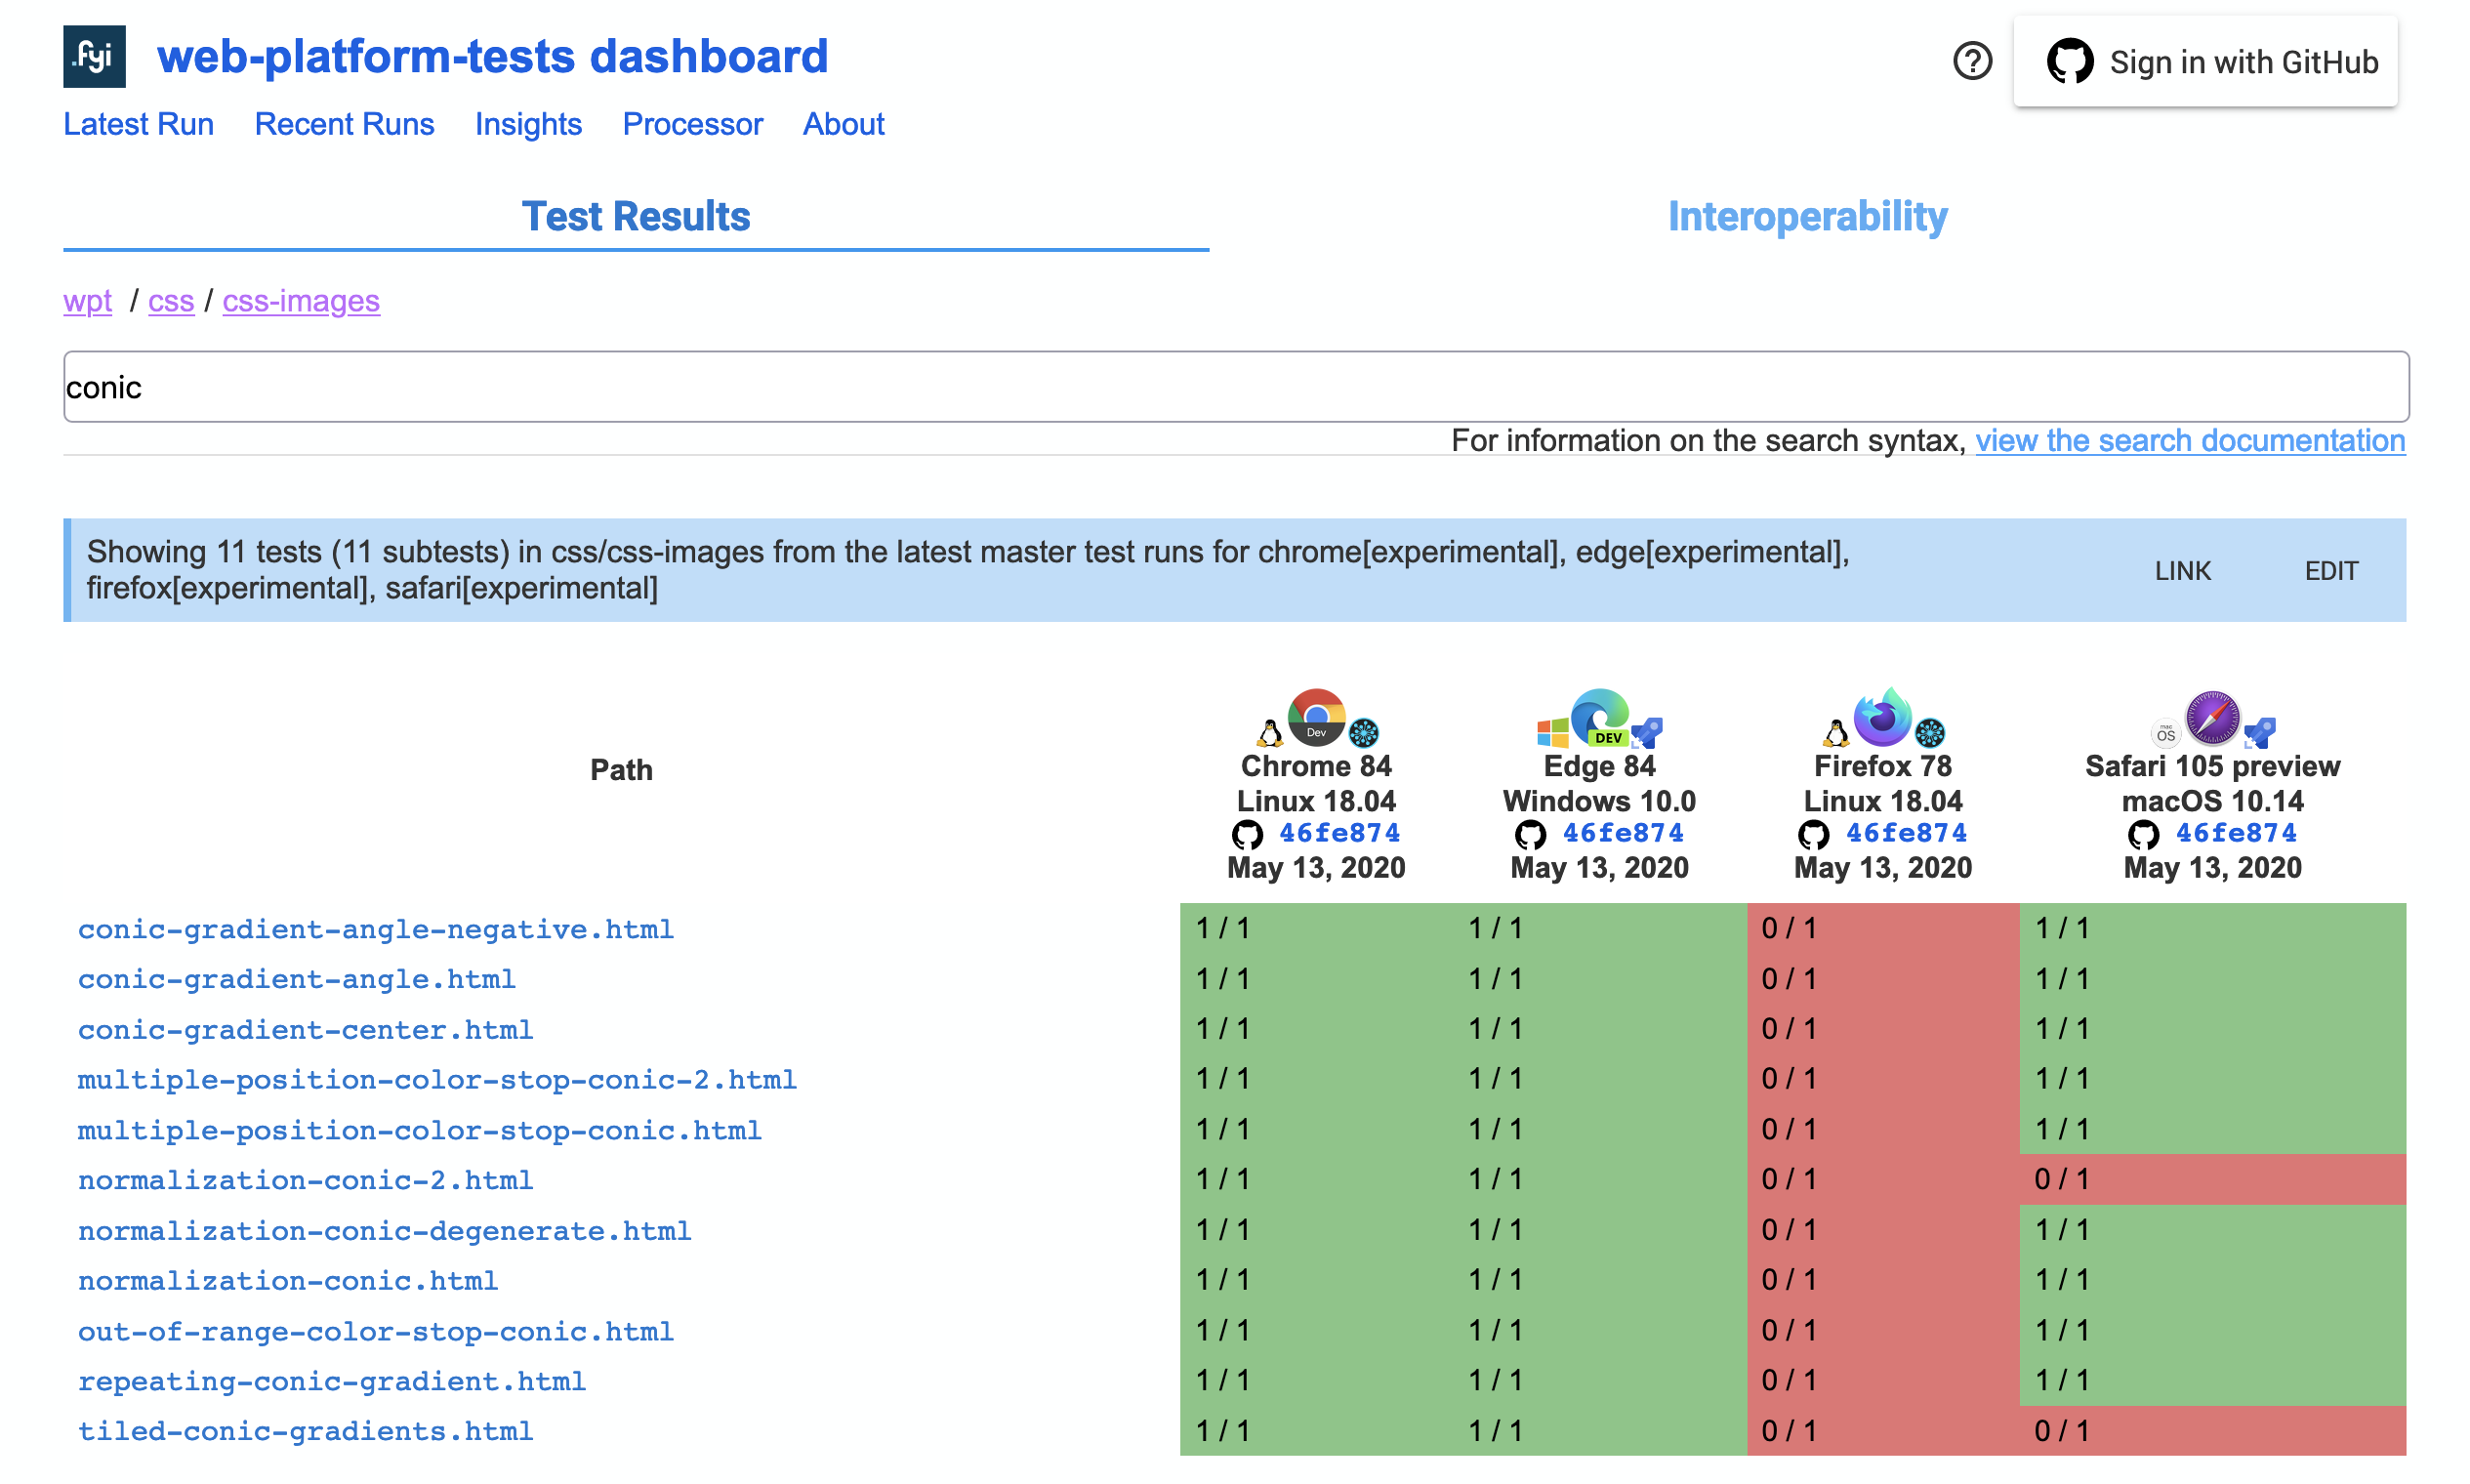
\includegraphics[width=\textwidth]{images/wpt-fyi.png}
    \caption{wpt.fyi results for conic gradient related tests}
\end{figure}

As seen in the screenshot above, all conic gradient tests are passing in Chromium and most of them pass in Safari (which uses WebKit).

It turns out the \texttt{normalization-conic-2.html} test (written part of this project) reveals a bug in WebKit's implementation, which is why the test was failing.
This test uses an element filled with \texttt{conic-gradient(blue 150\%, red 150\%)} which should render a blue square. However, Safari renders a transparent square:

\begin{figure}[H]
  \begin{subfigure}[t]{0.5\textwidth}
    \centering
    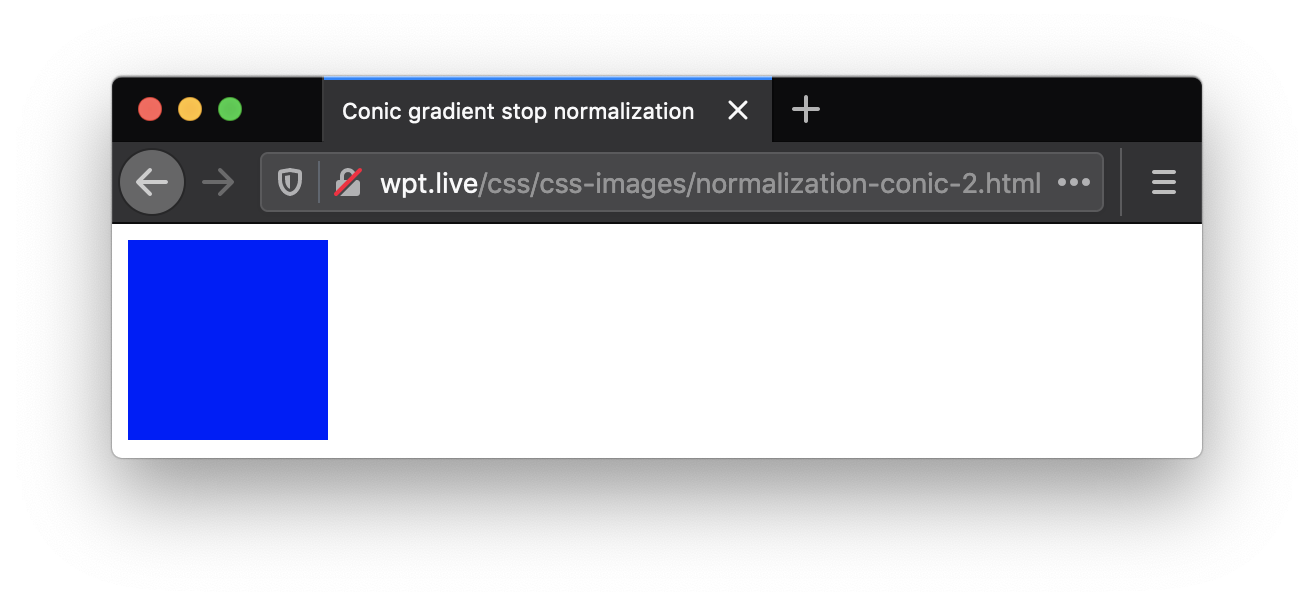
\includegraphics[width=0.8\textwidth]{images/webkit-bug-ref.png}
    \caption{Expected (Chromium and Firefox)}
  \end{subfigure}
  \hfill
  \begin{subfigure}[t]{0.5\textwidth}
    \centering
    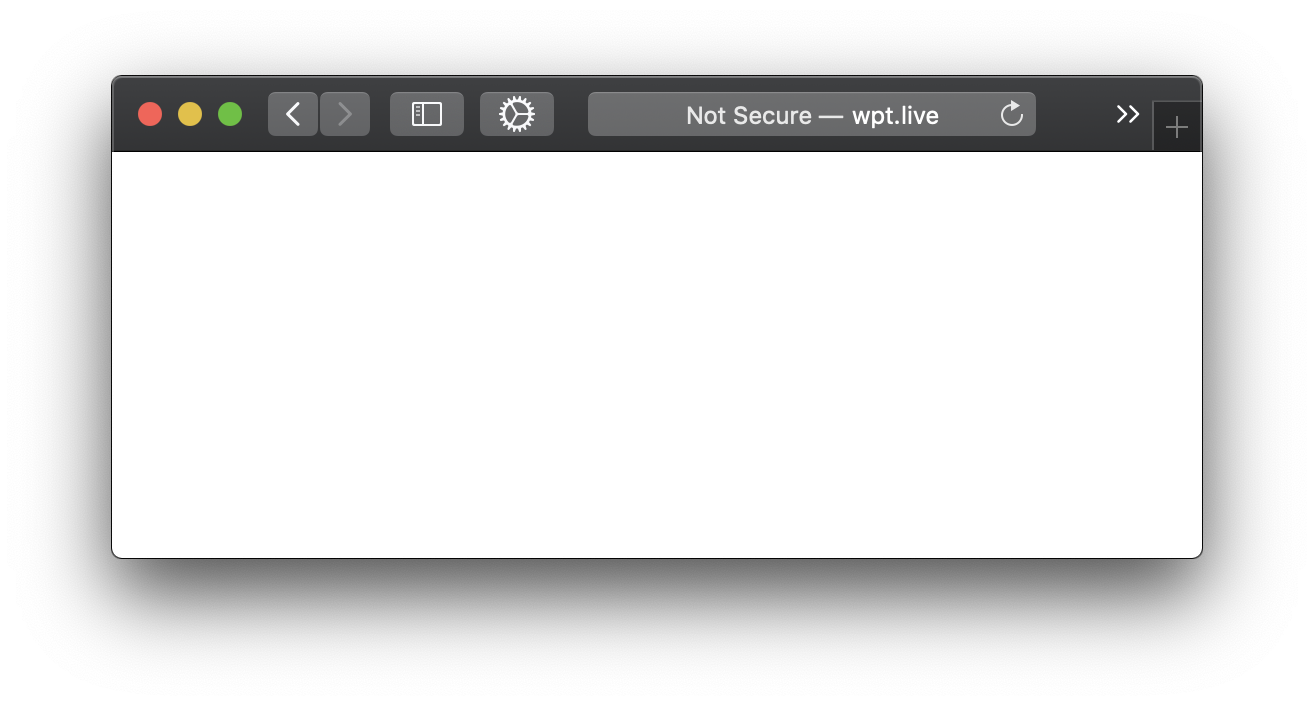
\includegraphics[width=0.8\textwidth]{images/webkit-bug.png}
    \caption{Broken (Safari)}
  \end{subfigure}
\end{figure}

The other failing test, \texttt{tiled-conic-gradients.html}, is a small rendering glitch, that is not seen when ran live on Safari, so it is safe to assume that this may be related to the hardware used by wpt.fyi: 

\begin{figure}[H]
    \centering
    
\includegraphics[width=200px]{images/webkit-bug-ok.png}
    \caption{Graphical glitch on tiled-conic-gradients.html}
\end{figure}

\section{Developer Tools support}

Like other browsers, Firefox has developer tools for web developers to debug their webpages.
The developer tool requiring extra work for this project is the inspector tool (also named the elements tool in other web browsers). This tool allows inspecting the structure of the webpage and displays a sidebar which shows the CSS styles for the selected element.


\begin{figure}[H]
    \centering
    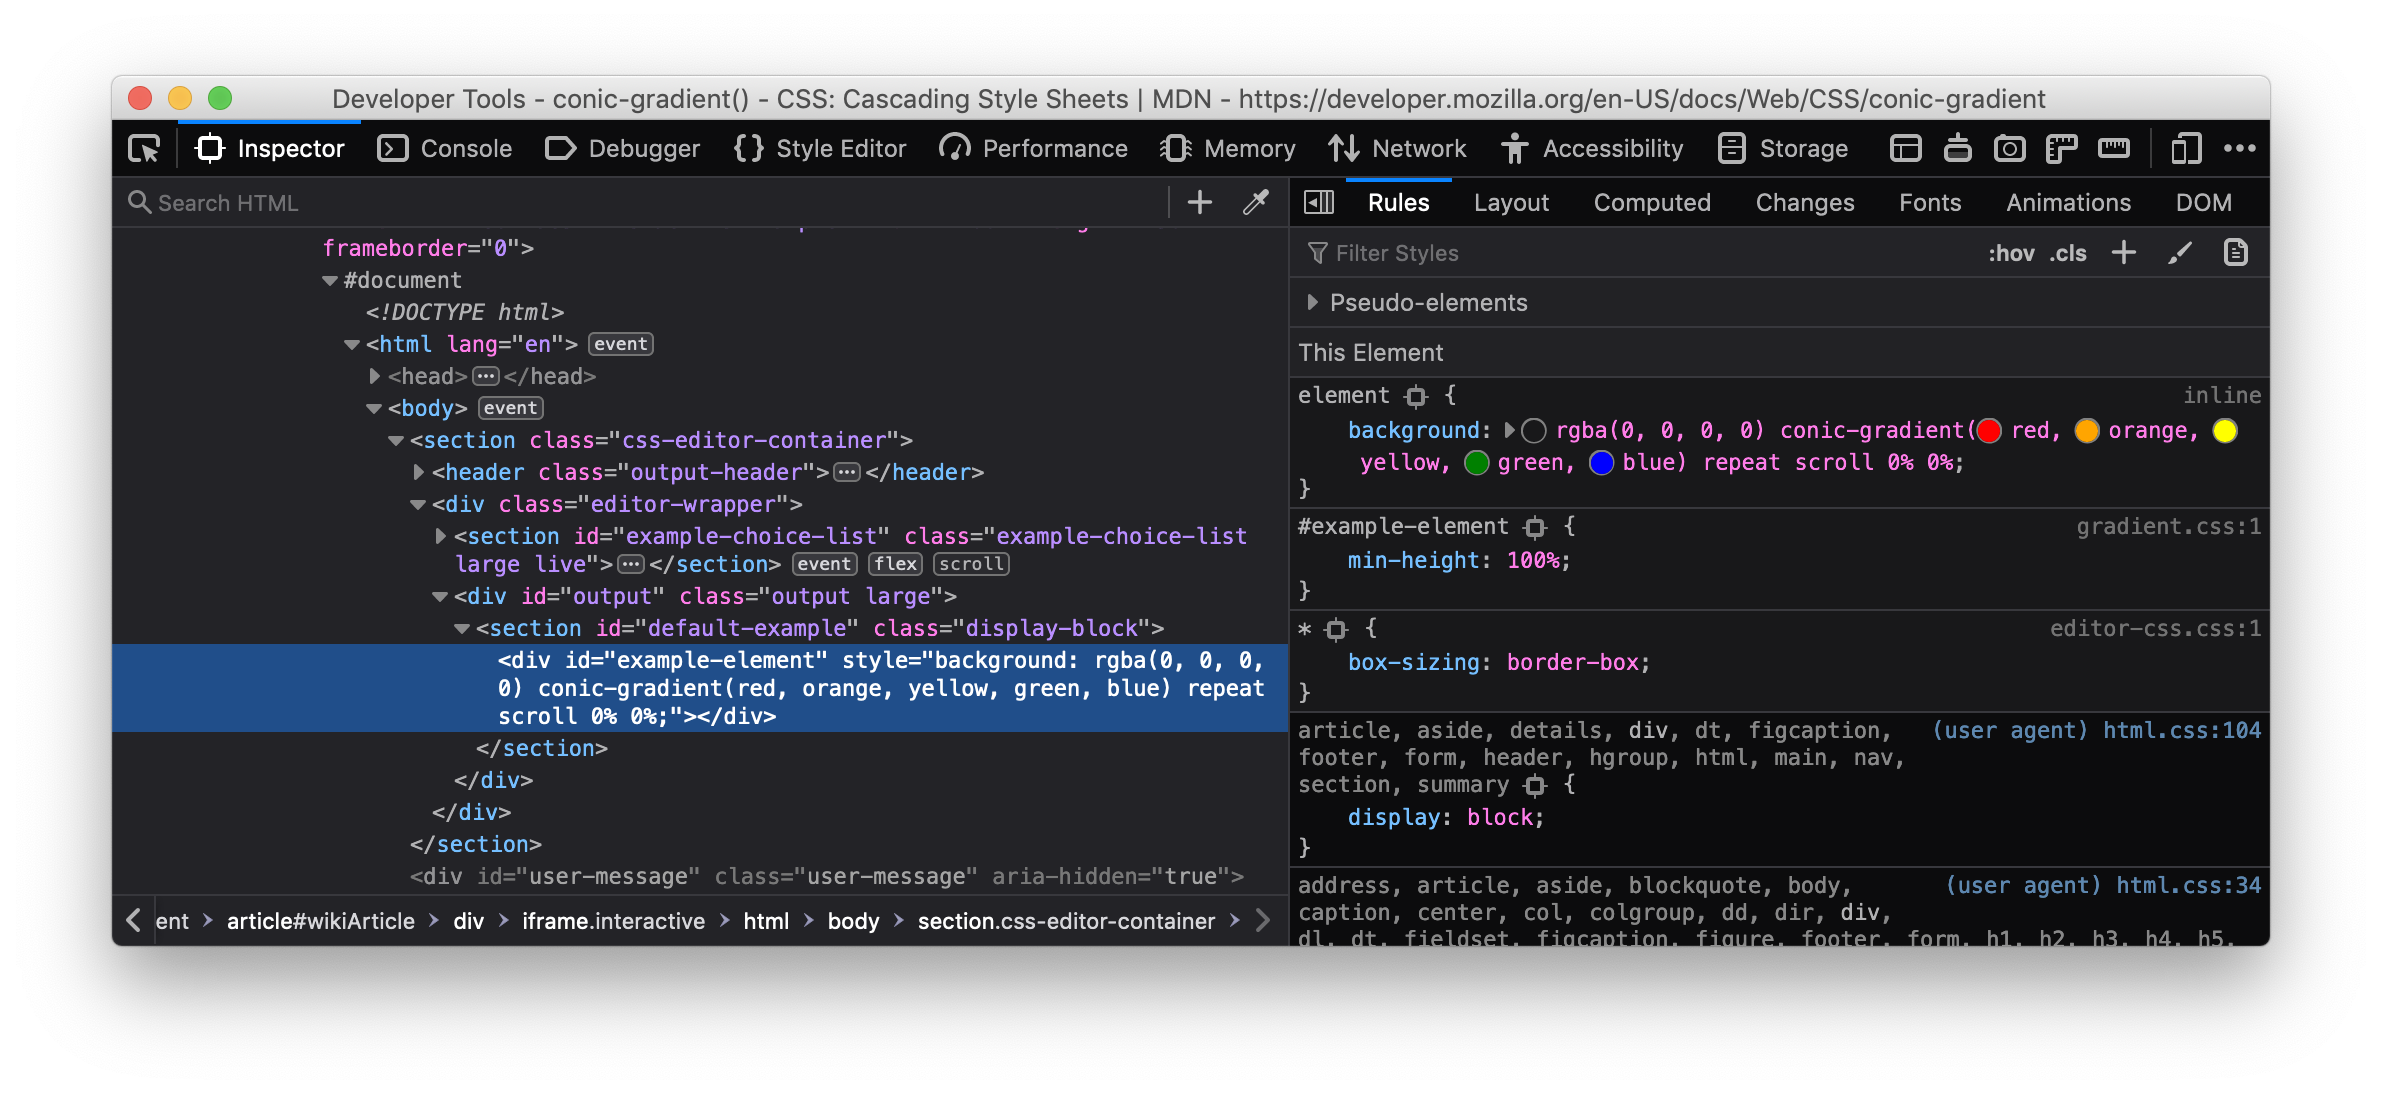
\includegraphics[width=\textwidth]{images/inspector.png}
    \caption{Firefox Inspector tool}
    \label{fig:inspector}
\end{figure}

The inspector works with and understands the newly added CSS feature without any extra effort.
However, some bits of the inspector need extra work to provide an optimal experience for developers.

\subsection{Auto-completion}

To make authoring faster, tools usually suggest keywords inside a popup, so the user can simply
type a part of a keyword and select it to get the whole keyword. The inspector is no exception:

\begin{figure}[H]
    \centering
    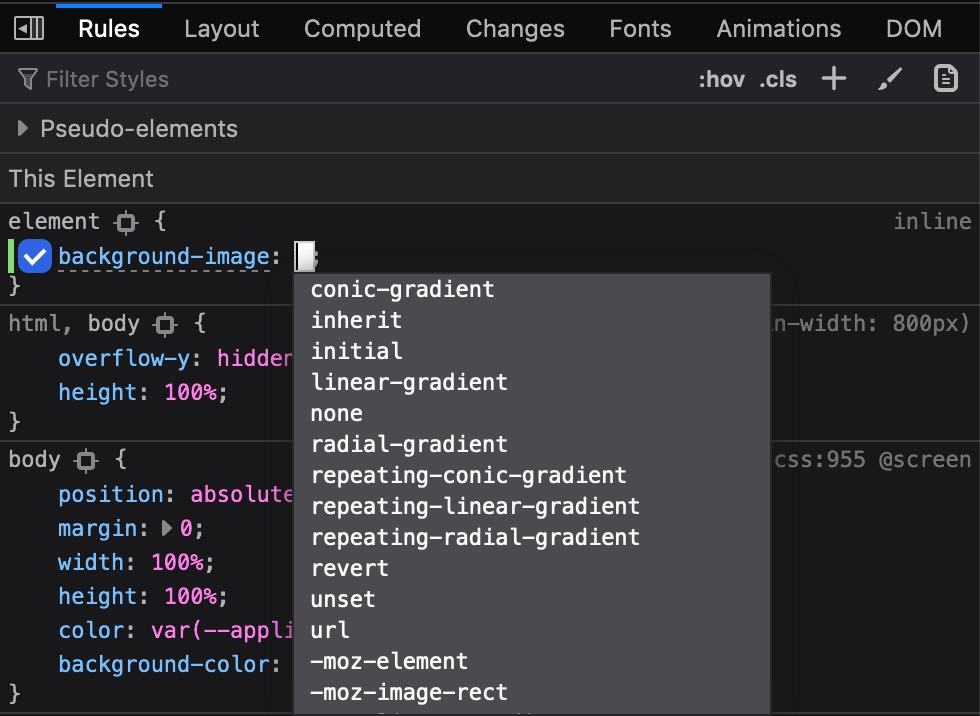
\includegraphics[width=0.75\textwidth]{images/inspector-autocomplete.png}
    \caption{Auto-completion in the Rules view}
    \label{fig:inspector_autocomplete}
\end{figure}

To add conic gradients to the autocompletion list, the existing \texttt{collect\_completion\_keywords} function in the style system was extended:
    
\begin{minted}{diff}
 fn collect_completion_keywords(f: KeywordsCollectFn) {
     f(&[
         // [...]
     ]);
 
+    if static_prefs::pref!("layout.css.conic-gradient.enabled") {
+        f(&[
+            "conic-gradient",
+            "repeating-conic-gradient",
+        ]);
+    }
 }
\end{minted}

\subsection{Color and angle swatches}

For convenience and to make the developer tool require less technical knowledge to use, Firefox has added swatches for colors and angles. Clicking the color swatch brings up a color picker, and clicking it while holding the ``Shift'' key switches between color formats. As for the angle swatch, clicking it while holding ``Shift'' switches between different angle units. 

\begin{figure}[H]
    \centering
    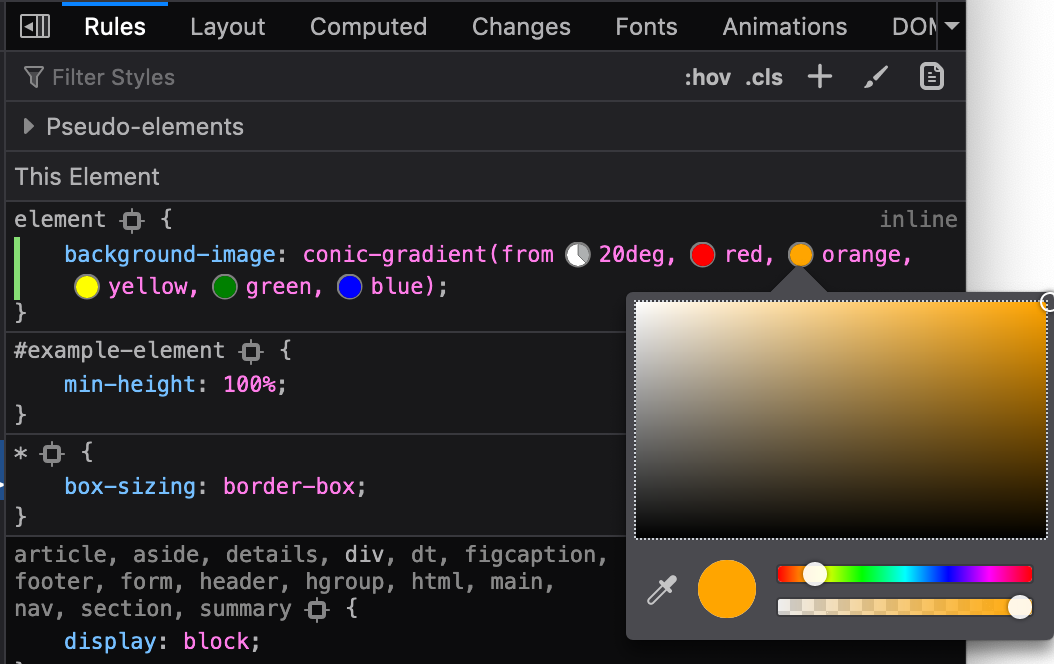
\includegraphics[width=0.75\textwidth]{images/inspector-swatches.png}
    \caption{Swatches in the Rules view}
    \label{fig:inspector_swatch}
\end{figure}

Those are already shown for other CSS functions using angles or colors, but were not initially
shown for conic gradients. To fix this, cases were added to the developer tools output
parser (in \texttt{devtools/client/shared/output-parser.js}):

\begin{minted}{javascript}
const CONIC_GRADIENT_ENABLED = Services.prefs.getBoolPref(
  "layout.css.conic-gradient.enabled"
);

// Functions that accept an angle argument.
const ANGLE_TAKING_FUNCTIONS = [
  // [...]
  ...(CONIC_GRADIENT_ENABLED
    ? ["conic-gradient", "repeating-conic-gradient"]
    : []),
  // [...]
];

// Functions that accept a color argument.
const COLOR_TAKING_FUNCTIONS = [
  // [...]
  ...(CONIC_GRADIENT_ENABLED
    ? ["conic-gradient", "repeating-conic-gradient"]
    : []),
  "drop-shadow",
];
\end{minted}


\section{HTML canvas API}

The HTML \texttt{<canvas>} element enables drawing graphics and animations using the canvas JavaScript API (known as \texttt{CanvasRenderingContext2D}). It may be used in cases where rendering multiple HTML elements styled with CSS may be inefficient, for instance games where high performance may be essential.

There are existing \texttt{createLinearGradient} and \texttt{createRadialGradient} functions that are in the HTML specification, but there is not currently any \texttt{createConicGradient} 
function. I have filed an issue on the specification Github repository and there is some early work-in-progress specification work being done in collaboration with the Google Chrome team \cite{ntim-issue-conic-gradient}. The current function definition decided on is:

\begin{minted}{c}
interface mixin CanvasFillStrokeStyles {
  ...
  CanvasGradient createConicGradient(double angle, double cx, double cy);
};
\end{minted}

The \texttt{angle} parameter is analogous to the one in the CSS function, while the \texttt{cx} and \texttt{cy} parameters represent the position/center parameter from the CSS function.

Here is an example usage from the work-in-progress proposal \cite{fserb-conic-gradient}:
\begin{minted}{javascript}
const canvas = document.createElement("canvas");
const ctx = canvas.getContext("2d");

const grad = ctx.createConicGradient(0, 100, 100);

grad.addColorStop(0, "red");
grad.addColorStop(0.25, "orange");
grad.addColorStop(0.5, "yellow");
grad.addColorStop(0.75, "green");
grad.addColorStop(1, "blue");

ctx.fillStyle = grad;
ctx.fillRect(0, 0, 200, 200);
document.body.append(canvas);
\end{minted}

For this project, an implementation has been made in the Firefox rendering engine \cite{diff-canvas}. However, it has not been merged and tests have not yet been written, since it is awaiting for the final specification. The code for the canvas API is located in the \texttt{dom/canvas/} directory. The function declaration was added to the \texttt{WebIDL} file, which defines the JavaScript methods exposed to the web. The rest of the implementation was analogous to the existing radial or linear gradient counterparts, adjusted for the different conic gradient parameters and re-used the CSS \texttt{conic-gradient} function graphics code.

\section{Future work}
\subsection{Direct2D}

One remaining part of this project is the implementation for the Direct2D backend. This is the only remaining bit of work needed to enable conic gradients by default for all users. Direct2D is used on Windows when WebRender is not supported by the underlying hardware. In rare cases where Direct2D is not supported, Skia is used as a fallback \cite{direct2d-blocklist}. Skia could technically be used on all Windows machines, as the library supports it, but Direct2D was chosen by the graphics team since it has a better performance due to being designed specifically for Windows by Microsoft.

For Direct2D, an untested work in progress commit developed on macOS was submitted \cite{diff-d2d} and will be described here.
Conic gradients on Direct2D can be done using the mesh gradient library methods, however those methods are only available on Windows 10 and above \cite{mesh-gradients-win10}, so they cannot be used in Firefox which has to support Windows 7 and 8. However, a solution that works on all versions of Windows would be creating a custom effect (similar to shaders) and rendering it. The work in progress commit uses this approach, based on the WebRender shader and the existing radial gradient code, but it cannot be tried out and finished without a Windows development environment.

\subsection{Cairo}

Implementing conic gradients for printing was deemed low priority by the Firefox Layout team because the \texttt{background-image} CSS property, which is the main use-case for conic gradients, is disabled by default when printing web pages for readability and can only be enabled with an internal preference \cite{internal-pref-printing}. Given this fact, implementing printing support is not essential to enable conic gradient by default.

However, if this were to be done, a possible approach would be to use Skia to render the conic gradient into a surface and pass that surface to DrawTargetCairo for printing. An alternative approach would be using the Cairo APIs to draw the gradient, it is more complex
but provides greater rendering performance, which does not matter much with printing.

% This chapter is intended to describe what you did: the goal is to explain
% the main activity or activities, of any type, which constituted your work 
% during the project.  The content is highly topic-specific, but for many 
% projects it will make sense to split the chapter into two sections: one 
% will discuss the design of something (e.g., some hardware or software, or 
% an algorithm, or experiment), including any rationale or decisions made, 
% and the other will discuss how this design was realised via some form of 
% implementation.  

% This is, of course, far from ideal for {\em many} project topics.  Some
% situations which clearly require a different approach include:

% \begin{itemize}
% \item In a project where asymptotic analysis of some algorithm is the goal,
%       there is no real ``design and implementation'' in a traditional sense
%       even though the activity of analysis is clearly within the remit of
%       this chapter.
% \item In a project where analysis of some results is as major, or a more
%       major goal than the implementation that produced them, it might be
%       sensible to merge this chapter with the next one: the main activity 
%       is such that discussion of the results cannot be viewed separately.
% \end{itemize}

% \noindent
% Note that it is common to include evidence of ``best practice'' project 
% management (e.g., use of version control, choice of programming language 
% and so on).  Rather than simply a rote list, make sure any such content 
% is useful and/or informative in some way: for example, if there was a 
% decision to be made then explain the trade-offs and implications 
% involved.


% \section{Example Section}

% This is an example section; 
% the following content is auto-generated dummy text.
% \lipsum

% \subsection{Example Sub-section}

% \begin{figure}[t]
% \centering
% foo
% \caption{This is an example figure.}
% \label{fig}
% \end{figure}

% \begin{table}[t]
% \centering
% \begin{tabular}{|cc|c|}
% \hline
% foo      & bar      & baz      \\
% \hline
% $0     $ & $0     $ & $0     $ \\
% $1     $ & $1     $ & $1     $ \\
% $\vdots$ & $\vdots$ & $\vdots$ \\
% $9     $ & $9     $ & $9     $ \\
% \hline
% \end{tabular}
% \caption{This is an example table.}
% \label{tab}
% \end{table}

% \begin{algorithm}[t]
% \For{$i=0$ {\bf upto} $n$}{
%   $t_i \leftarrow 0$\;
% }
% \caption{This is an example algorithm.}
% \label{alg}
% \end{algorithm}

% \begin{lstlisting}[float={t},caption={This is an example listing.},label={lst},language=C]
% for( i = 0; i < n; i++ ) {
%   t[ i ] = 0;
% }
% \end{lstlisting}

% This is an example sub-section;
% the following content is auto-generated dummy text.
% Notice the examples in Figure~\ref{fig}, Table~\ref{tab}, Algorithm~\ref{alg}
% and Listing~\ref{lst}.
% \lipsum

% \subsubsection{Example Sub-sub-section}

% This is an example sub-sub-section;
% the following content is auto-generated dummy text.
% \lipsum

% \paragraph{Example paragraph.}

% This is an example paragraph; note the trailing full-stop in the title,
% which is intended to ensure it does not run into the text.

% -----------------------------------------------------------------------------

% \chapter{Critical Evaluation}
% \label{chap:evaluation}

% {\bf A topic-specific chapter, of roughly $15$ pages} 
% \vspace{1cm} 

% \noindent
% This chapter is intended to evaluate what you did.  The content is highly 
% topic-specific, but for many projects will have flavours of the following:

% \begin{enumerate}
% \item functional  testing, including analysis and explanation of failure 
%       cases,
% \item behavioural testing, often including analysis of any results that 
%       draw some form of conclusion wrt. the aims and objectives,
%       and
% \item evaluation of options and decisions within the project, and/or a
%       comparison with alternatives.
% \end{enumerate}

% \noindent
% This chapter often acts to differentiate project quality: even if the work
% completed is of a high technical quality, critical yet objective evaluation 
% and comparison of the outcomes is crucial.  In essence, the reader wants to
% learn something, so the worst examples amount to simple statements of fact 
% (e.g., ``graph X shows the result is Y''); the best examples are analytical 
% and exploratory (e.g., ``graph X shows the result is Y, which means Z; this 
% contradicts [1], which may be because I use a different assumption'').  As 




% such, both positive {\em and} negative outcomes are valid {\em if} presented 
% in a suitable manner.

% -----------------------------------------------------------------------------

\chapter{Conclusion}
\label{chap:conclusion}

% {\bf A compulsory chapter,     of roughly $5$ pages} 
\vspace{1cm} 

% \noindent
% The concluding chapter of a dissertation is often underutilised because it 
% is too often left too close to the deadline: it is important to allocation
% enough attention.  Ideally, the chapter will consist of three parts:

% \begin{enumerate}
% \item (Re)summarise the main contributions and achievements, in essence
%       summing up the content.
% \item Clearly state the current project status (e.g., ``X is working, Y 
%       is not'') and evaluate what has been achieved with respect to the 
%       initial aims and objectives (e.g., ``I completed aim X outlined 
%       previously, the evidence for this is within Chapter Y'').  There 
%       is no problem including aims which were not completed, but it is 
%       important to evaluate and/or justify why this is the case.
% \item Outline any open problems or future plans.  Rather than treat this
%       only as an exercise in what you {\em could} have done given more 
%       time, try to focus on any unexplored options or interesting outcomes
%       (e.g., ``my experiment for X gave counter-intuitive results, this 
%       could be because Y and would form an interesting area for further 
%       study'' or ``users found feature Z of my software difficult to use,
%       which is obvious in hindsight but not during at design stage; to 
%       resolve this, I could clearly apply the technique of Smith [7]'').
% \end{enumerate}


Working on a 20-year old codebase like Firefox is very challenging, especially since the development process is mostly made up of in-house tools: from finding issues, installing dependencies, building Firefox, getting around the source code, to getting the change committed, reviewed, tested and merged.

The web is also incredibly complex and the underlying rendering engines are even more so. This project has shown that adding a single CSS feature involves various topics: software engineering, software architecture, parsing or computer graphics. It also requires a lot of care and collaboration regarding how developers may use the technology, as web compatibility and interoperability concerns show.

Despite these complex challenges, an implementation of conic gradients was made for the Skia and WebRender backends, which cover almost all platforms: Android, macOS, Linux and a minority of Windows devices. This implementation is available in Firefox 75 (released on April 8th), behind the \texttt{layout.css.conic-gradient.enabled} flag, as shown on the Can I Use? website \cite{caniuse-conic-gradients}:

\begin{figure}[H]
    \centering
    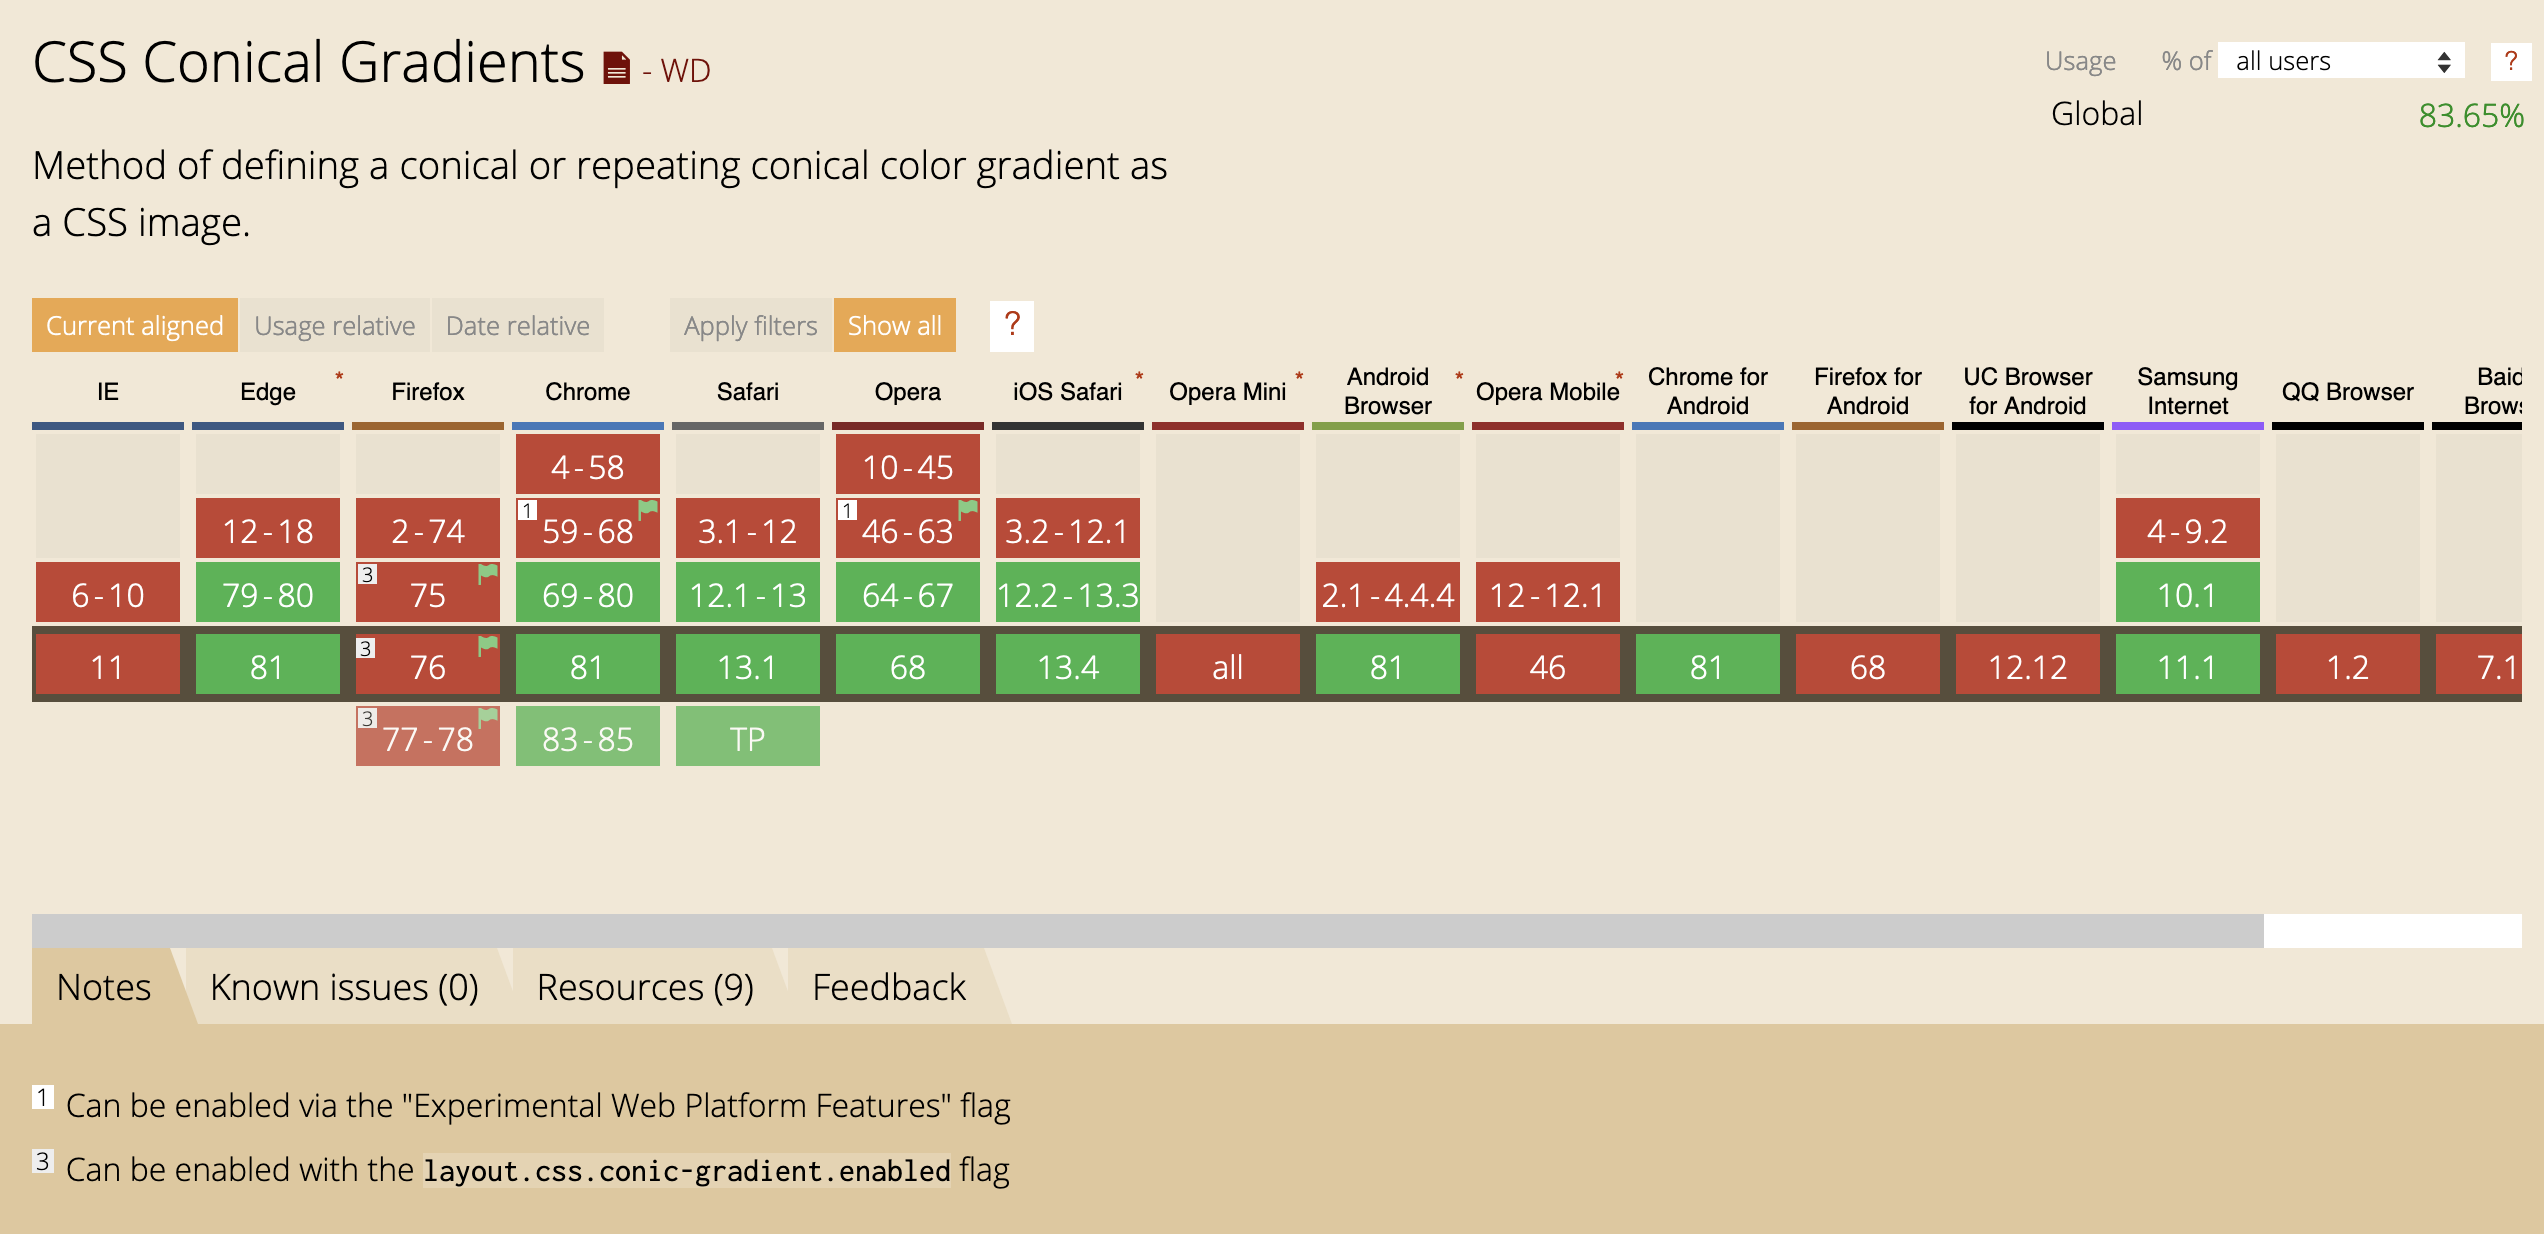
\includegraphics[width=\textwidth]{images/caniuse-after.png}
    \caption{Screenshot of Can I Use? as of May 6th}
\end{figure}

The interoperability of the implementation was evidenced by the contribution of new web platform tests, which also run in the Chromium and WebKit repositories. These tests also contribute to making other implementations more interoperable, as evidenced by an issue found in WebKit's implementation.

However, there are few things that were not achieved and could be potential future projects:

\begin{itemize}
    \item The implementation for the Cairo backend, only used for printers, is missing, due to the complexity of the backend. However, it is less important, since background images are disabled for printing unless a hidden preference is enabled, as mentioned in the Cairo section.
    \item The implementation for the Direct2D backend, used on the majority of Windows devices, has not been finished yet because of the lack of Windows development environment. With a Direct2D implementation done, Firefox could enable the conic gradient flag by default and catch up with the competition, as it was the only major browser to not implement the feature since January 2020.
    \item The current implementation is not fully-standard compliant yet as it does not allow mixing angles and percentages in \texttt{calc()} expressions. This is however less important for interoperability since no other web browser currently supports it.
    \item In retrospect, writing conic gradient tests for \texttt{border-image} would have been a good idea, since the web painting code uses a different code path for this case.
    \item An interesting fact was that conic gradients did not have an equivalent JavaScript API method for the HTML \texttt{<canvas>} element, since they are newer, despite the presence of equivalent methods for linear and radial gradients. A working implementation has been done but not merged. Contributing the API to the specification and adding a well-tested implementation to Firefox could be an interesting future potential project.
\end{itemize}

Regarding the Cairo and Direct2D backends, it is worth noting that those two implementations may not be necessary in the long term, since Mozilla is aiming to replace those backends with WebRender.


% =============================================================================

% Finally, after the main matter, the back matter is specified.  This is
% typically populated with just the bibliography.  LaTeX deals with these
% in one of two ways, namely
%
% - inline, which roughly means the author specifies entries using the 
%   \bibitem macro and typesets them manually, or
% - using BiBTeX, which means entries are contained in a separate file
%   (which is essentially a databased) then inported; this is the 
%   approach used below, with the databased being dissertation.bib.
%
% Either way, the each entry has a key (or identifier) which can be used
% in the main matter to cite it, e.g., \cite{X}, \cite[Chapter 2}{Y}.

\backmatter

\bibliography{dissertation}

% -----------------------------------------------------------------------------

% The dissertation concludes with a set of (optional) appendicies; these are 
% the same as chapters in a sense, but once signaled as being appendicies via
% the associated macro, LaTeX manages them appropriatly.

\appendix

\chapter{Conic Gradient syntax}
\label{appx:syntax}

\section{Conic gradient type}

The syntax for a conic gradient as defined in the specification \cite{conic-gradient-specification} is:

\begin{verbatim}
conic-gradient() = conic-gradient(
  [ from <angle> ]? [ at <position> ]?,
  <angular-color-stop-list>
)
\end{verbatim}

\begin{verbatim}
<angular-color-stop-list> =
  <angular-color-stop> , [ <angular-color-hint>? , <angular-color-stop> ]#
<angular-color-stop> = <color> && <color-stop-angle>?
<angular-color-hint> = <angle-percentage>
<color-stop-angle> = <angle-percentage>{1,2}

<color-stop> = <color-stop-length> | <color-stop-angle>
\end{verbatim}

\section{\texttt{<angle-percentage>} type}

In the CSS Values specification \cite{css-values-specification}, \texttt{<angle-percentage>} is defined as:

\begin{quote}
    Equivalent to \texttt{[ <angle> | <percentage> ]}, where the \texttt{<percentage>} will resolve to an \texttt{<angle>}.
\end{quote}

\noindent Also quoted from that last specification, \texttt{<angle>} is defined as a number followed by one of these units:
\begin{itemize}
\item \texttt{deg}

    Degrees. There are 360 degrees in a full circle. 

\item \texttt{grad}

    Gradians, also known as ``gons'' or ``grades''. There are 400 gradians in a full circle.

\item \texttt{rad}

    Radians. There are $2\pi$ radians in a full circle. 

\item \texttt{turn}

    Turns. There is 1 turn in a full circle.
\end{itemize}

\noindent while \texttt{<percentage>} is a number followed by a percentage sign.


\subsection{Examples}
\label{appx:syntax-examples}

The following examples are equivalent ways of expressing the same \texttt{<angle-percentage>} value:

\begin{itemize}
    \item \texttt{360deg}
    \item \texttt{1turn}
    \item \texttt{100\%}
    \item \texttt{400grad}
\end{itemize}

\noindent These can be combined within a \texttt{calc()} expression, like so:

\begin{itemize}
    \item \texttt{calc(360deg - 0.5turn)}
    \item \texttt{calc(100\% - 50\%)}
\end{itemize}

\noindent While this is not very useful in its current form, since \texttt{50\%} could be written directly, this is useful for use with CSS variables. The following example is adapted from Ana Tudor's metallic button demo \cite{metallic-button-demo}:

\begin{verbbox}[\small]
div {
    --step: 35deg;
    background: conic-gradient(
        gray,
        darkgray  var(--step), 
        lightgray calc(var(--step) * 2), 
        darkgray  calc(var(--step) * 3),
        lightgray calc(var(--step) * 4),
        gray      calc(var(--step) * 5),
        lightgray calc(var(--step) * 6),
        darkgray  calc(var(--step) * 7),
        gray      calc(var(--step) * 8),
        lightgray calc(var(--step) * 9),
        darkgray
    );
    width: 100px;
    height: 100px;
    border-radius: 100%;
}
\end{verbbox}
\begin{figure}[H]
    \vspace{20px}
    \hspace{0.05\textwidth}
    $\vcenter{\hbox{
\includegraphics[width=100px]{images/metallic-button.png}}}$
    \hspace{0.1\textwidth}
    $\vcenter{\hbox{\theverbbox}}$\qquad
    \vspace{20px}
    \caption{Simplified metallic button demo}
\end{figure}


The specification allows mixing angles and percentages in the same in the same expression \cite{mixing-percentages}, but no web browser currently supports it. The use-case is low, since percentages in this case are equivalent to angles anyway. For instance, \texttt{calc(100\% - 35deg)} could be written as \texttt{calc(1turn - 35deg)}, since the former is not supported.

\chapter{Placing color stops}
\label{appx:interpolation}
Quoted from the ``Placing color stops'' section of the specification \cite{interpolation-spec}:
\begin{quote}
Color stops are placed on a gradient line that curves around the gradient center in a circle, with both the \texttt{0\%} and \texttt{100\%} locations at \texttt{0deg}. Just like linear gradients, \texttt{0deg} points to the top of the page, and increasing angles correspond to clockwise movement around the circle.

Note: It may be more helpful to think of the gradient line as forming a spiral, where only the segment from \texttt{0deg} to \texttt{360deg} is rendered. This avoids any confusion about ``overlap'' when you have angles outside of the rendered region.

A color-stop can be placed at a location before \texttt{0\%} or after \texttt{100\%}; though these regions are never directly consulted for rendering, color stops placed there can affect the color of color-stops within the rendered region through interpolation or repetition (see repeating gradients). For example, \texttt{conic-gradient(red -50\%, yellow 150\%)} produces a conic gradient that starts with a reddish-orange color at \texttt{0deg} (specifically, \texttt{\#f50}), and transitions to an orangish-yellow color at \texttt{360deg} (specifically, \texttt{\#fa0}).

The color of the gradient at any point is determined by first finding the unique ray anchored at the center of the gradient that passes through the given point. The point’s color is then the color of the gradient line at the location where this ray intersects it.
\end{quote}

\noindent Here is how the example from the specification renders:

\begin{figure}[H]
    \centering
    
\includegraphics[width=150px]{images/special-color-stops.png}
    \caption{Rendering of \texttt{conic-gradient(red -50\%, yellow 150\%)}}
\end{figure}

\chapter{List of commits}
\label{appx:list-of-commits}

For historical purposes, this section provides a list of merged commits related to this project. 
\hspace{2em}

\begin{tabular}{ | m{3.25em} | m{22em} | m{2.8em} | m{4em} | m{5em} | m{2.8em} | } 
\hline
Bug ID & Commit message & Author & Reviewers & Merged on & Version \\
\hline
1614160 & Add AngleOrPercentage to style system & ntim & emilio & 2020-02-09 & 74 \\
\hline
1614648 & Make GradientItem and ColorStop support angular color stops & ntim & emilio & 2020-02-13 & 75 \\
\hline
1614890 & Implement conic-gradient for WebRender graphics backend & ntim & nical, emilio, gw &  2020-02-13 & 75 \\
\hline
1615489 & Refactor GenericGradient for conic-gradient support & ntim & emilio & 2020-02-16 & 75 \\
\hline
1615876 & Minor gradient parsing cleanup & emilio & ntim & 2020-02-16 & 75 \\
\hline
1615614 & Make brush\_conic\_gradient.glsl compile on GLES & ntim & gw & 2020-02-18 & 75 \\
\hline
1616106 & Add more tests and reference images for conic-gradient wrench test suite & ntim & nical & 2020-02-19 & 75 \\
\hline
1614202 & Implement parsing for CSS conic-gradient syntax & ntim & emilio & 2020-02-19 & 75 \\
\hline
1615862 & Handle conic-gradients in nsCSSGradientRenderer for WebRender & ntim & mstange, emilio & 2020-02-21 & 75 \\
\hline
1616587 & Implement conic-gradient for Skia graphics backend & ntim & lsalzman & 2020-02-21 & 75 \\
\hline
1617397 & Update WPT expectations for conic-gradient & ntim & jgraham & 2020-02-23 & 75 \\
\hline
1619006 & Fix max value in ReadElementConstrained call in RecordedEvent::ReadPatternData & ntim & nical & 2020-03-02 & 75 \\
\hline
1616255 & Handle normalized conic-gradient color stop positions in WebRender & ntim & gw & 2020-03-05 & 75 \\
\hline
1620328 & Set conic-gradient angle range on Skia & ntim & lsalzman & 2020-03-09 & 75 \\
\hline
1616986 & Add WPT reftests for conic-gradient and stop normalization & ntim & emilio & 2020-03-09 & 76 \\
\hline
1620951 & Fix definition of conic-gradient stopDelta in nsCSSGradientRenderer::Paint & ntim & emilio & 2020-03-09 & 76 \\
\hline
1621794 & Add DevTools support for conic-gradient() and repeating-conic-gradient() & ntim & gl & 2020-03-12 & 76 \\
\hline
1618997 & Improve serialization of conic and radial gradients & ntim & emilio & 2020-03-28 & 76 \\
\hline
1635818 & Fix some conic gradient WPT accidentally passing when conic gradients are unsupported & ntim & emilio & 2020-05-06 & 78 \\
\hline
\end{tabular}

\hspace{2em}

\begin{itemize}
    \item The bug IDs can be consulted on Bugzilla \cite{bugzilla}, which contains all the information related to the commit.
    \item The author and reviewers columns both include the usernames for succinctness.
    \item The ``Merged on'' date is the date the commit reached the mozilla-central repository.
    \item The ``Version'' column mentions in which Firefox version the commit is available.
\end{itemize}



\chapter{Support for mixing angle and percentages in \texttt{calc()} expressions}
\label{appx:unsupported-angle-percentage}

To test whether other browser engines (Blink and WebKit) support mixing angles and percentages in \texttt{calc()} expressions, it is possible to visit the following URL and check the rendering:

\begin{lstlisting}
data:text/html,<div style="background-image: conic-gradient(red calc(10deg + 25%), gold); width: 100px;height:100px"/>
\end{lstlisting}

\section{Blink}
Blink was checked by using Google Chrome Canary version 84 (latest experimental version).

\begin{figure}[H]
    \centering
    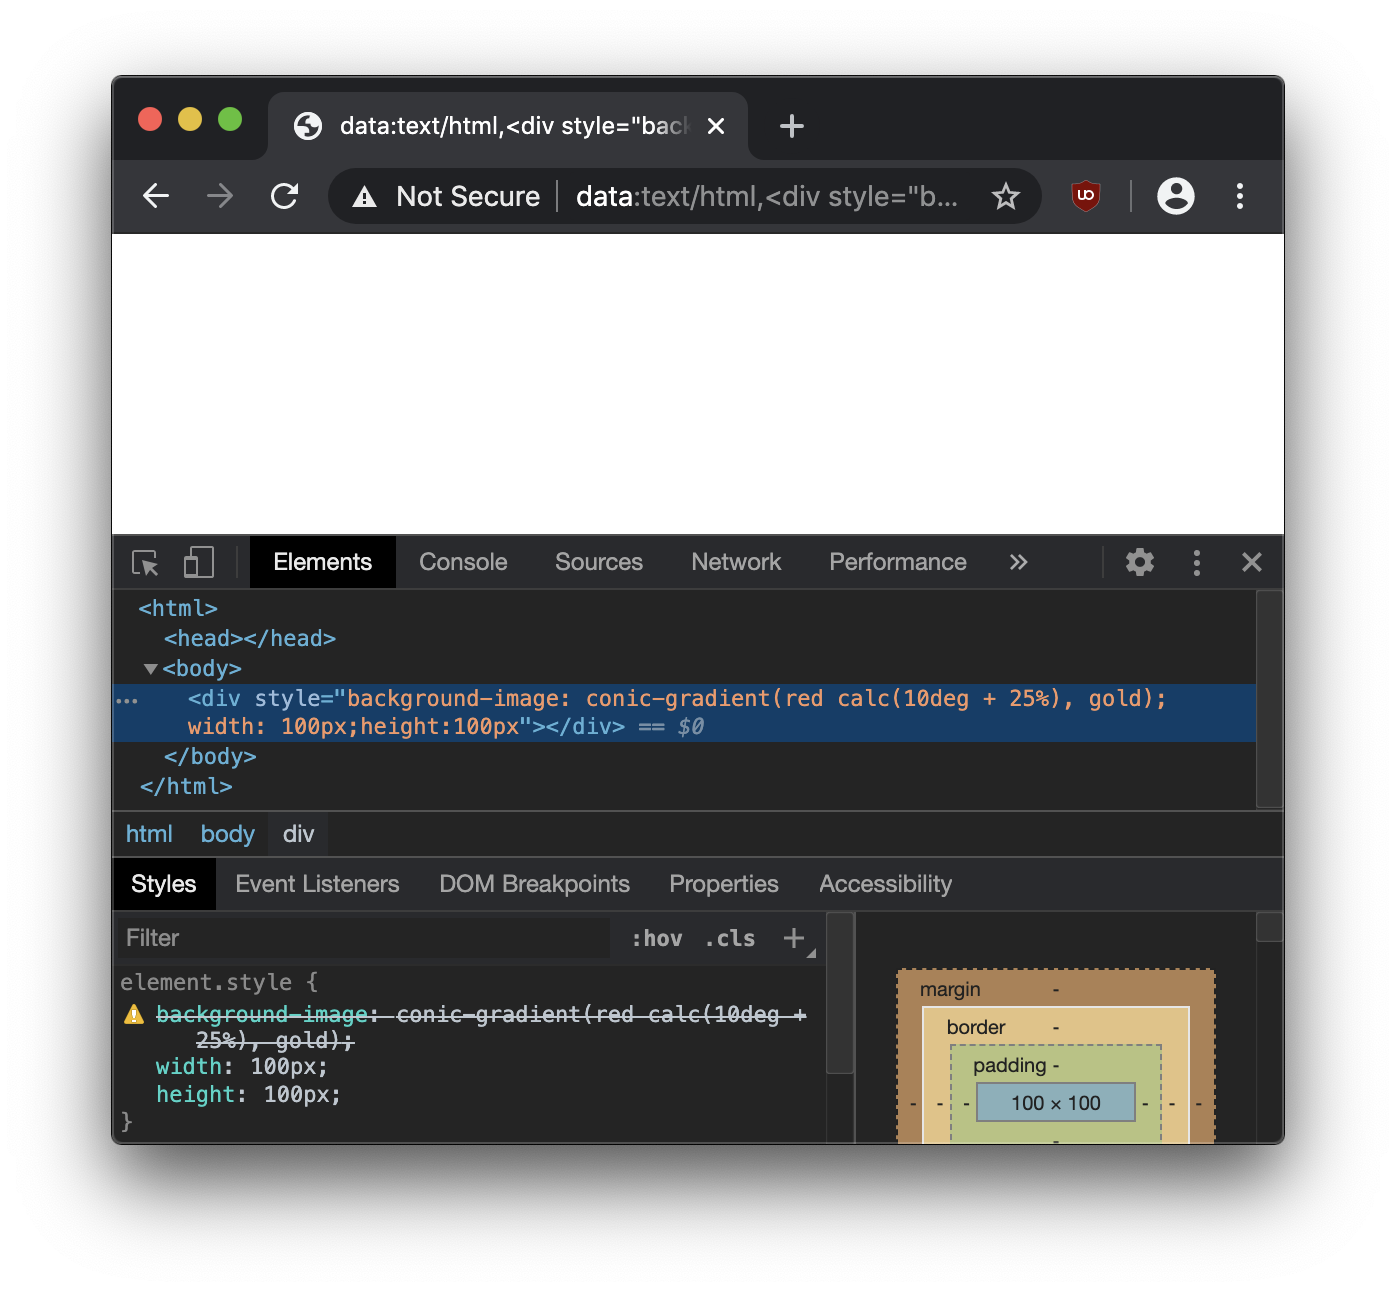
\includegraphics[width=0.75\textwidth]{images/testing-angle-percentage-blink.png}
    \caption{Testcase on Chromium}
\end{figure}

The value is not recognised as valid by the developer tools and Chrome renders a blank page, meaning it is not supported.

\section{WebKit}

Safari 13.1 (latest stable version) was checked, for the WebKit rendering engine.

\begin{figure}[H]
    \centering
    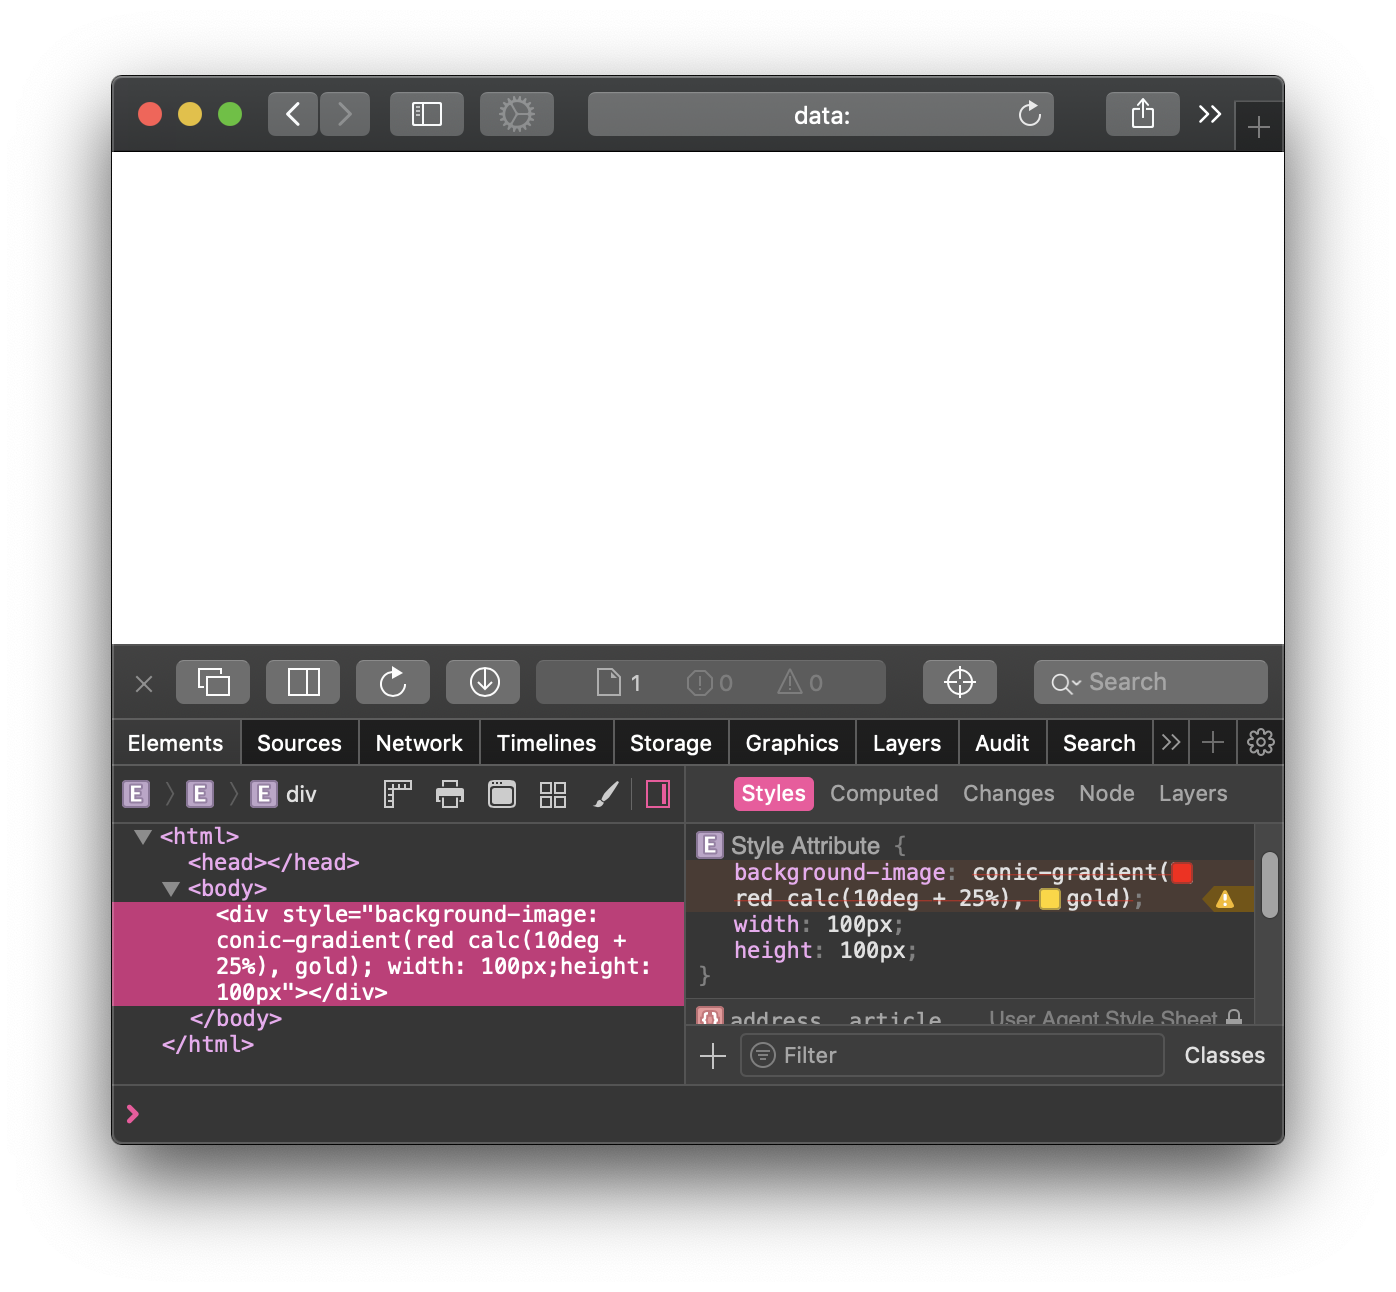
\includegraphics[width=\textwidth]{images/testing-angle-percentage-webkit.png}
    \caption{Testcase on Safari}
\end{figure}

The results are similar to Chrome: the value is not recognised as valid and the page is rendered blank.

\chapter{AngleOrPercentage code}
\section{Specified value implementation}
\label{appx:specified-angle-or-percentage}
\begin{minted}{rust}
/// <angle> | <percentage>
/// https://drafts.csswg.org/css-values/#typedef-angle-percentage
#[allow(missing_docs)]
#[derive(Clone, Copy, Debug, MallocSizeOf, PartialEq, SpecifiedValueInfo, ToCss, ToShmem)]
pub enum AngleOrPercentage {
    Percentage(Percentage),
    Angle(Angle),
}

impl AngleOrPercentage {
    fn parse_internal<'i, 't>(
        context: &ParserContext,
        input: &mut Parser<'i, 't>,
        allow_unitless_zero: AllowUnitlessZeroAngle,
    ) -> Result<Self, ParseError<'i>> {
        if let Ok(per) = input.try(|i| Percentage::parse(context, i)) {
            return Ok(AngleOrPercentage::Percentage(per));
        }

        Angle::parse_internal(context, input, allow_unitless_zero).map(AngleOrPercentage::Angle)
    }

    /// Allow unitless angles, used for conic-gradients as specified by the spec.
    /// https://drafts.csswg.org/css-images-4/#valdef-conic-gradient-angle
    pub fn parse_with_unitless<'i, 't>(
        context: &ParserContext,
        input: &mut Parser<'i, 't>,
    ) -> Result<Self, ParseError<'i>> {
        AngleOrPercentage::parse_internal(context, input, AllowUnitlessZeroAngle::Yes)
    }
}

impl Parse for AngleOrPercentage {
    fn parse<'i, 't>(
        context: &ParserContext,
        input: &mut Parser<'i, 't>,
    ) -> Result<Self, ParseError<'i>> {
        AngleOrPercentage::parse_internal(context, input, AllowUnitlessZeroAngle::No)
    }
}
\end{minted}

\chapter{Refactoring gradient code}
\label{appx:refactoring-gradient-code}
The full definition of the structures before and after the refactor of the gradient code is available in this appendix. The full diff for the refactor can be found at \cite{diff-refactor-style}. 

\section{Before}
\begin{minted}{rust}
/// A CSS gradient.
/// <https://drafts.csswg.org/css-images/#gradients>
#[derive(Clone, Debug, MallocSizeOf, PartialEq, ToComputedValue, ToResolvedValue, ToShmem)]
#[repr(C)]
pub struct GenericGradient<
    LineDirection,
    LengthPercentage,
    NonNegativeLength,
    NonNegativeLengthPercentage,
    Position,
    Color,
> {
    /// Gradients can be linear or radial.
    pub kind: GenericGradientKind<
        LineDirection,
        NonNegativeLength,
        NonNegativeLengthPercentage,
        Position,
    >,
    /// The color stops and interpolation hints.
    pub items: crate::OwnedSlice<GenericGradientItem<Color, LengthPercentage>>,
    /// True if this is a repeating gradient.
    pub repeating: bool,
    /// Compatibility mode.
    pub compat_mode: GradientCompatMode,
}
pub use self::GenericGradient as Gradient;

/// A gradient kind.
#[derive(Clone, Copy, Debug, MallocSizeOf, PartialEq, ToComputedValue, ToResolvedValue, ToShmem)]
#[repr(C, u8)]
pub enum GenericGradientKind<
    LineDirection,
    NonNegativeLength,
    NonNegativeLengthPercentage,
    Position,
> {
    /// A linear gradient.
    Linear(LineDirection),
    /// A radial gradient.
    Radial(
        GenericEndingShape<NonNegativeLength, NonNegativeLengthPercentage>,
        Position,
    ),
}
pub use self::GenericGradientKind as GradientKind;
\end{minted}

\section{After}
\begin{minted}{rust}
/// A CSS gradient.
/// <https://drafts.csswg.org/css-images/#gradients>
#[derive(Clone, Debug, MallocSizeOf, PartialEq, ToComputedValue, ToResolvedValue, ToShmem)]
#[repr(C)]
pub enum GenericGradient<
    LineDirection,
    LengthPercentage,
    NonNegativeLength,
    NonNegativeLengthPercentage,
    Position,
    Angle,
    AngleOrPercentage,
    Color,
> {
    /// A linear gradient.
    Linear {
        /// Line direction
        direction: LineDirection,
        /// The color stops and interpolation hints.
        items: crate::OwnedSlice<GenericGradientItem<Color, LengthPercentage>>,
        /// True if this is a repeating gradient.
        repeating: bool,
        /// Compatibility mode.
        compat_mode: GradientCompatMode,
    },
    /// A radial gradient.
    Radial {
        /// Shape of gradient
        shape: GenericEndingShape<NonNegativeLength, NonNegativeLengthPercentage>,
        /// Center of gradient
        position: Position,
        /// The color stops and interpolation hints.
        items: crate::OwnedSlice<GenericGradientItem<Color, LengthPercentage>>,
        /// True if this is a repeating gradient.
        repeating: bool,
        /// Compatibility mode.
        compat_mode: GradientCompatMode,
    },
}

pub use self::GenericGradient as Gradient;
\end{minted}


\chapter{nsCSSRenderingGradients changes}
\label{appx:nsCSSRenderingGradients-changes}
This is the combined diff of \texttt{nsCSSRenderingGradients.cpp} changes, over conic-gradient multiple commits (listed in chronological order):

\begin{enumerate}
    \item Tim Nguyen - Bug 1615862 - Handle conic-gradients in nsCSSGradientRenderer for WebRender. r=emilio,mstange (\texttt{https://phabricator.services.mozilla.com/D65994})
    \item Tim Nguyen - Bug 1616587 - Implement conic-gradient for Skia graphics backend. r=lsalzman (\texttt{https://phabricator.services.mozilla.com/D63415})
    \item Tim Nguyen - Bug 1620328 - Set conic-gradient angle range on Skia. r=lsalzman \newline (\texttt{https://phabricator.services.mozilla.com/D65910})
\end{enumerate}

\begin{minted}{diff}
@@ -225,6 +225,17 @@
   return MakeTuple(start, end, radiusX, radiusY);
 }

+// Compute the center and the start angle of the conic gradient.
+static Tuple<CSSPoint, float> ComputeConicGradientProperties(
+    const StyleGradient& aGradient, const CSSSize& aBoxSize) {
+  const auto& conic = aGradient.AsConic();
+  const Position& position = conic.position;
+  float angle = static_cast<float>(conic.angle.ToRadians());
+  CSSPoint center = ResolvePosition(position, aBoxSize);
+
+  return MakeTuple(center, angle);
+}
+
 static float Interpolate(float aF1, float aF2, float aFrac) {
   return aF1 + aFrac * (aF2 - aF1);
 }
@@ -459,7 +470,8 @@

 static ColorStop InterpolateColorStop(const ColorStop& aFirst,
                                       const ColorStop& aSecond,
-                                      double aPosition, const Color& aDefault) {
+                                      double aPosition,
+                                      const Color& aDefault) {
   MOZ_ASSERT(aFirst.mPosition <= aPosition);
   MOZ_ASSERT(aPosition <= aSecond.mPosition);

@@ -563,22 +575,40 @@
   return Some(pos.ResolveToCSSPixels(aLineLength) / aLineLength);
 }

-static nsTArray<ColorStop> ComputeColorStops(ComputedStyle* aComputedStyle,
-                                             const StyleGradient& aGradient,
-                                             CSSCoord aLineLength) {
-  auto items = aGradient.IsLinear() ? aGradient.AsLinear().items.AsSpan()
-                                    : aGradient.AsRadial().items.AsSpan();
+// aLineLength argument is unused for conic-gradients.
+static Maybe<double> GetSpecifiedGradientPosition(
+    const StyleGenericGradientItem<StyleColor, StyleAngleOrPercentage>& aItem,
+    CSSCoord aLineLength) {
+  if (aItem.IsSimpleColorStop()) {
+    return Nothing();
+  }
+
+  const StyleAngleOrPercentage& pos = aItem.IsComplexColorStop()
+                                          ? aItem.AsComplexColorStop().position
+                                          : aItem.AsInterpolationHint();

-  MOZ_ASSERT(items.Length() >= 2,
+  if (pos.IsPercentage()) {
+    return Some(pos.AsPercentage()._0);
+  }
+
+  return Some(pos.AsAngle().ToRadians() / (2 * M_PI));
+}
+
+template <typename T>
+static nsTArray<ColorStop> ComputeColorStopsForItems(
+    ComputedStyle* aComputedStyle,
+    Span<const StyleGenericGradientItem<StyleColor, T>> aItems,
+    CSSCoord aLineLength) {
+  MOZ_ASSERT(aItems.Length() >= 2,
              "The parser should reject gradients with less than two stops");

-  nsTArray<ColorStop> stops(items.Length());
+  nsTArray<ColorStop> stops(aItems.Length());

   // If there is a run of stops before stop i that did not have specified
   // positions, then this is the index of the first stop in that run.
   Maybe<size_t> firstUnsetPosition;
-  for (size_t i = 0; i < items.Length(); ++i) {
-    const auto& stop = items[i];
+  for (size_t i = 0; i < aItems.Length(); ++i) {
+    const auto& stop = aItems[i];
     double position;

     Maybe<double> specifiedPosition =
@@ -589,7 +619,7 @@
     } else if (i == 0) {
       // First stop defaults to position 0.0
       position = 0.0;
-    } else if (i == items.Length() - 1) {
+    } else if (i == aItems.Length() - 1) {
       // Last stop defaults to position 1.0
       position = 1.0;
     } else {
@@ -634,6 +664,21 @@
   return stops;
 }

+static nsTArray<ColorStop> ComputeColorStops(ComputedStyle* aComputedStyle,
+                                             const StyleGradient& aGradient,
+                                             CSSCoord aLineLength) {
+  if (aGradient.IsLinear()) {
+    return ComputeColorStopsForItems(
+        aComputedStyle, aGradient.AsLinear().items.AsSpan(), aLineLength);
+  }
+  if (aGradient.IsRadial()) {
+    return ComputeColorStopsForItems(
+        aComputedStyle, aGradient.AsRadial().items.AsSpan(), aLineLength);
+  }
+  return ComputeColorStopsForItems(
+      aComputedStyle, aGradient.AsConic().items.AsSpan(), aLineLength);
+}
+
 nsCSSGradientRenderer nsCSSGradientRenderer::Create(
     nsPresContext* aPresContext, ComputedStyle* aComputedStyle,
     const StyleGradient& aGradient, const nsSize& aIntrinsicSize) {
@@ -641,19 +686,26 @@

   // Compute "gradient line" start and end relative to the intrinsic size of
   // the gradient.
-  CSSPoint lineStart, lineEnd;
-  CSSCoord radiusX = 0, radiusY = 0;  // for radial gradients only
+  CSSPoint lineStart, lineEnd, center;  // center is for conic gradients only
+  CSSCoord radiusX = 0, radiusY = 0;    // for radial gradients only
+  float angle = 0.0;                    // for conic gradients only
   if (aGradient.IsLinear()) {
     Tie(lineStart, lineEnd) =
         ComputeLinearGradientLine(aPresContext, aGradient, srcSize);
-  } else {
+  } else if (aGradient.IsRadial()) {
     Tie(lineStart, lineEnd, radiusX, radiusY) =
         ComputeRadialGradientLine(aGradient, srcSize);
+  } else {
+    MOZ_ASSERT(aGradient.IsConic());
+    Tie(center, angle) = ComputeConicGradientProperties(aGradient, srcSize);
   }
   // Avoid sending Infs or Nans to downwind draw targets.
   if (!lineStart.IsFinite() || !lineEnd.IsFinite()) {
     lineStart = lineEnd = CSSPoint(0, 0);
   }
+  if (!center.IsFinite()) {
+    center = CSSPoint(0, 0);
+  }
   CSSCoord lineLength =
       NS_hypot(lineEnd.x - lineStart.x, lineEnd.y - lineStart.y);

@@ -677,6 +729,11 @@
   };
   renderer.mRadiusX = aPresContext->CSSPixelsToDevPixels(radiusX);
   renderer.mRadiusY = aPresContext->CSSPixelsToDevPixels(radiusY);
+  renderer.mCenter = {
+      aPresContext->CSSPixelsToDevPixels(center.x),
+      aPresContext->CSSPixelsToDevPixels(center.y),
+  };
+  renderer.mAngle = angle;
   return renderer;
 }

@@ -826,7 +883,8 @@
   double stopDelta = lastStop - firstStop;
   bool zeroRadius =
       mGradient->IsRadial() && (mRadiusX < 1e-6 || mRadiusY < 1e-6);
-  if (stopDelta < 1e-6 || lineLength < 1e-6 || zeroRadius) {
+  if (stopDelta < 1e-6 || (!mGradient->IsConic() && lineLength < 1e-6) ||
+      zeroRadius) {
     // Stops are all at the same place. Map all stops to 0.0.
     // For repeating radial gradients, or for any radial gradients with
     // a zero radius, we need to fill with the last stop color, so just set
@@ -869,8 +927,7 @@

     gradientPattern = new gfxPattern(gradientStart.x, gradientStart.y,
                                      gradientEnd.x, gradientEnd.y);
-  } else {
-    MOZ_ASSERT(mGradient->IsRadial());
+  } else if (mGradient->IsRadial()) {
     NS_ASSERTION(firstStop >= 0.0,
                  "Negative stops not allowed for radial gradients");

@@ -895,6 +952,9 @@
       matrix.PreScale(1.0, mRadiusX / mRadiusY);
       matrix.PreTranslate(-mLineStart);
     }
+  } else {
+    gradientPattern =
+        new gfxPattern(mCenter.x, mCenter.y, mAngle, stopOrigin, stopEnd);
   }
   // Use a pattern transform to take account of source and dest rects
   matrix.PreTranslate(gfxPoint(mPresContext->CSSPixelsToDevPixels(aSrc.x),
@@ -1120,7 +1180,8 @@
 void nsCSSGradientRenderer::BuildWebRenderParameters(
     float aOpacity, wr::ExtendMode& aMode, nsTArray<wr::GradientStop>& aStops,
     LayoutDevicePoint& aLineStart, LayoutDevicePoint& aLineEnd,
-    LayoutDeviceSize& aGradientRadius) {
+    LayoutDeviceSize& aGradientRadius, LayoutDevicePoint& aGradientCenter,
+    float& aGradientAngle) {
   aMode =
       mGradient->Repeating() ? wr::ExtendMode::Repeat : wr::ExtendMode::Clamp;

@@ -1136,6 +1197,8 @@
   aLineStart = LayoutDevicePoint(mLineStart.x, mLineStart.y);
   aLineEnd = LayoutDevicePoint(mLineEnd.x, mLineEnd.y);
   aGradientRadius = LayoutDeviceSize(mRadiusX, mRadiusY);
+  aGradientCenter = LayoutDevicePoint(mCenter.x, mCenter.y);
+  aGradientAngle = mAngle;
 }

 void nsCSSGradientRenderer::BuildWebRenderDisplayItems(
@@ -1151,8 +1214,10 @@
   LayoutDevicePoint lineStart;
   LayoutDevicePoint lineEnd;
   LayoutDeviceSize gradientRadius;
+  LayoutDevicePoint gradientCenter;
+  float gradientAngle;
   BuildWebRenderParameters(aOpacity, extendMode, stops, lineStart, lineEnd,
-                           gradientRadius);
+                           gradientRadius, gradientCenter, gradientAngle);

   nscoord appUnitsPerDevPixel = mPresContext->AppUnitsPerDevPixel();

@@ -1188,6 +1253,9 @@
   lineStart.x = (lineStart.x - srcTransform.x) * srcTransform.width;
   lineStart.y = (lineStart.y - srcTransform.y) * srcTransform.height;

+  gradientCenter.x = (gradientCenter.x - srcTransform.x) * srcTransform.width;
+  gradientCenter.y = (gradientCenter.y - srcTransform.y) * srcTransform.height;
+
   if (mGradient->IsLinear()) {
     lineEnd.x = (lineEnd.x - srcTransform.x) * srcTransform.width;
     lineEnd.y = (lineEnd.y - srcTransform.y) * srcTransform.height;
@@ -1199,8 +1267,7 @@
         mozilla::wr::ToLayoutPoint(lineEnd), stops, extendMode,
         mozilla::wr::ToLayoutSize(firstTileBounds.Size()),
         mozilla::wr::ToLayoutSize(tileSpacing));
-  } else {
-    MOZ_ASSERT(mGradient->IsRadial());
+  } else if (mGradient->IsRadial()) {
     gradientRadius.width *= srcTransform.width;
     gradientRadius.height *= srcTransform.height;

@@ -1211,7 +1278,15 @@
         mozilla::wr::ToLayoutSize(gradientRadius), stops, extendMode,
         mozilla::wr::ToLayoutSize(firstTileBounds.Size()),
         mozilla::wr::ToLayoutSize(tileSpacing));
+  } else {
+    MOZ_ASSERT(mGradient->IsConic());
+    aBuilder.PushConicGradient(
+        mozilla::wr::ToLayoutRect(gradientBounds),
+        mozilla::wr::ToLayoutRect(clipBounds), aIsBackfaceVisible,
+        mozilla::wr::ToLayoutPoint(gradientCenter), gradientAngle, stops,
+        extendMode, mozilla::wr::ToLayoutSize(firstTileBounds.Size()),
+        mozilla::wr::ToLayoutSize(tileSpacing));
   }
 }

 }  // namespace mozilla
\end{minted}
% =============================================================================

\end{document}
